\documentclass[11pt,a4paper,twoside]{book}\usepackage[]{graphicx}\usepackage[]{color}
%% maxwidth is the original width if it is less than linewidth
%% otherwise use linewidth (to make sure the graphics do not exceed the margin)
\makeatletter
\def\maxwidth{ %
  \ifdim\Gin@nat@width>\linewidth
    \linewidth
  \else
    \Gin@nat@width
  \fi
}
\makeatother

\definecolor{fgcolor}{rgb}{0.345, 0.345, 0.345}
\newcommand{\hlnum}[1]{\textcolor[rgb]{0.686,0.059,0.569}{#1}}%
\newcommand{\hlstr}[1]{\textcolor[rgb]{0.192,0.494,0.8}{#1}}%
\newcommand{\hlcom}[1]{\textcolor[rgb]{0.678,0.584,0.686}{\textit{#1}}}%
\newcommand{\hlopt}[1]{\textcolor[rgb]{0,0,0}{#1}}%
\newcommand{\hlstd}[1]{\textcolor[rgb]{0.345,0.345,0.345}{#1}}%
\newcommand{\hlkwa}[1]{\textcolor[rgb]{0.161,0.373,0.58}{\textbf{#1}}}%
\newcommand{\hlkwb}[1]{\textcolor[rgb]{0.69,0.353,0.396}{#1}}%
\newcommand{\hlkwc}[1]{\textcolor[rgb]{0.333,0.667,0.333}{#1}}%
\newcommand{\hlkwd}[1]{\textcolor[rgb]{0.737,0.353,0.396}{\textbf{#1}}}%
\let\hlipl\hlkwb

\usepackage{framed}
\makeatletter
\newenvironment{kframe}{%
 \def\at@end@of@kframe{}%
 \ifinner\ifhmode%
  \def\at@end@of@kframe{\end{minipage}}%
  \begin{minipage}{\columnwidth}%
 \fi\fi%
 \def\FrameCommand##1{\hskip\@totalleftmargin \hskip-\fboxsep
 \colorbox{shadecolor}{##1}\hskip-\fboxsep
     % There is no \\@totalrightmargin, so:
     \hskip-\linewidth \hskip-\@totalleftmargin \hskip\columnwidth}%
 \MakeFramed {\advance\hsize-\width
   \@totalleftmargin\z@ \linewidth\hsize
   \@setminipage}}%
 {\par\unskip\endMakeFramed%
 \at@end@of@kframe}
\makeatother

\definecolor{shadecolor}{rgb}{.97, .97, .97}
\definecolor{messagecolor}{rgb}{0, 0, 0}
\definecolor{warningcolor}{rgb}{1, 0, 1}
\definecolor{errorcolor}{rgb}{1, 0, 0}
\newenvironment{knitrout}{}{} % an empty environment to be redefined in TeX

\usepackage{alltt}
% We load package by package and set package relevant parameters.
% Topics are summarized later
%%%%%%%%%%%%%%%%%%%%%%%%%%%%%%%%%%%%%%%%%%%%%%%%%%%%%%%%%%%%%%%%%%%%%%%%
% helping packages
\usepackage{ifthen}
\usepackage{calc}

\usepackage[T1]{fontenc}       % provides fonts having  accented characters 
\usepackage[latin1]{inputenc}  % allows the user to input accented characters directly from the keyboard

%%%%%%%%%%%%%%%%%%%%%%%%%%%%%%%%%%%%%%%%%%%%%%%%%%%%%%%%%%%%%%%%%%%%%%%%

\renewcommand{\baselinestretch}{1.2}
\renewcommand{\textfraction}{0}%0.2     % placement of figures
\renewcommand{\topfraction}{1}%.3
\renewcommand{\bottomfraction}{1}%.3
\renewcommand{\floatpagefraction}{1}%.3
\setcounter{bottomnumber}{3}%1

\textwidth6.3in
\textheight9.7in
\topmargin-45pt
\oddsidemargin-.15in
\evensidemargin.15in
\headsep30pt
\headheight15pt
%\footskip20pt


%%%%%%%%%%%%%%%%%%%%%%%%%%%%%%%%%%%%%%%%%%%%%%%%%%%%%%%%%%%%%%%%%%%%%%%%

\usepackage[dvipsnames]{xcolor}
\definecolor{fgcolor}{rgb}{0.345, 0.345, 0.345}
\definecolor{shadecolor}{rgb}{.97, .97, .97}
\definecolor{messagecolor}{rgb}{0, 0, 0}
\definecolor{warningcolor}{rgb}{1, 0, 1}
\definecolor{errorcolor}{rgb}{1, 0, 0}
\definecolor{DarkBlue}{rgb}{0,0,0.5451}
\definecolor{DarkGreen}{rgb}{0,0.39216,0}
\definecolor{LightYellow}{rgb}{1,1,.8}
\definecolor{orange}{rgb}{.9,0.3445,0}



%%%%%%%%%%%%%%%%%%%%%%%%%%%%%%%%%%%%%%%%%%%%%%%%%%%%%%%%%%%%%%%%%%%%%%%%
\usepackage{afterpage}
\usepackage{natbib}
\usepackage{upquote}

\usepackage[english]{babel}

%%%%%%%%%%%%%%%%%%%%%%%%%%%%%%%%%%%%%%%%%%%%%%%%%%%%%%%%%%%%%%%%%%%%%%%%%%%%%%%
%% maxwidth is the original width if it is less than linewidth
%% otherwise use linewidth (to make sure the graphics do not exceed the margin)
\makeatletter
\def\maxwidth{ %
  \ifdim\Gin@nat@width>\linewidth
    \linewidth
  \else
    \Gin@nat@width
  \fi
}
\makeatother

%%%%%%%%%%%%%%%%%%%%%%%%%%%%%%%%%%%%%%%%%%%%%%%%%%%%%%%%%%%%%%%%%%%%%%%%%%%%%%%%%%%%%%%%%%%%%%%%%%%%%%%%%%%%
% from fancyvrb
\usepackage{fancyhdr}
\usepackage{fancyvrb}
\DefineVerbatimEnvironment{Rcode}{Verbatim}{xleftmargin=2em,fontshape=sl,formatcom=\color{DarkGreen}}
\fvset{listparameters={\setlength{\topsep}{0pt}}}

%%%%%%%%%%%%%%%%%%%%%%%%%%%%%%%%%%%%%%%%%%%%%%%%%%%%%%%%%%%%%%%%%%%%%%%%%%%%%%%%%%%%%%%%%%%%%%%%%%%%%%%%%%%%%
\usepackage{float}
\usepackage{graphicx}
\usepackage[margin=2em,labelfont=bf]{caption}


%%%%%%%%%%%%%%%%%%%%%%%%%%%%%%%%%%%%%%%%%%%%%%%%%%%%%%%%%%%%%%%%%%%%%%%%
\usepackage[pdftex,plainpages=false,pdfpagelabels,pagebackref=true,colorlinks=true,pdfpagemode=UseOutlines]{hyperref}


%%%%%%%%
\usepackage{tabularx}
%%%%%%%%

%%%%%%%%%%%%%%%%%%%%%%%%%%%%%%%%%%%%%%%%%%%%%%%%%%%%%%%%%%%%%%%%%%%%%%%%
% now math stuff and other details...
\usepackage{amsmath,amsthm,amssymb}

\newtheorem{pro}{Property}[chapter]
\theoremstyle{definition}
\newtheorem{des}{Definition}[chapter]
\newtheorem{bsp}{Example}[chapter]
\newtheorem{rem}{Remark}[chapter]

\newcommand*\widebar[1]{%
  \vbox{%
    \hrule height 0.5pt%     % Line above with certain width
    \kern0.5ex%             % Distance between line and content
    \hbox{%
      \kern-0.1em%           % Distance between content and left side of box, negative values for lines shorter than content
      \ifmmode#1\else\ensuremath{#1}\fi%  % The content, typeset in dependence of mode
      \kern-0.1em%      % Distance between content and left side of box, negative values for lines shorter than content
    }% end of hbox
  }% end of vbox
}
\def\ds{\displaystyle}

\newcommand{\rr}[1]{{\ttfamily\slshape\color{DarkGreen} #1}}

\makeatletter


% clever trick to circumvent potential redefines after loading packages:
% \providecommand{\something}{}  % if it does not exist, it creates it.
%      has same syntax as \newcommand
% \renewcommand{\something}{....}
% TUGboat 29(2)


\makeatletter
%umdefinierung exisitierender befehle
\let\oldH\H
\let\oldL\L
\let\oldO\H
\let\oldS\S
\let\olda\a
\let\oldb\b
\let\oldc\c
\let\oldd\d
\let\oldk\k
\let\oldv\v
\let\oldl\l
\let\oldt\t
\let\oldu\u
\let\oldIJ\IJ
\let\oldP\P
\let\P\relax
\let\oldnorm\|

%\DefineVerbatimEnvironment{CodeInput}{Verbatim}{fontshape=sl}
%\DefineVerbatimEnvironment{CodeOutput}{Verbatim}{}

% some classical environments, up-right, with chapter numbering.
\theoremstyle{definition}
\newtheorem{definition}{Definition}[chapter]
\newtheorem{example}{Example}[chapter]
\newtheorem{remark}{Remark}[chapter]
\newtheorem{theorem}{Theorem}[chapter]



\renewcommand{\|}{|\!|}         % closer norm
\newcommand{\T}{{}^{\top}}
\newcommand\code[1]{{\tt#1}}



\newcounter{algo}
\newenvironment{algorithm}{%
  \begin{list}{
      (\arabic{algo})
    }{
      \usecounter{algo}
    }%
}{
  \end{list}
}

% some text abbreviation
\newcommand{\GLS}{\text{GLS}}
\newcommand{\RR}{\text{RR}}
\newcommand{\OR}{\text{OR}}
\newcommand{\WLS}{\text{WLS}}
\newcommand{\MLE}{\text{MLE}}
\newcommand{\OLS}{\text{OLS}}
\newcommand{\MAE}{\text{MAE}}
\newcommand{\MAD}{\text{MAD}}
\newcommand{\RMSE}{\text{RMSE}}
\newcommand{\SVAR}{\text{svar}} %silvanos new commands
\newcommand{\EVAR}{\text{evar}}
\newcommand{\LMG}{\text{LMG}}
\newcommand{\Rtwo}{\text{R}^2}



\newcommand{\ii}{\text{\i}}

\newcommand{\Bin}{\cB\mathit{\!i\!n}}
\newcommand{\Beta}{\cB\mathit{\!e\!t\!a}}
\newcommand{\Pois}{\cP\mathit{\!o\!i\!s\!s\!o\!n}}
\newcommand{\Exp}{\cE\mathit{\!x\!p}}


\DeclareMathOperator*{\argmin}{argmin}
\DeclareMathOperator*{\argmax}{argmax}
\DeclareMathOperator{\diag}{diag}
\DeclareMathOperator{\diam}{diam}
\DeclareMathOperator{\card}{card}
\DeclareMathOperator{\cov}{Cov}                   
\DeclareMathOperator{\corr}{Corr}                 
\DeclareMathOperator{\var}{Var}                   
\DeclareMathOperator{\trace}{tr}                  
\DeclareMathOperator{\E}{E}                       
\DeclareMathOperator{\P}{P}                       
\DeclareMathOperator{\pred}{p}
\DeclareMathOperator{\vect}{vec}                  
\DeclareMathOperator{\vech}{vech}                 
\DeclareMathOperator{\rank}{rank}                 
\DeclareMathOperator{\e}{e}                       
%\DeclareMathOperator{\cv}{CV}                     
\DeclareMathOperator{\GCV}{GCV}                     
\DeclareMathOperator{\CV}{CV}                     
\DeclareMathOperator{\BLUP}{BLUP}                 
\DeclareMathOperator{\MSE}{MSE}                   
\DeclareMathOperator{\MS}{MS}                   
\DeclareMathOperator{\df}{df}                   
\DeclareMathOperator{\bias}{bias}                   
\DeclareMathOperator{\eig}{eig}                   
\DeclareMathOperator{\Prec}{Prec}
\DeclareMathOperator{\mode}{mode}
\renewcommand{\SS}{\text{SS}}
\renewcommand{\d}{\mathsf{\,d}}

\def\arctanh{\qopname\relax o{arctanh}}  % as in amsopn
\newcommand{\bigo}{\cO}
\newcommand{\lito}{\text{\scriptsize{$\cO$}}}
\newcommand{\cdfPhi}{\itPhi}
\newcommand{\ml}{_\text{ML}}

\newcommand*{\stack@relbin}[3][]{%
  \mathop{#3}\limits
  \toks@{#1}%
  \edef\reserved@a{\the\toks@}%
  \ifx\reserved@a\@empty\else_{#1}\fi
  \toks@{#2}%
  \edef\reserved@a{\the\toks@}%
  \ifx\reserved@a\@empty\else^{#2}\fi
  \egroup
}%
\renewcommand*{\stackrel}{\mathrel\bgroup\stack@relbin}
\newcommand*{\stackbin}{\mathbin\bgroup\stack@relbin}
\newcommand{\simiid}{\stackrel[]{\text{iid}}{\sim}}

% Kalligraphischer Schriftsatz
\newcommand{\cA}{{\cal{A}}}
\newcommand{\cB}{{\cal{B}}} 
\newcommand{\cC}{{\cal{C}}}
\newcommand{\cD}{{\cal{D}}} 
\newcommand{\cE}{{\cal{E}}}
\newcommand{\cF}{{\cal{F}}}
\newcommand{\cG}{{\cal{G}}}
\newcommand{\cH}{{\cal{H}}}
\newcommand{\cI}{{\cal{I}}}
\newcommand{\cJ}{{\cal{J}}}
\newcommand{\cK}{{\cal{K}}}
\newcommand{\cL}{{\cal{L}}}
\newcommand{\cM}{{\cal{M}}} 
\newcommand{\cN}{{\cal{N}}}
\newcommand{\cO}{{\cal{O}}} 
\newcommand{\cP}{{\cal{P}}}
\newcommand{\cQ}{{\cal{Q}}} 
\newcommand{\cR}{{\cal{R}}} 
\newcommand{\cS}{{\cal{S}}} 
\newcommand{\cT}{{\cal{T}}}
\newcommand{\cU}{{\cal{U}}}
\newcommand{\cV}{{\cal{V}}}
\newcommand{\cW}{{\cal{W}}}
\newcommand{\cX}{{\cal{X}}} 
\newcommand{\cY}{{\cal{Y}}}
\newcommand{\cZ}{{\cal{Z}}} 


\newcommand{\IA}{{\mathbb{A}}}
\newcommand{\IB}{{\mathbb{B}}}
\newcommand{\IC}{{\mathbb{C}}}
\newcommand{\ID}{{\mathbb{D}}}
\newcommand{\IE}{{\mathbb{E}}}
\newcommand{\IF}{{\mathbb{F}}}
\newcommand{\IG}{{\mathbb{G}}}
\newcommand{\IH}{{\mathbb{H}}}
\newcommand{\II}{{\mathbb{I}}}
%\newcommand{\IJ}{{\mathbb{J}}}
\newcommand{\IK}{{\mathbb{K}}}
\newcommand{\IL}{{\mathbb{L}}}
\newcommand{\IM}{{\mathbb{M}}}
\newcommand{\IN}{{\mathbb{N}}}
\newcommand{\IO}{{\mathbb{O}}}
\newcommand{\IP}{{\mathbb{P}}}
\newcommand{\IQ}{{\mathbb{Q}}}
\newcommand{\IR}{{\mathbb{R}}}
\newcommand{\IS}{{\mathbb{S}}}
\newcommand{\IT}{{\mathbb{T}}}
\newcommand{\IU}{{\mathbb{U}}}
\newcommand{\IV}{{\mathbb{V}}}
\newcommand{\IW}{{\mathbb{W}}}
\newcommand{\IX}{{\mathbb{X}}}
\newcommand{\IY}{{\mathbb{Y}}}
\newcommand{\IZ}{{\mathbb{Z}}}


% fette griechische kleinbuchstaben
\newcommand{\balpha}{{\boldsymbol{\alpha}}}
\newcommand{\bbeta}{{\boldsymbol{\beta}}}
\newcommand{\bgamma}{{\boldsymbol{\gamma}}}
\newcommand{\bdelta}{{\boldsymbol{\delta}}}
\newcommand{\blambda}{{\boldsymbol{\lambda}}}
\newcommand{\bepsilon}{{\boldsymbol{\epsilon}}}
\newcommand{\bvarepsilon}{{\boldsymbol{\varepsilon}}}
\newcommand{\bzeta}{{\boldsymbol{\zeta}}}
\newcommand{\bfeta}{{\boldsymbol{\eta}}}  %  <----- exception !
\newcommand{\btheta}{{\boldsymbol{\theta}}{}}
\newcommand{\bvartheta}{{\boldsymbol{\vartheta}}}
\newcommand{\biota}{{\boldsymbol{\iota}}}
\newcommand{\bkappa}{{\boldsymbol{\kappa}}}
\newcommand{\bmu}{{\boldsymbol{\mu}}}
\newcommand{\bnu}{{\boldsymbol{\nu}}}
\newcommand{\bxi}{{\boldsymbol{\xi}}}
\newcommand{\bpi}{{\boldsymbol{\pi}}}
\newcommand{\bvarpi}{{\boldsymbol{\varpi}}}
\newcommand{\brho}{{\boldsymbol{\rho}}}
\newcommand{\bvarrhoi}{{\boldsymbol{\varrho}}}
\newcommand{\bsigma}{{\boldsymbol{\sigma}}}
\newcommand{\bvarsigma}{{\boldsymbol{\varsigma}}}
\newcommand{\btau}{{\boldsymbol{\tau}}}
\newcommand{\bvartau}{{\boldsymbol{\vartau}}}
\newcommand{\bupsilon}{{\boldsymbol{\upsilon}}}
\newcommand{\bphi}{{\boldsymbol{\phi}}}
\newcommand{\bvarphi}{{\boldsymbol{\varphi}}}
\newcommand{\bchi}{{\boldsymbol{\chi}}}
\newcommand{\bpsi}{{\boldsymbol{\psi}}}
\newcommand{\bomega}{{\boldsymbol{\omega}}}


% fette griechische grossbuchstaben
\newcommand{\bGamma}{{\boldsymbol{\Gamma}}}
\newcommand{\bDelta}{{\boldsymbol{\Delta}}}
\newcommand{\bTheta}{{\boldsymbol{\Theta}}}
\newcommand{\bLambda}{{\boldsymbol{\Lambda}}{}}
\newcommand{\bXi}{{\boldsymbol{\Xi}}}
\newcommand{\bPi}{{\boldsymbol{\Pi}}}
\newcommand{\bSigma}{{\boldsymbol{\Sigma}}{}}
\newcommand{\bUpsilon}{{\boldsymbol{\Upsilon}}{}}
\newcommand{\bPhi}{{\boldsymbol{\Phi}}}
\newcommand{\bPsi}{{\boldsymbol{\Psi}}}
\newcommand{\bOmega}{{\boldsymbol{\Omega}}}

% italics griechische grossbuchstaben
\newcommand{\itGamma}{{\mathit{\Gamma}}}
\newcommand{\itDelta}{{\mathit{\Delta}}}
\newcommand{\itTheta}{{\mathit{\Theta}}}
\newcommand{\itLambda}{{\mathit{\Lambda}}}
\newcommand{\itXi}{{\mathit{\Xi}}}
\newcommand{\itPi}{{\mathit{\Pi}}}
\newcommand{\itSigma}{{\mathit{\Sigma}}}
\newcommand{\itUpsilon}{{\mathit{\Upsilon}}}
\newcommand{\itPhi}{{\mathit{\Phi}}}
\newcommand{\itPsi}{{\mathit{\Psi}}}
\newcommand{\itOmega}{{\mathit{\Omega}}}



\newcommand{\A}{{\mathbf{A}}}
\newcommand{\B}{{\mathbf{B}}}
\newcommand{\C}{{\mathbf{C}}}
\newcommand{\D}{{\mathbf{D}}}
\newcommand{\bfE}{{\mathbf{E}}}    % \E: expectation
\newcommand{\F}{{\mathbf{F}}}
\newcommand{\G}{{\mathbf{G}}}
\renewcommand{\H}{{\mathbf{H}}}
\newcommand{\I}{{\mathbf{I}}}
\newcommand{\J}{{\mathbf{J}}}
\newcommand{\K}{{\mathbf{K}}}
\renewcommand{\L}{{\mathbf{L}}}
\newcommand{\bfM}{{\mathbf{M}}}
\newcommand{\N}{{\mathbf{N}}}
\renewcommand{\O}{{\mathbf{O}}}
\newcommand{\bfP}{{\mathbf{P}}}  % \P : probability
\newcommand{\Q}{{\mathbf{Q}}}
\newcommand{\bfR}{{\mathbf{R}}}
\renewcommand{\S}{{\mathbf{S}}}
\newcommand{\bfT}{{\mathbf{T}}} % \T transpose
\newcommand{\U}{{\mathbf{U}}}
\newcommand{\V}{{\mathbf{V}}}
\newcommand{\W}{{\mathbf{W}}}
\newcommand{\X}{{\mathbf{X}}}
\newcommand{\Y}{{\mathbf{Y}}}
\newcommand{\Z}{{\mathbf{Z}}}


\newcommand{\0}{{\mathbf{0}}}
\newcommand{\1}{{\mathbf{1}}}
\newcommand{\2}{{\mathbf{2}}}
\newcommand{\3}{{\mathbf{3}}}
\newcommand{\4}{{\mathbf{4}}}
\newcommand{\5}{{\mathbf{5}}}
\newcommand{\6}{{\mathbf{6}}}
\newcommand{\7}{{\mathbf{7}}}
\newcommand{\8}{{\mathbf{8}}}
\newcommand{\9}{{\mathbf{9}}}

\renewcommand{\a}{{\textbf{\textit{a}}}}
\renewcommand{\b}{{\textbf{\textit{b}}}}
\renewcommand{\c}{{\textbf{\textit{c}}}}
\newcommand{\bfd}{{\textbf{\textit{d}}}}  % \d  'dx'
\newcommand{\bfe}{{\textbf{\textit{e}}}}  % \e  l'exponentiel
\newcommand{\f}{{\textbf{\textit{f}}}}
\newcommand{\g}{{\textbf{\textit{g}}}}
\newcommand{\h}{{\textbf{\textit{h}}}}
\newcommand{\bfi}{{\textbf{\textit{i}}}}%\i  complex i, sans 'dot'
\newcommand{\bfj}{{\textbf{\textit{j}}}}
\renewcommand{\l}{{\textbf{\textit{l}}}}
\renewcommand{\k}{{\textbf{\textit{k}}}}
\newcommand{\m}{{\textbf{\textit{m}}}}
\newcommand{\bfn}{{\textbf{\textit{n}}}}
\newcommand{\bfo}{{\textbf{\textit{o}}}}
\newcommand{\p}{{\textbf{\textit{p}}}}
\newcommand{\q}{{\textbf{\textit{q}}}}
\renewcommand{\r}{{\textbf{\textit{r}}}}
\newcommand{\s}{{\textbf{\textit{s}}}}
\renewcommand{\t}{{\textbf{\textit{t}}}}
\newcommand{\bfu}{{\textbf{\textit{u}}}} %\u used in references
\renewcommand{\v}{{\textbf{\textit{v}}}}
\newcommand{\w}{{\textbf{\textit{w}}}}
\newcommand{\x}{{\textbf{\textit{x}}}}
\newcommand{\y}{{\textbf{\textit{y}}}}
\newcommand{\z}{{\textbf{\textit{z}}}}




\ifcsname hlkwd\endcsname%    ... command '#1' exists ...%
\else%  ... command '#1' does not exist ...%

\def\maxwidth{ %
  \ifdim\Gin@nat@width>\linewidth
    \linewidth
  \else
    \Gin@nat@width
  \fi
}

\definecolor{fgcolor}{rgb}{0.345, 0.345, 0.345}
\newcommand{\hlnum}[1]{\textcolor[rgb]{0.686,0.059,0.569}{#1}}%
\newcommand{\hlstr}[1]{\textcolor[rgb]{0.192,0.494,0.8}{#1}}%
\newcommand{\hlcom}[1]{\textcolor[rgb]{0.678,0.584,0.686}{\textit{#1}}}%
\newcommand{\hlopt}[1]{\textcolor[rgb]{0,0,0}{#1}}%
\newcommand{\hlstd}[1]{\textcolor[rgb]{0.345,0.345,0.345}{#1}}%
\newcommand{\hlkwa}[1]{\textcolor[rgb]{0.161,0.373,0.58}{\textbf{#1}}}%
\newcommand{\hlkwb}[1]{\textcolor[rgb]{0.69,0.353,0.396}{#1}}%
\newcommand{\hlkwc}[1]{\textcolor[rgb]{0.333,0.667,0.333}{#1}}%
\newcommand{\hlkwd}[1]{\textcolor[rgb]{0.737,0.353,0.396}{\textbf{#1}}}%

\usepackage{framed}
\newenvironment{kframe}{%
 \def\at@end@of@kframe{}%
 \ifinner\ifhmode%
  \def\at@end@of@kframe{\end{minipage}}%
  \begin{minipage}{\columnwidth}%
 \fi\fi%
 \def\FrameCommand##1{\hskip\@totalleftmargin \hskip-\fboxsep
 \colorbox{shadecolor}{##1}\hskip-\fboxsep
     % There is no \\@totalrightmargin, so:
     \hskip-\linewidth \hskip-\@totalleftmargin \hskip\columnwidth}%
 \MakeFramed {\advance\hsize-\width
   \@totalleftmargin\z@ \linewidth\hsize
   \@setminipage}}%
 {\par\unskip\endMakeFramed%
 \at@end@of@kframe}
\renewenvironment{kframe}{%
 \def\at@end@of@kframe{}%
 \ifinner\ifhmode%
  \def\at@end@of@kframe{\end{minipage}}%
  \begin{minipage}{\columnwidth}%
 \fi\fi%
 \def\FrameCommand##1{\hskip\@totalleftmargin \hskip-0\fboxsep
 \colorbox{shadecolor}{##1}\hskip-0\fboxsep
     % There is no \\@totalrightmargin, so:
     \hskip-\linewidth \hskip-\@totalleftmargin \hskip\columnwidth}%
 \MakeFramed {\advance\hsize-\width
   \@totalleftmargin\z@ \linewidth\hsize
   \@setminipage}}%
 {\par\unskip\endMakeFramed%
 \at@end@of@kframe}


\definecolor{shadecolor}{rgb}{.97, .97, .97}
\definecolor{messagecolor}{rgb}{0, 0, 0}
\definecolor{warningcolor}{rgb}{1, 0, 1}
\definecolor{errorcolor}{rgb}{1, 0, 0}
%\newenvironment{knitrout}{}{} % an empty environment to be redefined in TeX
\newenvironment{knitrout}{\setlength{\topsep}{0mm}\setlength{\fboxsep}{4mm}}{} 

\usepackage{alltt}
\IfFileExists{upquote.sty}{\usepackage{upquote}}{}

  \fi%

\makeatother
   % packages, layout and standard macros
\IfFileExists{upquote.sty}{\usepackage{upquote}}{}
\begin{document}
\renewcommand\familydefault{\sfdefault} 
\pagenumbering{Alph}


\thispagestyle{empty}
\renewcommand{\baselinestretch}{1.5}\normalfont
\begin{center}
\setlength{\parindent}{0cm}
\bf\Large% 
The variable importance metric LMG  \\
applied to Bayesian linear regression models
\normalfont



\hrulefill

\vspace*{4cm}

\large
Master Thesis in Biostatistics (STA495) % or choose the next one
% Master Thesis in Mathematics (MAT491) 
\vspace*{12mm}

by

\vspace*{12mm}

Silvano Sele\\
\small 09 734 492\\
\normalfont
\vspace*{4cm}

supervised by

\vspace*{1cm}

Dr. Stefanie Muff\\
Name of supervisor (with title and affiliation if external)

\vfill

Zurich, September, 2018
\end{center}
\renewcommand\familydefault{\rmdefault}%
\renewcommand{\baselinestretch}{1.0}\rm 
\setcounter{page}{0}
\newpage
\vspace*{12cm}~\thispagestyle{empty}\pagenumbering{Roman}
\newpage


\graphicspath{{./figure/}}
\DeclareGraphicsExtensions{.pdf,.png}
\setcounter{tocdepth}{1}

\thispagestyle{empty}
\begin{center}
\vspace*{6cm}{\bfseries\Huge
  $p$-values:\\[5mm] their use, abuse and proper use \\[5mm]
  illustrated with seven facets 
}
\vfill
\rm

\LARGE
M\"axli Musterli\\[12mm]

\normalsize
Version \today
\end{center}
\newpage
\thispagestyle{empty}~
\newpage
\pagenumbering{roman}

\thispagestyle{plain}\markboth{Contents}{Contents}
\tableofcontents
\setkeys{Gin}{width=.8\textwidth}

\chapter*{Preface}
\addtocontents{toc}{\protect \vspace*{13.mm}}
\addcontentsline{toc}{chapter}{\bfseries{Preface}}
\thispagestyle{plain}\markboth{Preface}{Preface}

Howdy!

\bigskip

\begin{flushright}
Max Muster\\
June 2018
\end{flushright}

\addtocontents{toc}{\protect \vspace*{10mm}}

\cleardoublepage
\pagenumbering{arabic}


%%%%%%%%%%%%%%%%%%%%%%%%%%%%%%%%%%%%%%%%%%%%%%%%%%%%%%%%%%%%%%%%%%%%%% 



% LaTeX file for Chapter 01







\chapter{Introduction}

The aim of this master thesis is to implement the variable importance measure LMG  (named after the authors Lindeman, Merenda, and Gold \citep{Gromping2007}) in linear models estimated with Bayesian methods. 

Regression models are popular in many applied research areas \citep{Nimon2013}. These models provide a tool to find an association between a response variable Y and a set of explanatory variables. The explanatory variables are also called predictors or covariates. Regression parameters provide us the information how much the response variable is expected to change when a predictor changes by one unit, given all other predictors in the model stay the same. The last subsentence is very important for the correct interpretation of the regression parameters. It shows also that the parameter value of a predictor is dependent on the other predictors in the model.

Because predictors are often correlated to some degree to each other, it is clear that it is not an easy task to find the most important predictors in a model. The first question then is: What do we  mean by the importance of a predictor? A question that is not easy answered and depending on the research question. \cite{Gromping2015} concludes that there may never  be a unique accepted definition of what variable importance is. Different metrics exist to quantify the importance of predictors. These metrics focus on different aspects and with correlated predictors they  lead to different conclusions.  A summary of the metrics can be found in  \cite{Gromping2015}.  

A distinction should be made between the importance of predictors in regression models that are used to predict future data and regression models who wish to find an association between predictors and the response variable. In the former case, the aim is only to reduce the error between the predicted values and the real observed values. It does not really matter how we get there. In the other case, we are interested in the strength of the relationship between the predictors and the response variable. A predictor may explain little of the response variable given two other correlated predictors are already included in a regression model. However, this from the regression output unimportant predictor may be the main cause of the other two predictor values.  It therefore may somehow be the most important predictor in this model \citep{Gromping2007}. 

The causal relationship between the variables is missing in the regression model. Regressing conditional on  other variables or using univariate regression models only provide us some parts of the bigger picture about the predictor in a model. Some authors recommend that the variable importance metric is based on both components.  Which variable importance metrics are the most useful ones is still an open debate. A convincing theoretical basis is still lacking for all of them.  \cite{Gromping2015} recommends to use the existing best practices, until a more profound solution is found. For variance (or generally goodness of fit) decomposition based importance, she recommends to use LMG enhanced with joint contributions or dominance analysis \citep{Gromping2007}.  


% LaTeX file for Chapter 02








\chapter{Methods} 

\section{LMG variable importance metric}

The focus of this master thesis is on the LMG variable importance metric. The LMG is a metric that is based on variance decomposition. The total $\Rtwo$ of a model is decomposed onto the predictors. Marginal and conditional information are incorporated \citep{Gromping2015} .  The following formulas are taken from \cite{Gromping2015}. The same mathematical notations are used. 

The following  notations for the explained variance (1) and sequentially added variance (2) simplify the notation of the LMG formula. 

   \begin{align} 
     \EVAR(S) = \var(Y) - \var( Y \mid X_{j}, j \in S),   \label{eq:1} 
   \end{align} 
   \begin{align} 
     \SVAR(M \mid S) = \EVAR(M \cup S) - \EVAR(S), \label{eq:2} 
    \end{align} , where $S$ and $M$ denote disjoint sets of predictors.
    
   The LMG formula is given below for the first predictor only. Because of exchangeable predictors, this is no loss of generality.  $\Rtwo(S)$ can be written as $\EVAR(S)/\var(Y).$ 

   \begin{align*} 
     \LMG(1) &= \frac{1}{p!} \sum_{\pi permutation}^{} \SVAR(\{1\} \mid S_{1}(\pi)),   \nonumber  \\
     &= \frac{1}{p!} \sum_{S \subseteq \{ 2, \dots, p \} }^{} n(S)! \, (p-n(S)-1)! \, \SVAR(\{1\} \mid S) \nonumber  \\
     &=  \cfrac{1}{p} \sum_{i=0}^{p-1} \left( \substack {\sum\limits_{ S \subseteq \{ 2, \dots, p \}}\\n(S)=1}^{} \ \SVAR(\{1\} \mid S)\right)\bigg/ \binom{p-1}{i}  \nonumber \\   
         &=  \cfrac{1}{p} \sum_{i=0}^{p-1} \frac{ \substack{\sum\limits_{ S \subseteq \{ 2, \dots, p \}}\\n(S)=1}^{} \ \SVAR(\{1\} \mid S)}{\binom{p-1}{i}}, \nonumber \\      
   \end{align*}
   where $S_{1}(\pi)$ is the set of predecessors of predictor 1.
   
   The different writings of the formula help to better understand what is calculated in the LMG metric. The $\Rtwo$ of the model including all predictors is decomposed. In the top formula the LMG value of predictor 1 is represented as an unweighted average over all orderings of the sequential added variance contribution of predictor 1. The middle formula shows that the calculation can be  done computationally more efficient. The orderings with the same set of predecessors $S$ are combined into one summand. Instead of $p!$ summands only $2^{p-1}$ summands need to be calculated. The bottom formula shows that the LMG metric can also be seen as the unweighted average over average explained variance improvements when adding predictor 1 to a model of size i without predictor 1 \citep{Gromping2015}. The LMG metric is implemented in the R package relaimpo \citep{Gromping2006}.
   
\cite{Chevan1991} propose that instead of only using the variances, an appropriate goodness-of-fit metric can as well be used in the LMG formula. They name their proposal hierarchical partitioning. The requirements are simply: an initial measure of fit when no predictor variable is present, a final measure of fit when N predictor variables are present, all intermediate models when various combinations of predictor variables are present. 
  The LMG component of each variable is named independent component (I). The sum of the independent components (I) results then in the overall goodness-of-fit metric. The difference between the goodness-of-fit when only the predictors itself is included in the model, compared to its independent component (I) is named the joint contribution (J). Hierarchical partitioning is implemented in the hier.part package \citep{Walsh2015}. The LMG values are calculated when  $\Rtwo$ is chosen as the goodness-of-fit measure.  The partitioning function of the hier.part package is used in this master thesis. The hierarchical partitioning function accepts as input a data frame with the $\Rtwo$ values of all submodels. Of note,  the hier.part package is only guaranteed to work for 9 predictors and does not work at all for more than 12 predictors.
  
\section{ Appropriate $\Rtwo$ definitions in the Bayesian framework}
The focus of this master thesis is on the linear model. For the linear model the $\Rtwo$ is the most widely used goodness-of-fit metric.  Different formulas for $\Rtwo$ exist \cite{Kvalseth1985}, all leading to the same value when and intercept is included and the model is fitted by maximum likelihood. 

Two popular definitions are:
   
      \begin{align} 
     R^2 &= 1 - \frac{\sum_{i=1}^{n}(y_{i} - \hat{y_{i}})^2}{\sum_{i=1}^{n}(y_{i}-\bar{y})^2}   \label{eq:rtwo1} \\
     R^2 &= \frac{\sum_{i=1}^{n}(\hat{y_{i}} - \bar{y})^2}{\sum_{i=1}^{n}(y_{i}-\bar{y})^2}, \qquad i = 1,\dots,n,   \label{eq:rtwo2} 
   \end{align} 
   
, where $\hat{y_{i}} = = \E ({y \mid X_{i}, \hat{\theta}})$.  $\hat{\theta}$ is the maximum likelihood estimate of the regression coefficients.


When other estimation methods than maximum likelihood are used \eqref{eq:rtwo1} can be negative and \eqref{eq:rtwo2}  can be bigger than 1. This is not uncommon in a Bayesian regression setting, when samples of the posterior parameter distribution are employed. A model that explaines more than 100\% of the variance does not make sense. A negative $\Rtwo$ is also difficult to interpret. A negative $\Rtwo$ may be interpreted as a fit that is worse than the mean of the data. This can make sense for predictive purposes, e.g. when new data from a test set is predicted by leave-one-out crossvalidation \citep{Alexander2015}.  For non predicting purposes a negative $\Rtwo$ does not make sense. The aim of the LMG formula is to gain some more information about the possible association between variables. A predictor can not explain less than zero variance in the population. To respect the non-negative share property of the LMG formula the $\Rtwo$ of submodels should not decrease when adding predictors. Both classical $\Rtwo$ definitions seem not to be well suited for the LMG metric in the Bayesian framework.

A more reasonable $\Rtwo$ definition for the LMG formula in the Bayesian framework can be found by noting that the variance of the linear model can also be written as 

      \begin{align} 
        \var(y) = \var(\X \bbeta) + \sigma^2 = \bbeta^\top \bSigma_{\X \X}  \bbeta + \sigma^2, \label{eq:vary} 
   \end{align}
where $\bbeta^\top = (\beta_{1} \dots \beta_{p})$ are the regression parameters without the intercept.
$\bSigma_{\X \X}$ is the covariance matrix of the regressors.

By using this variance definition \cite{Gelman2017} proposes to use 

      \begin{align} 
       \Rtwo_{Gelman} = \frac{\var(\sum_{i=1}^{n}\hat{y}^s_{i})}{\var(\sum_{i=1}^{n}\hat{y}^s_{i})+\var(\sum_{i=1}^{n}e^s_{i})}, \qquad i = 1,\dots,n, \label{rtwoGelman} 
   \end{align} 
   
, where $\hat{y}^s_{i}  = \E \left({y \mid X_{i}, \theta^s}\right) $ and the vector of errors $e^s_{i} = y_{i} - \hat{y}^s_{i}$ and $\theta^s, s = 1,\dotsc, S$ are draws from the posterior parameter distribution. The formula is then guaranteed to be between 0 and 1. The $\Rtwo$ can  be interpreted as a data-based estimate of the proportion of variance explained for new data under the assumption that the predictors are held fixed \citep{Gelman2017}.

In the Bayesian framework the $\sigma^2$ parameter is explicitly modeled in the standard linear regression setting. It is therefor possible to sample the $\sigma^2$ parameter from its posterior distribution instead of defining the error as in \eqref{rtwoGelman}, which would lead to the following definition:

    \begin{align} 
        \Rtwo &= \frac{\var(\sum_{i=1}^{n}\hat{y}^s_{i})}{\var(\sum_{i=1}^{n}\hat{y}^s_{i})+\sigma_{s}^2} \\ &= \frac{\bbeta_{s}^\top \bSigma_{\X \X}  \bbeta_{s}}{\bbeta_{s}^\top \bSigma_{\X \X}  \bbeta_{s}+\sigma_{s}^2}\label{rtwoused} 
   \end{align} 
 , where $\hat{y}^s_{i}  = E \left({y \mid X_{i}, \theta^s}\right) $,  and $\theta^s, s = 1,\dotsc, S$ are draws from the posterior parameter distribution.


The predictors in \eqref{rtwoGelman} and \eqref{rtwoused} could also be taken as random \citep{Gelman2017}. The predictors are then called stochastic predictors. Using the sample covariance estimate provides us then just an estimate of the true covariance structure. With stochastic predictors there is an additional uncertainty in the $\Rtwo$ formula that can have a large influence on the $\Rtwo$ and especially the LMG values.

In practice \eqref{rtwoused} and \eqref{rtwoGelman} should lead to  similar values in the standard linear model. In my opinion it is more reasonable to go the full Bayesian route and sample  $\sigma^2$. This provides us the opportunity to include prior information about $\sigma^2$ directly into to $\Rtwo$ calculations. The LMG calculations in the examples of this master thesis will therefore be based on \eqref{rtwoused}.  The benefit of \eqref{rtwoGelman} is that it also works for generalized linear models, where we often have no separate variance parameter.

 The denominator of $\Rtwo$ is no longer fixed in \eqref{rtwoGelman} and \eqref{rtwoused}. We can therefore no longer interpret an increase in $\Rtwo$ as an improved fit to a fixed target \citep{Gelman2017}. This seems to be problematic for the LMG formula in the Bayesian framework. However, in the linear model it is possible to calculate the $\Rtwo$ of all submodels from the parameters of the fullmodel and the covariance matrix of the predictors. We therefore compare all submodels of a posterior sample to the same fixed value. How it is possible to get the $\Rtwo$ of the submodels from the full model is shown in the next section.

\section{Conditional variance formula}


For two predictors \eqref{eq:vary} simplifies to

      \begin{align} 
        \var(y) = \beta_{1}^2 \var(X_{1}) + 2  \beta_{1}  \beta_{2} \cov(X_{1}, X_{2}) + \beta_{2}^2 \var(X_{2}) + \sigma^2, \label{varx1x2} 
   \end{align}
 
 When predictor $X_{1}$ is alone in the model the explained variance includes the variance of the predictor itself, the whole covariance term and in addition some of the contribution of the variance of $X_{2}$ in \eqref{varx1x2} . In mathematical notation that is
 
      \begin{align} 
        \SVAR({X_{1}} \mid \emptyset ) = \beta_{1}^2 \var(X_{1}) + 2  \beta_{1}  \beta_{2} \cov(X_{1}, X_{2}) + \beta_{2}^2 \var(X_{2}) \rho_{12}^2 \nonumber 
   \end{align}
   
The contribution of the second regressor is then simply the difference to the total explained variance \citep{Gromping2007}. 

In the general case with $p$ regressors, the conditional variance formula \eqref{eq:condvar} can be used to calculate the $\Rtwo$ of all submodels. The conditional variance formula can for example be used to specify the conditional distribution of a multivariate normal distribution $\Y$ .

The elements of the vector $\Y$ are reordered as
\begin{align*}
\mathbf{Y} = \begin{pmatrix}
\mathbf{Y}_{1} \\ 
\mathbf{Y}_{2} \end{pmatrix}, \mathbf{Y}_{1} \in \IR^q, \mathbf{Y}_{2} \in \IR^{p-q} .
\end{align*}

The joint distribution is a multivariate normal distribution with elements
\begin{align*}
\begin{pmatrix}
\mathbf{Y}_{1} \\ 
\mathbf{Y}_{2} \end{pmatrix} \sim \mathcal{N}
\Bigg(\begin{pmatrix}
\boldsymbol{\mu}_{1} \\ 
\boldsymbol{\mu}_{2} 
\end{pmatrix},
\begin{pmatrix}
\bSigma_{11} & \bSigma_{12} \\
\bSigma_{21} & \bSigma_{22} \\
\end{pmatrix}\Bigg),
\ \bSigma_{21} = \bSigma_{12}^{T},
\end{align*}
the conditional distribution is normally distributed again with mean 
\begin{align*}
\E (\mathbf{Y}_{1} | \mathbf{y}_{2} ) = \boldsymbol{\mu}_{1}\ +\ \bSigma_{12} \bSigma_{22}^{-1}(\mathbf{Y}_{2}\ -\ \boldsymbol{\mu}_{2})
\end{align*}
and the conditional variance is
\begin{align}
\var ( \mathbf{Y}_{1} | \mathbf{y}_{2} ) = \bSigma_{11}\ -\ \bSigma_{12} \bSigma_{22}^{-1}\bSigma_{21} \text{.} \label{eq:condvar} 
\end{align}

The aim is to calculate $\Rtwo$ of a submodel containining the predictors $\X_{q...p}$, and regression coefficients $\bbeta^\top = (\beta_{1}, \dotsc, \beta_{p})$ without the intercept. The regression coefficients are further separated in $\bbeta^\top_{1  ,\dotsc,  q-1} = (\beta_{1} ,\dotsc, \beta_{q-1})$ and $\bbeta^\top_{q ,\dotsc, p} = (\beta_{q} ,\dotsc, \beta_{p})$. 

As in the multivariate normal distribution example above, the covariance matrix of $p$ predictors is written as 

      \begin{align*} 
\cov(\X) =	\bSigma_{\X \X} = \begin{pmatrix}
\bSigma_{11} & \bSigma_{12} \\
\bSigma_{21} & \bSigma_{22}  \\
\end{pmatrix}^{p \times p}, 
   \end{align*}
   
         \begin{align*} 
   \text{where} \qquad \bSigma_{11} &= \cov(\X_{1,\dotsc, q-1}, \X_{1 ,\dotsc,q-1}), \\ \bSigma_{12} &= \cov(\X_{1,\dotsc, q-1}, \X_{q ,\dotsc, p}),\\ \bSigma_{22} &= \cov(\X_{q ,\dotsc, p}, \X_{q \dots p}) \text{.} \nonumber
      \end{align*}
      
 The conditional variance of the predictors $ \X_{1 ,\dotsc, q-1} $ given the predictors  $ \X_{q ,\dotsc, p} $ is then
 
          \begin{align*} 
 \cov(\X_{1,\dotsc, q-1} \mid \x_{q ,\dotsc, p}) = \bSigma_{11}\ -\ \bSigma_{12} \bSigma_{22}^{-1}\bSigma_{21} .
       \end{align*}
       
       The total explained variance of the full model $\X_{1 \dots p}$ omits simply the $\sigma^2$ parameter in \eqref{eq:vary} , which is

      \begin{align*} 
        \EVAR(\X_{1 ,\dotsc, p}) = \bbeta^\top \bSigma_{\X \X}  \bbeta. 
   \end{align*}

The explained variance of a submodel can be calculated by subtracting from the total explained variance the explained variance of the not-in-the-model-included-predictors that is not explained by in-the-model-included-predictors. The variance that is not explained by in-the-model-included-predictors is given by the variance of the not-in-the-model-included predictors conditional on the in-the-model-included-predictors. The explained variance of a submodel containing predictors $\X_{q ,\dotsc, p}$ can therefore be written as

       \begin{align} 
       \EVAR(\X_{q \dots p}) =  \EVAR(\X_{1  ,\dotsc, p}) - \bbeta^\top_{1 ,\dotsc, q-1} \cov(\X_{1,\dotsc, {q-1}} \mid \x_{q \dots p}) \bbeta_{1 ,\dotsc, {q-1}} . \label{eq:varsub} 
   \end{align}

To gain the the $\Rtwo$ value of the submodel we need to divide the explained variance by the total variance, which is
       \begin{align*} 
\EVAR(\X_{q ,\dotsc, p}) / \var(\Y),   
\end{align*}

where $\var(\Y)$ is definied as  $\bbeta^\top \bSigma_{\X \X}  \bbeta + \sigma^2$.



A posterior density distribution is obtained for the regression parameters in the Bayesian regression setting. The LMG formula requires calculation of the $\Rtwo$ values for all $2^p-1$ submodels. Samples from the joint posterior paramters of the full model are used to calculate the explained variance of the  submodels. For each sample the  conditional variance formula is used to obtain the $\Rtwo$ of the $2^p-1$ submodels. The property that all shares should be non-negative and the dependence of the parameter values from the submodels to each other is then respected for each sample. 

Instead of using the conditional mean formula to get the $\Rtwo$ of the submodels,  it would be possible to fit a separate Bayesian model for each submodel. An $\Rtwo$ distribution can easily be built for each submodel by using \eqref{rtwoGelman} or  \eqref{rtwoused}. However, the problem is how to calculate the LMG values out of these $\Rtwo$ distributions. If we just sample independently from the $\Rtwo$ distributions, the dependence of the paramter values of the submodels to each other is ignored. We would have many possibly true parameter values of a predictor in the same LMG comparison. It would then also be possible that the $\Rtwo$ decreases when adding predictors.  Another drawback is that it would be much more time consuming to fit a separate Bayesian model for each submodel. Using the conditional variance formula on the full model allows us to calculate LMG values in the Bayesian framework in a reasonable amount of time. Depending on the number of predictors and the number of posterior samples, the calculations still take some time in the Bayesian framework. For stochastic predictors the computation time is multiplied by the number of covariance samples.


\section{Bayesian Regression}
This Section provides a short introduction to Bayesian regression. It further shows that assuming stochastic or non-stochastic predictors results in the same posteriors for the regression parameters under some assumptions.  It is summarized from the book Bayesian Analysis for the Social Sciences \citep{Jackman2009}. 

In regression analysis we are interested in the dependence of $\y$ on $\X$. The conditional mean of a continuous response variable $\y = (y_{1}, \dots, y_{n})^\top$ is related to a $n \times k$ predictor matrix $\X$ via a linear model, 

       \begin{align*} 
\E(\y \mid \X , \bbeta) = \X \bbeta ,
   \end{align*}
where $\bbeta$ is a $k \times 1$ vector of unknown regression coefficients.

Under some assumptions about the density, conditional independence and homoskedastic variances, the regression setting can be written as

       \begin{align*} 
\y \mid \X , \bbeta, \sigma^2 \sim \mathcal{N}(\X \bbeta , \sigma^2 \I_{n}) \text{.}
   \end{align*}

Under the assumption of weak exogeneity and conditional independence, the joint density of the data can be written as

       \begin{align*} 
p(\y, \X \mid \btheta) = p(\y \mid \X, \btheta_{y \mid x}) \, p(\X \mid \btheta_{x}),
   \end{align*}

where $\btheta = (\btheta_{y \mid x}, \btheta_{x})^\top$. The weak exogeneity assumption implicates that the whole information about $\y_{i}$ is contained in $x_{i}$ and $\btheta_{y \mid x}$. Knowledge of the parameters $\btheta_{x_{i}}$ provides no additional information about $\y_{i}$.
The interest of regression is mostly in the posterior parameters $\btheta_{y \mid x}$. These posterior densities are proportional to the likelihood of the data  multiplied by the prior density. The joint density $p(\y, \X \mid  \btheta)$ is used to learn about the posterior parameters, via Bayes Rule

       \begin{align*} 
p(\btheta \mid \y, \X) \propto p(\y, \X \mid  \btheta) \, p(\btheta).
   \end{align*}
   
   The dependence of $\y$ on $\X$ is captured in the parameters $\btheta_{y \mid x} = (\beta, \sigma^2)$. Under the assumption of independent prior densities about $\btheta_{y \mid x}$ and $\btheta_{x}$ the posterior distribution of the parameters can be written as
   
          \begin{align} 
p(\bbeta, \sigma^2, \btheta_{x} \mid \y, \X) = \frac{p(\y \mid \X, \bbeta, \sigma^2) \, p(\bbeta, \sigma^2)}{p(\y \mid \X)} \times \frac{p(\X \mid \btheta_{x}) \, p(\btheta_{x})}{p(\X)}.  \label{eq:bayesf} 
   \end{align}
   
  This factorization shows that under the above mentioned assumptions the posterior inference about the parameters $\btheta_{y \mid x} = (\beta, \sigma^2)$ is independent from the inference about $\btheta_{x}$ given data $\X$. This also means that the assumptions about $\X$ being non-stochastic or stochastic result in the same posterior density of  $\btheta_{y \mid x}$. In the case of non-stochastic regressors $p(\X)$ and $\btheta_{x}$ drop out of the calculations. For stochastic predictors it means that given $\X$ nothing more can be gained about $\theta_{y \mid x} = (\bbeta, \sigma^2)$ from knowing $\btheta_{x}$. 
  
  The focus of regression is on $\btheta_{y \mid x} = (\bbeta, \sigma^2)$, for which it does not matter whether we assume fixed or stochastic predictors under the above mentioned assumptions. For the LMG formula, the variance of the predictors is also incorporated. The LMG formula may be especially interesting for continuous predictors, which often are of stochastic nature. \cite{Gromping2006} recommends in most cases to use the non fixed regressor option when calculating bootstrap confidence intervals. For stochastic predictors the information about $\btheta_{x}$ would therefore also be relevant.  As seen in \eqref{eq:bayesf} inference about $\btheta_{x}$  is independent from inference about $\btheta_{y \mid x}$. If we have stochastic predictors and ignore dependence we just use an estimate of the covariance matrix and do not incorporate this uncertainty.  Because the explained variance is calculated by $\bbeta^\top \bSigma_{\X \X}  \bbeta$, inference about  $\btheta_{x}$  seems to be equally important as inference about $\btheta_{y \mid x}$ for stochastic predictors. If we know the distribution of the $p(\X)$ the $\btheta_{x}$ could be estimated. However, the computation times are then much higher. We would need to do the whole LMG calculation for each posterior covariance sample of the predictors. Depending on the number of predictors this would quite take some time.  In most cases the problem is that we do not know the distribution of the $\X$. As a practical solution we could then use nonparametric bootstrapping to include the uncertainty of the stochastic predictors in the LMG formula. We would then also need to do the whole LMG calculations for each bootstrap sample of the covariance matrix. There exist also different covariance estimator. The shrinkage method may be an interesting estimator with some nice properties \citep{Schafer2005}. 
  
  
  
 



% LaTeX file for Chapter 03






\chapter{Examples}

The following chapter presents the Bayesian LMG implementation on two examples. Simulated data is used for the first example. Empirical data is used for the second example.

\section{Simulated Data}

We assume a simple model for the first example: 

\begin{align*} 
&Y_{i} \sim \mathcal{N}(\beta_{0}+x_{1} \beta_{1}+x_{2} \beta_{2}+x_{3} \beta_{3}+x_{4} \beta_{4}, \, \sigma^2),& \\ & \beta_{1} = 0.5, , \beta_{2} = 1, \, \beta_{3} = 2 , \, \beta_{4}=0, \, \sigma^2 = 1 & \\ & \X_{1}, \X_{2},\X_{3},\X_{4} \sim \mathcal{N}(0, 1) 
\end{align*} 

The values of the four predictors are sampled from a standard normal distribution. These values are then multiplied by the regression coefficients. A standard normal distributed error is added to obtain the dependent variable. Fifty observations were sampled.

The following Code was used to simulate the data :

\begin{knitrout}
\definecolor{shadecolor}{rgb}{0.969, 0.969, 0.969}\color{fgcolor}\begin{kframe}
\begin{alltt}
\hlstd{x1} \hlkwb{<-} \hlkwd{rnorm}\hlstd{(}\hlnum{50}\hlstd{,} \hlnum{0}\hlstd{,} \hlnum{1}\hlstd{); x2} \hlkwb{<-} \hlkwd{rnorm}\hlstd{(}\hlnum{50}\hlstd{,} \hlnum{0}\hlstd{,} \hlnum{1}\hlstd{)}
\hlstd{x3} \hlkwb{<-} \hlkwd{rnorm}\hlstd{(}\hlnum{50}\hlstd{,} \hlnum{0}\hlstd{,} \hlnum{1}\hlstd{); x4} \hlkwb{<-} \hlkwd{rnorm}\hlstd{(}\hlnum{50}\hlstd{,} \hlnum{0}\hlstd{,} \hlnum{1}\hlstd{)}
\hlstd{b1} \hlkwb{<-} \hlnum{0.5}\hlstd{; b2} \hlkwb{<-} \hlnum{1}\hlstd{; b3} \hlkwb{<-} \hlnum{2}\hlstd{; b4} \hlkwb{<-} \hlnum{0.8}
\hlcom{#b1 <- 1; b2 <- 1; b3 <- 1; b4 <- 1}

\hlstd{y} \hlkwb{<-} \hlstd{b1}\hlopt{*}\hlstd{x1} \hlopt{+} \hlstd{x2}\hlopt{*}\hlstd{b2} \hlopt{+} \hlstd{b3}\hlopt{*}\hlstd{x3} \hlopt{+} \hlstd{b4}\hlopt{*}\hlstd{x4} \hlopt{+} \hlkwd{rnorm}\hlstd{(}\hlnum{50}\hlstd{,} \hlnum{0}\hlstd{,} \hlnum{1}\hlstd{)}

\hlstd{df} \hlkwb{<-} \hlkwd{data.frame}\hlstd{(}\hlkwc{y} \hlstd{= y,} \hlkwc{x1} \hlstd{= x1,} \hlkwc{x2} \hlstd{= x2,} \hlkwc{x3} \hlstd{= x3,} \hlkwc{x4} \hlstd{= x4)}
\end{alltt}
\end{kframe}
\end{knitrout}


The model is fitted using the \texttt{rstanarm} package \citep{rstanarm} with the default priors for the regression and $\sigma^2$ parameters. These default priors are called weakly informative priors, because they take into account the order of magnitude of the variables by using variance of the observed data. Information about these priors can be found in \cite{stanM2017}. A burn-in period of 1000, a sample size of 20000 and a thinning of 20 were chosen, resulting in a posterior sample size of 1000. The first few posterior samples are shown in Table~\ref{tab:simdata.postsample2}. 

For each posterior sample of the parameters the $\Rtwo$ value is calculated. The $\Rtwo$ of the submodels is then calculated by the conditional variance formula for each posterior sample. The resulting $\Rtwo$ values of the first few posterior samples is shown in Table~\ref{tab:simdata.postsample3}.  The thinning makes sense in this case to reduce the computational burden and still obtain an appropriate posterior of the $\Rtwo$ values \citep{Link2012}. 

The \texttt{hier.part} package is used to calculate the LMG value for each posterior sample. The LMG posteriors are shown in Table\ref{tbl:nonstochEx1} . The independent component (I) represents the LMG value. The joint contribution (J) represents the difference from the independent component to the explained variance of the predictor-only model (T). Assuming stochastic or non-stochastic regressors has an influence on the uncertainty. First, non-stochastic regressors are assumed. The resulting LMG values and joint contributions with a 95\% credible interval are shown in Table~\ref{tbl:nonstochEx1}. An option to display the resulting LMG distribution is shown in Figure ~ \ref{fig:simdata.LMG.plot}.  Using the default weakly informative priors, the LMG distributions obtained from the Bayesian framework are very similar to the bootstrap confidence intervals assuming non-stochastic predictors of the LMG estimates obtained from the \texttt{relaimpo} package, as shown in Table~\ref{tbl:nonstochEx1relamip}. 





\begin{knitrout}
\definecolor{shadecolor}{rgb}{0.969, 0.969, 0.969}\color{fgcolor}\begin{table}

\caption{\label{tab:simdata.postsample2}Samples from the posterior distributions of the regression parameters}
\centering
\begin{tabular}[t]{lrrrrr}
\toprule
  & x1 & x2 & x3 & x4 & sigma\\
\midrule
sample 1 & 0.555 & 1.023 & 1.99 & 0.835 & 1.103\\
sample 2 & 0.283 & 1.153 & 2.19 & 0.679 & 1.143\\
sample 3 & 0.571 & 1.131 & 2.03 & 0.877 & 1.026\\
sample 4 & 0.455 & 1.231 & 2.00 & 0.925 & 1.266\\
sample 5 & 0.600 & 0.908 & 1.90 & 0.700 & 0.991\\
sample 6 & 0.730 & 1.018 & 2.03 & 0.401 & 1.266\\
sample 7 & 0.363 & 1.029 & 1.84 & 0.619 & 1.145\\
sample 8 & 0.296 & 0.805 & 1.77 & 0.599 & 1.290\\
sample 9 & 0.177 & 0.812 & 1.61 & 0.376 & 1.406\\
sample 10 & 0.694 & 1.018 & 1.72 & 1.028 & 1.192\\
\bottomrule
\end{tabular}
\end{table}


\end{knitrout}

\begin{knitrout}
\definecolor{shadecolor}{rgb}{0.969, 0.969, 0.969}\color{fgcolor}\begin{table}

\caption{\label{tab:simdata.postsample3}$ \Rtwo$ for all submodels for the first six posterior samples}
\centering
\begin{tabular}[t]{lrrrrrr}
\toprule
  & sample 1 & sample 2 & sample 3 & sample 4 & sample 5 & sample 6\\
\midrule
none & 0.000 & 0.000 & 0.000 & 0.000 & 0.000 & 0.000\\
x1 & 0.055 & 0.023 & 0.057 & 0.041 & 0.067 & 0.081\\
x2 & 0.055 & 0.059 & 0.069 & 0.080 & 0.048 & 0.055\\
x3 & 0.639 & 0.687 & 0.640 & 0.580 & 0.667 & 0.637\\
x4 & 0.068 & 0.040 & 0.072 & 0.076 & 0.053 & 0.014\\
x1 x2 & 0.099 & 0.075 & 0.114 & 0.109 & 0.104 & 0.122\\
x1 x3 & 0.681 & 0.702 & 0.684 & 0.610 & 0.719 & 0.702\\
x1 x4 & 0.125 & 0.064 & 0.131 & 0.118 & 0.123 & 0.096\\
x2 x3 & 0.750 & 0.806 & 0.770 & 0.722 & 0.769 & 0.747\\
x2 x4 & 0.126 & 0.102 & 0.144 & 0.159 & 0.104 & 0.071\\
x3 x4 & 0.705 & 0.725 & 0.709 & 0.653 & 0.718 & 0.650\\
x1 x2 x3 & 0.778 & 0.812 & 0.798 & 0.738 & 0.805 & 0.794\\
x1 x2 x4 & 0.171 & 0.118 & 0.190 & 0.190 & 0.161 & 0.139\\
x1 x3 x4 & 0.748 & 0.741 & 0.755 & 0.685 & 0.772 & 0.716\\
x2 x3 x4 & 0.819 & 0.847 & 0.843 & 0.799 & 0.823 & 0.762\\
all & 0.848 & 0.854 & 0.873 & 0.817 & 0.861 & 0.809\\
\bottomrule
\end{tabular}
\end{table}


\end{knitrout}





\begin{knitrout}
\definecolor{shadecolor}{rgb}{0.969, 0.969, 0.969}\color{fgcolor}\begin{figure}
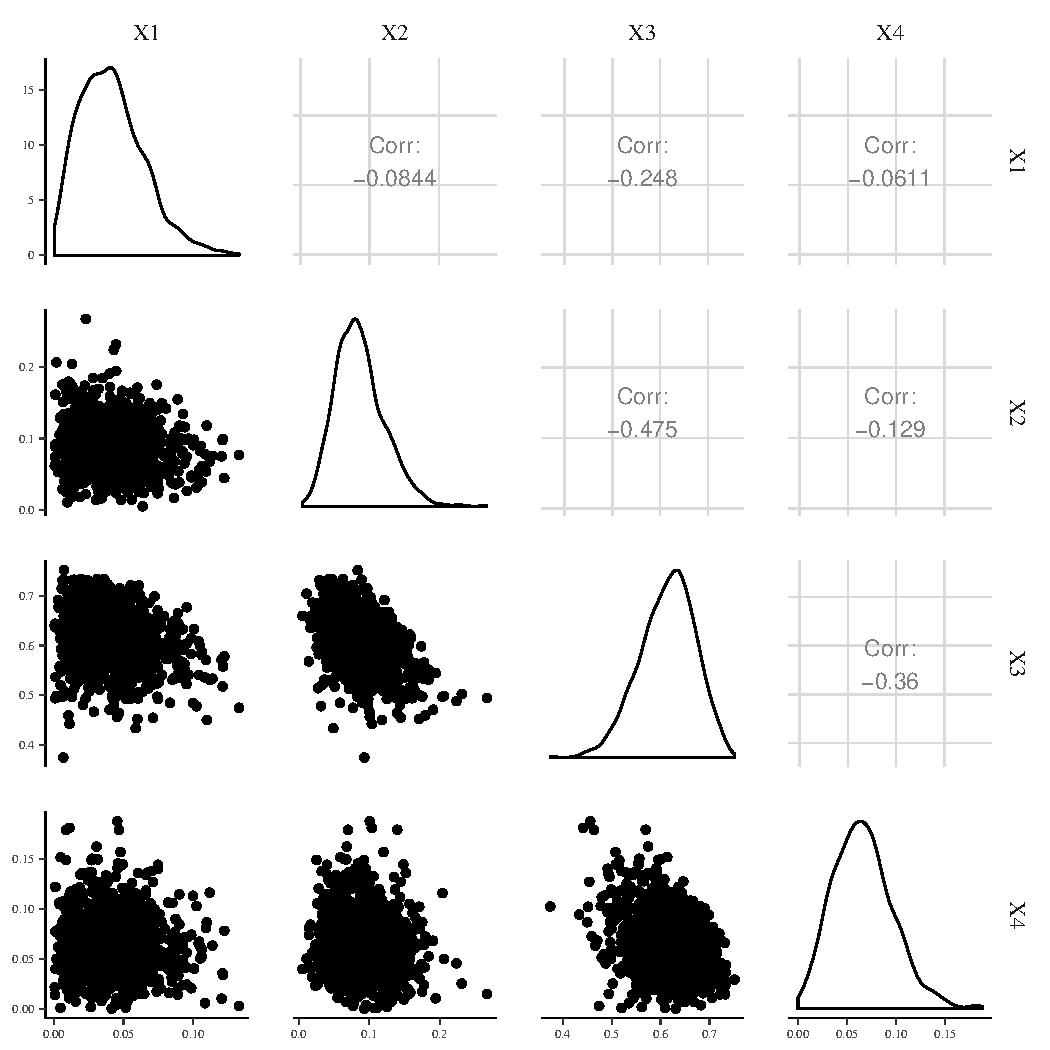
\includegraphics[width=\maxwidth]{figure/ch03_figsimdata_LMG_plot-1} \caption[Posterior distribution of LMG values]{Posterior distribution of LMG values.}\label{fig:simdata.LMG.plot}
\end{figure}


\end{knitrout}

\begin{table}[h]
\caption{Variance decomposition for non-stochastic predictors. I = LMG values, J = joint contribution, Total = total explained variance in one-predictor only model}
\centering
\begin{tabular}{clll}
  \toprule
  \multicolumn{1}{c}{\textbf{Variable}} & \multicolumn{1}{c}{\textbf{I}} &\multicolumn{1}{c}{\textbf{J}} & \multicolumn{1}{c}{\textbf{Total}} \\
  \hline
x1 & 0.039 (0.007, 0.094)  & 0.012 (0.004, 0.019)   & 0.051 (0.012, 0.113)  \\ 
x2 & 0.083 (0.03, 0.164)  & -0.022 (-0.032, -0.013)   & 0.06 (0.015, 0.133)  \\ 
x3 & 0.618 (0.497, 0.714)  & -0.02 (-0.031, -0.008)   & 0.598 (0.472, 0.697)  \\ 
x4 & 0.064 (0.014, 0.134)  & -0.001 (-0.002, \ensuremath{-3.301\times 10^{-4}})   & 0.063 (0.014, 0.133)  \\ 
   \bottomrule
\end{tabular}
\label{tbl:nonstochEx1}
\end{table}




\begin{table}[h]
\caption{Variance decomposition for non-stochastic predictors. I = LMG values, J = joint contribution, Total = total explained variance in one-predictor only model}
\centering
\begin{tabular}{cll}
   \toprule
   &\multicolumn{2}{c}{\textbf{LMG value (95\%-CI)}} \\
 \textbf{Variable} & \multicolumn{1}{c}{Relaimpo} & \textbf{Bayesian framework}  \\
  \hline
x1 & 0.092 (0.046, 0.157)  & 0.039 (0.007, 0.094)  \\ 
x2 & 0.109 (0.062, 0.177)  & 0.083 (0.03, 0.164)   \\ 
x3 & 0.636 (0.548, 0.723)  & 0.618 (0.497, 0.714)  \\ 
x4 & 0.03 (0.007, 0.072) & 0.064 (0.014, 0.134)  \\ 
   \bottomrule
\end{tabular}
\label{tbl:nonstochEx1relamip}
\end{table}

\FloatBarrier


In this example we know that the predictor values were sampled from a normal distribution. It would therefore be more reasonable to assume stochastic predictors. Under the assumption of weak exogeinity and conditional independence, the posterior distributions of the regression parameters $\bbeta$ are valid for non-stochastic and stochastic predictors. However, the uncertainty about the LMG values needs to include the uncertainty about the covariance matrix. If we know the distribution of the predictors we can incorporate this information and obtain the posterior distribution of the covariance matrix. The package \texttt{Jags} was used for inference about the covariance matrix in a Bayesian way. As an alternative non-parametric bootstrap was used for inference about the covariance matrix. Both approaches resulted in very similar LMG values. Using the default priors further resulted in very similar LMG values as the non-parametric bootstrap option of the relaimpo package. Table~\ref{tbl:nonstochEx1relaimpstoch} shows the LMG values of these approaches. Using the bootstrap samples of the covariance matrix or samples from the posterior covariance matrix resulted in very similar LMG values. Bootstrap seems to be a valuable option for stochastic predictors when the distribution of the predictors is unknown. Even when the distribution is known, the difference seems to be tiny. A benefit of going the full Bayesian way is that we can also include prior knowledge about the covariance matrix. For stochastic predictors, compared to non-stochastic predictors, the uncertainty about the covariance matrix is reflected in the larger credible intervals . Even when we would knew the exact regression parameters, there is a lot of uncertainty in the LMG values caused by the uncertainty about the covariance matrix. 








\begin{table}[h]
\caption{LMG values assuming stochastic predictors with 95\% CI.}
\centering
\begin{tabular}{clll}
   \toprule
  & \multicolumn{1}{c}{\textbf{Relaimpo}} & \multicolumn{2}{c}{\textbf{Bayesian framework}} \\ \cmidrule(r){2-2}\cmidrule(l){3-4}
 \textbf{Variable} &  & \multicolumn{1}{c}{nonparameteric bootstrap}& \multicolumn{1}{c}{covariance inference} \\
 \midrule
x1 & 0.092 (0.02, 0.221)  & 0.047 (0.005, 0.144) &  0.078 (0.018, 0.17) \\ 
x2 & 0.109 (0.026, 0.241)  & 0.15 (0.055, 0.279)  & 0.156 (0.052, 0.273) \\ 
x3 & 0.636 (0.452, 0.757)  & 0.554 (0.395, 0.71)  & 0.561 (0.442, 0.66) \\ 
x4 & 0.03 (0.008, 0.11) & 0.034 (0.008, 0.097) & 0.033 (0.011, 0.103) \\ 
   \bottomrule
\end{tabular}
\label{tbl:nonstochEx1relaimpstoch}
\end{table}







\clearpage

\section{Empirical Data}
In the following section, the Bayesian LMG implementation is applied on an empirical dataset containing test scores of pupils (N = 301) from a study by \cite{Holzinger1939} available in the R package \texttt{MBESS} \citep{MBESS}. This dataset was used in \cite{Nimon2008} to present commonality analysis, which is another variance decomposition technique. Scores from a paragraph comprehension test (paragrap) was predicted by four verbal tests:  general-information (general),  sentence-comprehension (sentence) ,  word-classification (wordc), and  word-meaning (wordm) (Table~\ref{table:hs.data}). 

The aim of the regression analysis  was to determine the strength of association between verbal ability and paragraph comprehension.  
An overview of the data is shown in Figure~\ref{fig:empi.lmg.plot}. The regression results of the paragraph comprehension scores on the verbal test scores are shown Table~\ref{tbl:empirical.reg}). A novice researcher may wrongly conclude, that there is little association between the \textit{non-significant} predictors (general information and word classification) and paragraph comprehension. Given the other predictors are already included in the model, the predictors seem not to provide us much information about the expected paragraph comprehension ability. However, we can not conclude out of this regression table, that the association between any of these \textit{non-significant} predictors and the dependent variable is unimportant. We see in Figure~\ref{fig:empi.lmg.plot} that the correlations between the predictors is rather high. The LMG metric may therefore provide us some new information about the importance of each predictor. 

The Bayesian regression model was fitted in \texttt{rstanarm}. The default priors were used for the regression coefficients and the $\sigma^2$ parameter. A burn-in period of 20000, a sample size of 20000 and a thinning of 20 resulted in a posterior sample size of 1000. The first few posterior samples are shown in Table~\ref{tab:empirical.data.postsample2}. The resulting $\Rtwo$ of of these posterior samples is shown in Table~\ref{tab:empirical.data.postsample3}. The LMG values were calculated by using \texttt{hier.part}. The  independent component (I), joint contribution (J) and total explained variance in a predictor-only model (T) are shown in Table~\ref{tbl:empirical.ijt}. Sentence-comprehension and word-meaning seem to be the most important predictors by the LMG metric. However, none of the predictors seem to be unimportant.  The joint contributions of each predictor is quite large.

For comparison purposes, the LMG metric was additionally calculated with the \texttt{relaimpo} package using parametric bootstrapping. The confidence intervals of  \texttt{relaimpo} are almost identical to the credible intervals of the Bayesian framework (Table~\ref{tbl:empirical.relaimp.comp}). Assuming stochastic or non-stochastic predictors would also result in almost identical uncertainty estimates with such a large sample size (Table\ref{tbl:empirical.relaimp.comp.stoch}). 







\begin{table}
\centering
\caption{Variable description}
\begin{tabular}{l l}
  \toprule			
  Variable Name & Description  \\   \midrule  
  paragrap & scores on paragraph comprehension test  \\
  general & scores on general information test \\
  sentence & scores on sentence completion test\\
  wordc & scores on word classification test \\
  wordm & scores on word meaning test \\
  \bottomrule  
\end{tabular}
\label{table:hs.data}
\end{table}

\begin{figure}
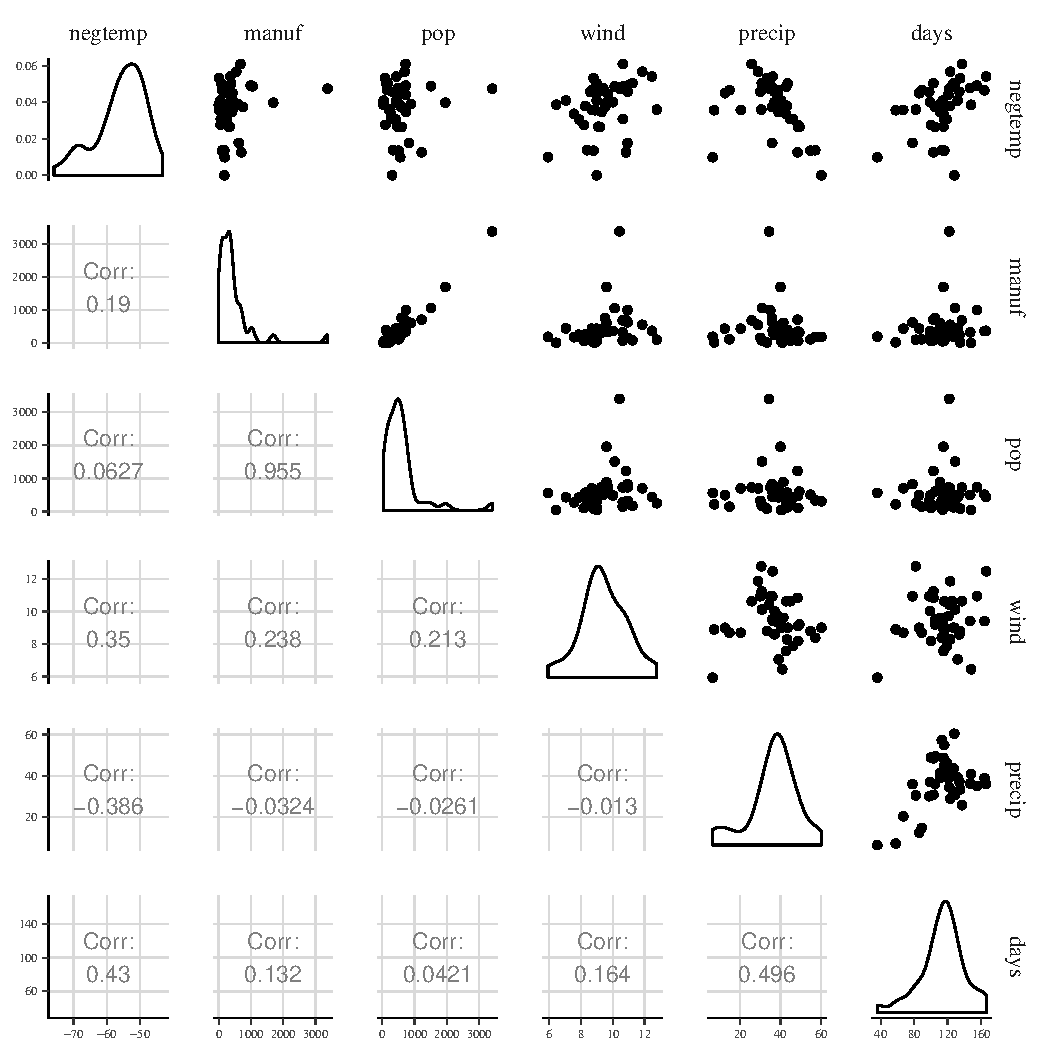
\includegraphics[width=\maxwidth]{figure/ch03_figunnamed-chunk-1-1} \caption[Test scores from Holzinger and Swineford's  (1939) Study]{Test scores from Holzinger and Swineford's  (1939) Study. N=301}\label{fig:unnamed-chunk-1}
\end{figure}






% latex table generated in R 3.4.3 by xtable 1.8-2 package
% Mon Aug  6 18:29:06 2018
\begin{table}[!h]
\centering
\caption{Regression of paragraph comprehension on verbal tests.} 
\label{tbl:empirical.reg}
\begingroup\footnotesize
\begin{tabular}{rrrr}
  \hline
 & Coefficient & 95\%-confidence interval & $p$-value \\ 
  \hline
Intercept & 0.071 & from -1.17 to 1.31 & 0.91 \\ 
  general & 0.03 & from -0.00 to 0.06 & 0.084 \\ 
  sentence & 0.26 & from 0.18 to 0.34 & $<$ 0.0001 \\ 
  wordc & 0.047 & from -0.01 to 0.11 & 0.14 \\ 
  wordm & 0.14 & from 0.08 to 0.19 & $<$ 0.0001 \\ 
   \hline
\end{tabular}
\endgroup
\end{table}


\begin{knitrout}
\definecolor{shadecolor}{rgb}{0.969, 0.969, 0.969}\color{fgcolor}\begin{table}

\caption{\label{tab:empirical.data.postsample2}Samples from the posterior distributions of the regression parameters}
\centering
\begin{tabular}[t]{lrrrrr}
\toprule
  & general & sentence & wordc & wordm & sigma\\
\midrule
sample 1 & 0.041 & 0.270 & 0.014 & 0.113 & 2.18\\
sample 2 & 0.036 & 0.243 & 0.010 & 0.166 & 2.09\\
sample 3 & 0.043 & 0.295 & -0.007 & 0.103 & 2.28\\
sample 4 & 0.024 & 0.240 & 0.051 & 0.192 & 2.19\\
sample 5 & 0.050 & 0.297 & 0.009 & 0.099 & 2.28\\
sample 6 & 0.027 & 0.259 & 0.040 & 0.157 & 2.09\\
sample 7 & 0.029 & 0.265 & 0.023 & 0.156 & 2.11\\
sample 8 & 0.017 & 0.259 & 0.026 & 0.168 & 2.18\\
sample 9 & 0.036 & 0.250 & 0.073 & 0.123 & 2.00\\
sample 10 & 0.004 & 0.269 & 0.059 & 0.163 & 2.10\\
\bottomrule
\end{tabular}
\end{table}


\end{knitrout}

\begin{knitrout}
\definecolor{shadecolor}{rgb}{0.969, 0.969, 0.969}\color{fgcolor}\begin{table}

\caption{\label{tab:empirical.data.postsample3}$ \Rtwo$ for all submodels for the first six posterior samples}
\centering
\begin{tabular}[t]{lrrrrrr}
\toprule
  & sample 1 & sample 2 & sample 3 & sample 4 & sample 5 & sample 6\\
\midrule
none & 0.000 & 0.000 & 0.000 & 0.000 & 0.000 & 0.000\\
general & 0.426 & 0.455 & 0.407 & 0.449 & 0.433 & 0.448\\
sentence & 0.520 & 0.537 & 0.508 & 0.541 & 0.527 & 0.554\\
wordc & 0.299 & 0.312 & 0.271 & 0.348 & 0.298 & 0.343\\
wordm & 0.462 & 0.542 & 0.433 & 0.559 & 0.446 & 0.534\\
general sentence & 0.558 & 0.583 & 0.541 & 0.583 & 0.566 & 0.592\\
general wordc & 0.455 & 0.482 & 0.428 & 0.493 & 0.459 & 0.490\\
general wordm & 0.511 & 0.578 & 0.482 & 0.588 & 0.504 & 0.569\\
sentence wordc & 0.527 & 0.545 & 0.511 & 0.557 & 0.533 & 0.567\\
sentence wordm & 0.574 & 0.627 & 0.551 & 0.640 & 0.571 & 0.633\\
wordc wordm & 0.497 & 0.568 & 0.462 & 0.595 & 0.484 & 0.573\\
general sentence wordc & 0.559 & 0.583 & 0.541 & 0.587 & 0.566 & 0.595\\
general sentence wordm & 0.583 & 0.634 & 0.560 & 0.644 & 0.583 & 0.638\\
general wordc wordm & 0.523 & 0.587 & 0.490 & 0.606 & 0.516 & 0.588\\
sentence wordc wordm & 0.576 & 0.628 & 0.552 & 0.645 & 0.572 & 0.636\\
all & 0.584 & 0.634 & 0.560 & 0.647 & 0.583 & 0.640\\
\bottomrule
\end{tabular}
\end{table}


\end{knitrout}



\begin{knitrout}
\definecolor{shadecolor}{rgb}{0.969, 0.969, 0.969}\color{fgcolor}\begin{figure}
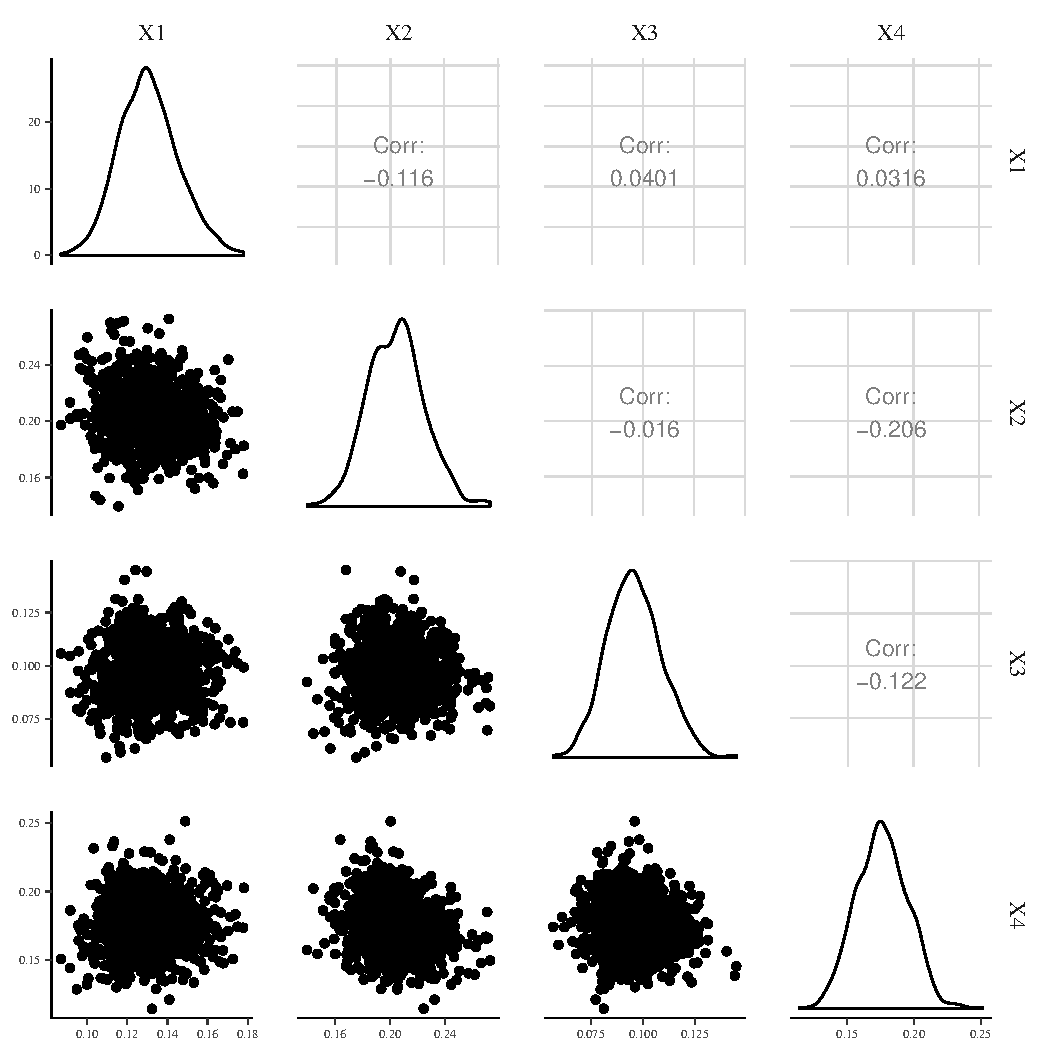
\includegraphics[width=\maxwidth]{figure/ch03_figempi_lmg_plot-1} \caption[LMG posterior distribution of different verbal ability tests]{LMG posterior distribution of different verbal ability tests}\label{fig:empi.lmg.plot}
\end{figure}


\end{knitrout}


\begin{table}[h]
\caption{Variance decomposition for non-stochastic predictors. I = LMG values, J = joint contribution, Total = total explained variance in one-predictor only model}
\centering
\begin{tabular}{clll}
  \toprule
  \multicolumn{1}{c}{\textbf{Variable}} & \multicolumn{1}{c}{\textbf{I}} &\multicolumn{1}{c}{\textbf{J}} & \multicolumn{1}{c}{\textbf{Total}} \\
  \hline
general & 0.13 (0.105, 0.16)  & 0.299 (0.258, 0.333)   & 0.429 (0.364, 0.489)  \\ 
sentence & 0.203 (0.165, 0.245)  & 0.328 (0.293, 0.355)   & 0.532 (0.465, 0.588)  \\ 
wordc & 0.096 (0.073, 0.128)  & 0.24 (0.2, 0.275)   & 0.336 (0.273, 0.401)  \\ 
wordm & 0.176 (0.138, 0.214)  & 0.315 (0.278, 0.344)   & 0.492 (0.421, 0.55)  \\ 
   \bottomrule
\end{tabular}
\label{tbl:empirical.ijt}
\end{table}


\begin{table}[h]
\caption{Variance decomposition for non-stochastic predictors. I = LMG values, J = joint contribution, Total = total explained variance in one-predictor only model}
\centering
\begin{tabular}{cll}
   \toprule
   &\multicolumn{2}{c}{\textbf{LMG value (95\%-CI)}} \\
 \textbf{Variable} & \multicolumn{1}{c}{Relaimpo} & \textbf{Bayesian framework}  \\
  \hline
general & 0.131 (0.106, 0.161)  & 0.13 (0.105, 0.16)  \\ 
sentence & 0.206 (0.168, 0.251)  & 0.203 (0.165, 0.245)   \\ 
wordc & 0.096 (0.073, 0.125)  & 0.096 (0.073, 0.128)  \\ 
wordm & 0.178 (0.141, 0.219) & 0.176 (0.138, 0.214)  \\ 
   \bottomrule
\end{tabular}
\label{tbl:empirical.relaimp.comp}
\end{table}





\begin{table}[h]
\caption{Variance decomposition for Stochastic predictors. I = LMG values, J = joint contribution, Total = total explained variance in one-predictor only model}
\centering
\begin{tabular}{cll}
   \toprule
   &\multicolumn{2}{c}{\textbf{LMG value (95\%-CI)}} \\
 \textbf{Variable} & \multicolumn{1}{c}{Relaimpo} & \textbf{Bayesian framework}  \\
  \hline
general & 0.131 (0.106, 0.163)  &  0.127 (0.092, 0.16)  \\ 
sentence & 0.206 (0.171, 0.246)  &  0.204 (0.163, 0.249)   \\ 
wordc & 0.096 (0.075, 0.128)  &  0.097 (0.07, 0.128)  \\ 
wordm & 0.178 (0.144, 0.218) &  0.175 (0.136, 0.214) \\ 
   \bottomrule
\end{tabular}
\label{tbl:empirical.relaimp.comp.stoch}
\end{table}


% LaTeX file for Chapter 04





\chapter{Extension of the LMG formula for longitudinal data}

In the following chapter some extenstions of the LMG formula beyond the simple linear regression model are shown. The focus is on repeated measurements models. These models extend the simple linear regression by allowing intra subject correlation between repeated measures.

The dependence within subjects can be modeled by including random effects (mixed model) or by assuming correlated errors within a subject (marginal model). Using a random intercept model or a compound symmetry matrix for the error will result in the same fixed effect estimate. A mixed model can be extended by including a random slope per subject, allowing for less restrictive longitudinal shapes. The marginal approach can get more freedom by different specified covariance matrices of the error terms. An unstructured covariance matrix, where no restriction are imposed, allows for the most freedom. However, depending on the number of repeated measuresments and the sample size the covariance matrix can get too large to make reasonable inference about it. 

The extenstion of the LMG formula in the Bayesian framework to longitudinal models is restricted to models where the conditional variance formula can  be applied to get the explained variance of the submodel from the regression parameters of the full model. The focus is therefore on the fixed predictors and not on the random effects. The conditional variance formula can be used in the marginal models, where only the fixed effects are modelled anyway. In the mixed model framework, the conditional variance formula is applicable to random intercepts models. For random-slope models there are atleast some difficulties involved, if it is possible at all, to get the explained variance of the submodel. This chapter shows the Bayesian LMG Implementation on a random intercept model and on a repeated measurement model with an unstructured covariance matrix.  


\section{random intercept model}
The first example concerns a simple random intercept model with time varying predictors.  Different $\Rtwo$ metrics exist for linear mixed models \citep{Nakagawa2013}. The variance of a random intercept model with regression parameter $\bbeta$ can be written as

      \begin{align} 
        \var(y) = \sigma_{f}^2  + \sigma_{\alpha}^2 + \sigma_{\epsilon}^2, \label{eq:var.t.ri} 
        \end{align}

where $\sigma_{f}^2 = \var(\X \bbeta) = \bbeta^\top \bSigma_{\X \X}  \bbeta$ , $\sigma_{\alpha}^2 $ is the random intercept and $\sigma_{\epsilon}^2$ is the error term. 

An $\Rtwo$ that is guaranteed to be positive is defined in \cite{Nakagawa2013} as

   \begin{align} 
\Rtwo_{\text{LMM}} = \frac{\sigma_{f}^2}{\sigma_{f}^2 + \sigma_{\alpha}^2 + \sigma_{\epsilon}^2},
\end{align}


 It is theoretically possible that the $\Rtwo_{\text{LMM}}$ decreases when adding predictors \citep{Nakagawa2013}.  By adding predictors $\sigma_{f}^2$  should always increase and  $\sigma_{\epsilon}^2$  decrease. However, the $\sigma_{\alpha}^2$ may also increase a little bit and the total $\Rtwo$ may then be a little bit lower. The $\Rtwo$ can not decrease by using the conditional variance formula on the full model to calculate the $\Rtwo$ of the submodels because the total variance is fixed. The results will be the same as if we would fit a new model by maximum likelihood for each submodel and only compare the variance of the fixed effects to the explained variance of the full model.  In the Bayesian framework we need the conditional variance formula to account for the interdepdence of the submodels to each other. The total variance of the full model can be calculated as  $\var(y) = \var(\X \bbeta + \Z b) + \sigma^2$ or by using samples of $\sigma_{\alpha}^2$ as in \eqref{eq:var.t.ri}. The error term could again be sampled or calculated as in \eqref{rtwoGelman}. In the following examples, \eqref{eq:var.t.ri} is used and  $\sigma_{\alpha}^2$ and $\sigma_{\epsilon}^2$ are sampled from their posterior distribution.

In repeated measurement studies the focus is often in within-subject changes. The between subject variance estimated with the random intercept term is of minor importance. The more important question may be how much the fixed predictors explain compared to the within subject error, which is

   \begin{align} 
\Rtwo_{\text{repeated}} = \frac{\sigma_{f}^2}{\sigma_{f}^2  + \sigma_{\epsilon}^2}, \label{rtwo.repeated}
\end{align}

The square root of this term is known under the name correlation within subjects in \cite{Bland1995}. Often, there are between-subject and within-subject predictors in a model. If we are interested in the within-subject effect, we can use a model including only the between-subject predictors as the null-model.

The following example shows a simple random intercept model with time-varying predictors. The main question is which within-subject predictors are the most important ones. The between-subject variance is of minor importance. 

The data are simulated from the following regression setting with $m = 4$ timepoints and $n = 20$ number of subjects ,

\begin{align*} 
Y_{i,j} \sim \mathcal{N}(\beta_{0}+x_{1_{i,j}} \beta_{1}+x_{2_{i,j}} \beta_{2}+x_{3_{i,j}} \beta_{3}+x_{4_{i,j}} \beta_{4} + \alpha_{i}, \, \sigma^2), \qquad &i = 1, \dots, n \\  &j = 1, \dots, m
\end{align*} 

where $\beta_{1} = 1 \,$,  $\beta_{2} = 1 \,$,   $\beta_{3} = 2 \,$  $\beta_{4}=2 \,$, $\sigma^2 = 1 \, $, $\alpha_{i} \sim \mathcal{N}(0, \sigma_{\alpha}^2) \,$, $\X \sim \mathcal{N}(\0, \bSigma)$.

The R code can be found in the appendix:



\begin{knitrout}
\definecolor{shadecolor}{rgb}{0.969, 0.969, 0.969}\color{fgcolor}\begin{figure}
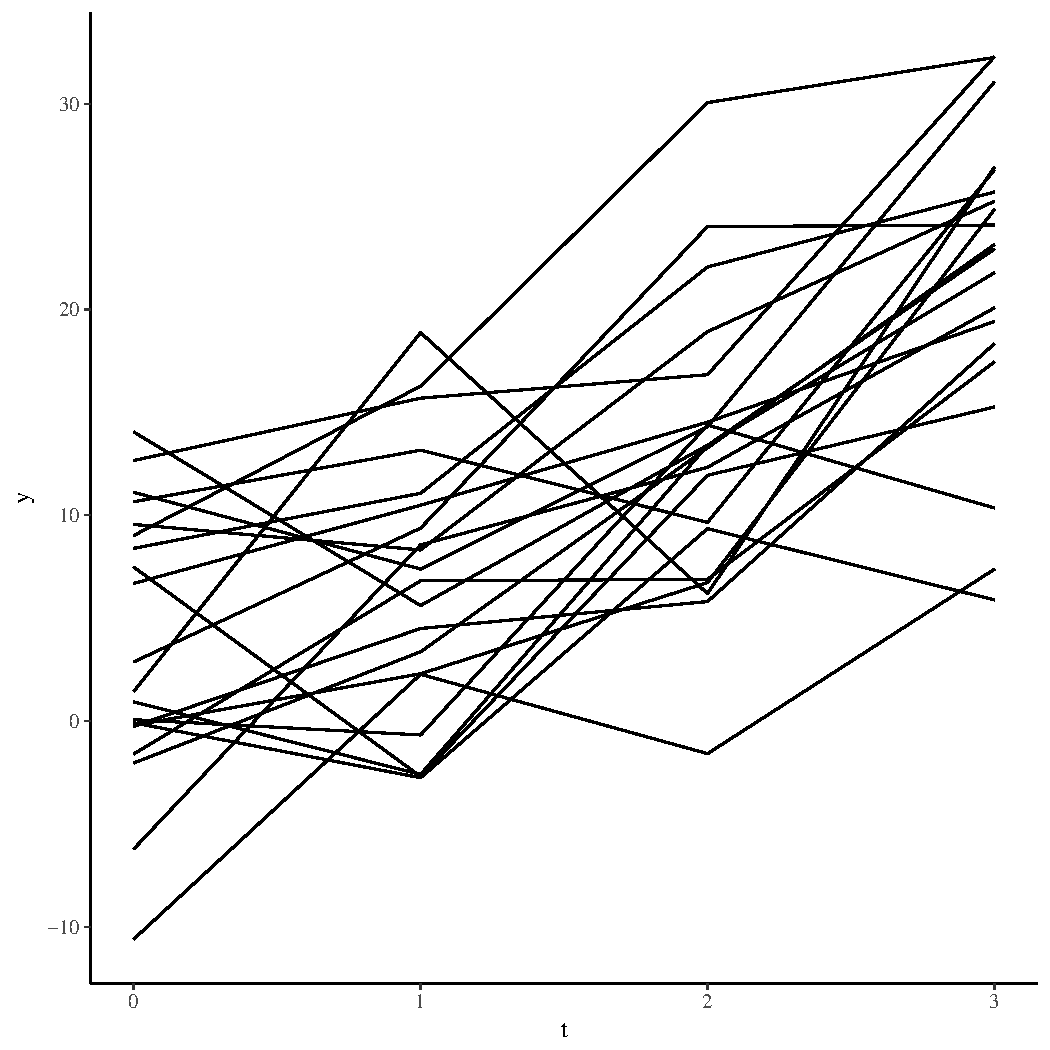
\includegraphics[width=\maxwidth]{figure/ch04_fig_repeated_plot_ri-1} \caption[Individual trajectories of simulated random intercept model]{Individual trajectories of simulated random intercept model}\label{fig:.repeated.plot.ri}
\end{figure}


\end{knitrout}


The random intercept effect is not of interest. The $\Rtwo$ of the models is calculated according to the formula of repeated measure correlation \eqref{rtwo.repeated}.  Most of the within subject variance is explained by the predictors (Table~\ref{tbl:repeatedcormod}). The credible intervals are very narrow. For the information about the between subject varinace could look at the random intercept variance directly. 

In the second part the random intercept is dirctly included in the total variance calculation of the $\Rtwo$ values. There is a large between-subject variance in this dataset (Table~\ref{tbl:repeatedcormod.tot}). The LMG values including the between subject variance are much lower. The credible intervals are also much wider, because the uncertainty about the between-subject variance is included. 

In my opinion we can get more useful infromation from separating the between and within variance components when it is easy possible. Note that we assumed non stochastic predictors. Otherwise, the credible intervals would be larger. In general, it seems more reasonable to assume stochastic time-varying predictors. The variance could then be estimated by non-parameteric bootstrap, resampling whole subjects (all repeated measurements of a subject).





\begin{table}[h]
\caption{Variance decomposition for non-stochastic predictors. I = LMG values, J = joint contribution, Total = total explained variance in one-predictor only model}
\centering
\begin{tabular}{clll}
  \toprule
  \multicolumn{1}{c}{\textbf{Variable}} & \multicolumn{1}{c}{\textbf{I}} &\multicolumn{1}{c}{\textbf{J}} & \multicolumn{1}{c}{\textbf{Total}} \\
  \hline
x1 & 0.202 (0.2, 0.203)  & 0.525 (0.523, 0.526)   & 0.727 (0.723, 0.73)  \\ 
x2 & 0.21 (0.208, 0.211)  & 0.538 (0.536, 0.539)   & 0.747 (0.744, 0.751)  \\ 
x3 & 0.297 (0.296, 0.299)  & 0.658 (0.658, 0.658)   & 0.955 (0.954, 0.957)  \\ 
x4 & 0.291 (0.29, 0.292)  & 0.651 (0.65, 0.651)   & 0.942 (0.94, 0.943)  \\ 
   \bottomrule
\end{tabular}
\label{tbl:repeatedcormod}
\end{table}




\begin{table}[h]
\caption{Variance decomposition for non-stochastic predictors. I = LMG values, J = joint contribution, Total = total explained variance in one-predictor only model}
\centering
\begin{tabular}{clll}
  \toprule
  \multicolumn{1}{c}{\textbf{Variable}} & \multicolumn{1}{c}{\textbf{I}} &\multicolumn{1}{c}{\textbf{J}} & \multicolumn{1}{c}{\textbf{Total}} \\
  \hline
x1 & 0.108 (0.046, 0.172)  & 0.238 (0.116, 0.35)   & 0.346 (0.163, 0.522)  \\ 
x2 & 0.089 (0.046, 0.127)  & 0.229 (0.116, 0.329)   & 0.318 (0.162, 0.456)  \\ 
x3 & 0.113 (0.06, 0.161)  & 0.272 (0.139, 0.391)   & 0.385 (0.199, 0.551)  \\ 
x4 & 0.115 (0.061, 0.163)  & 0.27 (0.137, 0.387)   & 0.385 (0.199, 0.55)  \\ 
   \bottomrule
\end{tabular}
\label{tbl:repeatedcormod.tot}
\end{table}



\section{marginal  model}

The next example concerns a repeated measurement model with time-varying predictors an unstructured covariance error covariance matrix. The data are generated from the following model:

\begin{align} 
&Y_{i} \sim \mathcal{N}(\X_{i} \bbeta, \bSigma), \qquad i = 1, \dots, n
\end{align} 

where $\bSigma$ represents an unstructured error covariance matrix, $\X_{i}$ represents the predictor matrix of subject $i$.

In the variance calculation we need to take into account that we do not have just one $\sigma^2$ parameter, but a covariance matrix $\bSigma$. The diagonal elements of $\bSigma$ represent the variance of each timepoint. The sum of the diagonal elements of $\bSigma$ represents the variance for a whole subject. When there are no missing timepoints in each subject, we can  take the mean of $\diag(\bSigma)$ to make the formula compatiable with the $\bbeta^\top \bSigma_{\X \X}  \bbeta$ of \eqref{rtwoused}, resulting in the total variance term

      \begin{align} 
        \var(\Y) = \bbeta^\top \bSigma_{\X \X}  \bbeta + \text{mean}(\diag(\bSigma)),
   \end{align}

The following R-code is used to generate the data:



\begin{knitrout}
\definecolor{shadecolor}{rgb}{0.969, 0.969, 0.969}\color{fgcolor}\begin{figure}
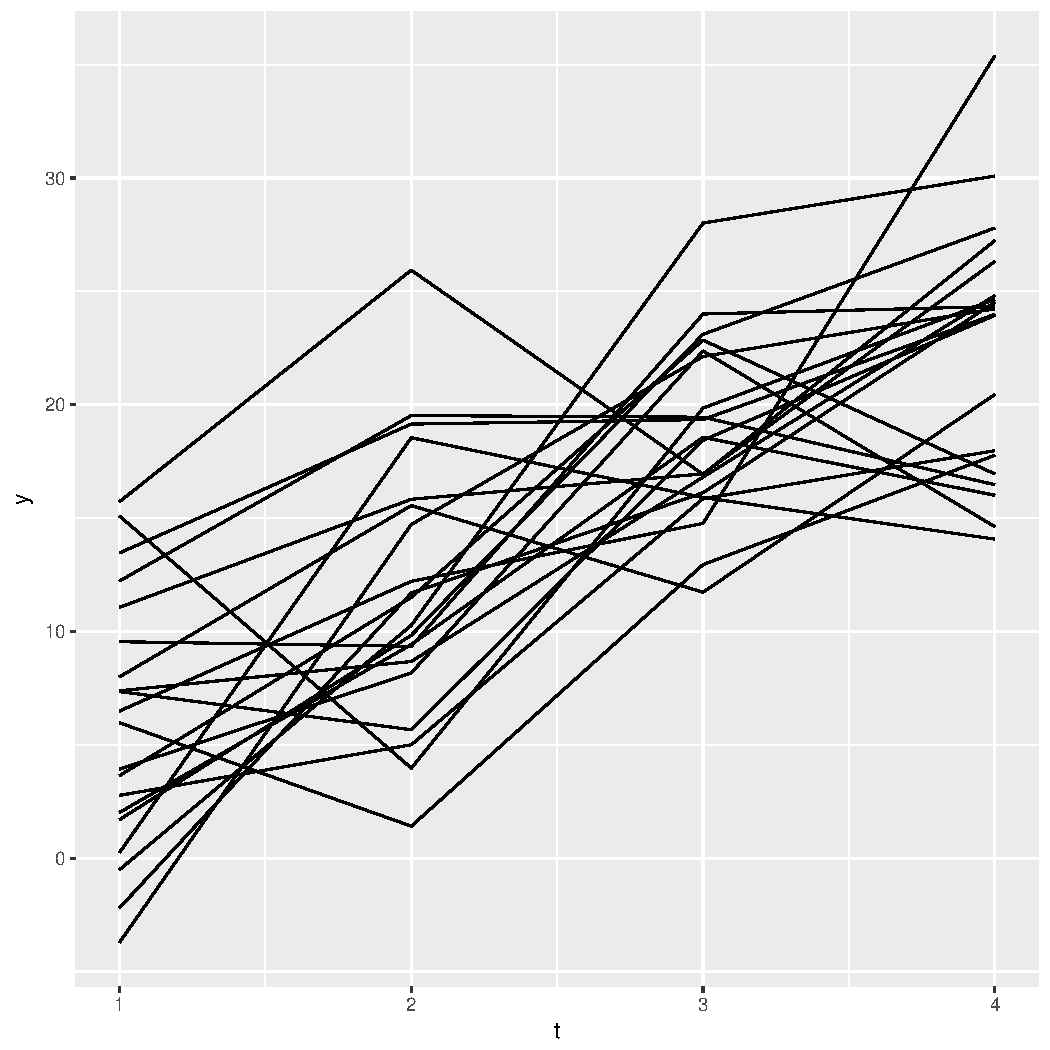
\includegraphics[width=\maxwidth]{figure/ch04_figsimdata_repeated_unstruct_plot-1} \caption[Individual trajectories of simulated data with unstructured error covariance matrix]{Individual trajectories of simulated data with unstructured error covariance matrix}\label{fig:simdata.repeated.unstruct.plot}
\end{figure}


\end{knitrout}




The individual trajectories are shown in Figure~\ref{fig:simdata.repeated.unstruct.plot}. The resulting LMG values of the predictors are shown in Table \ref{tbl:repeated.unstructured}.

\begin{table}[h]
\caption{Variance decomposition for non-stochastic predictors. I = LMG values, J = joint contribution, Total = total explained variance in one-predictor only model}
\centering
\begin{tabular}{clll}
  \toprule
  \multicolumn{1}{c}{\textbf{Variable}} & \multicolumn{1}{c}{\textbf{I}} &\multicolumn{1}{c}{\textbf{J}} & \multicolumn{1}{c}{\textbf{Total}} \\
  \hline
x1 & 0.141 (0.113, 0.163)  & 0.364 (0.299, 0.406)   & 0.506 (0.413, 0.568)  \\ 
x2 & 0.137 (0.11, 0.16)  & 0.353 (0.292, 0.395)   & 0.49 (0.405, 0.554)  \\ 
x3 & 0.206 (0.168, 0.233)  & 0.443 (0.366, 0.489)   & 0.65 (0.537, 0.719)  \\ 
x4 & 0.21 (0.172, 0.239)  & 0.444 (0.367, 0.489)   & 0.656 (0.543, 0.725)  \\ 
   \bottomrule
\end{tabular}
\label{tbl:repeated.unstructured}
\end{table}





% LaTeX file for Chapter 05






\chapter{Other variable importance metrics in the Bayesian framework}

Different variable importance metrics exist. The conditional variance formula allowed us to calculate the $\Rtwo$ of the submodels from the posterior sample of the full model. The focus of this master thesis was on the LMG formula. For each posterior sample the LMG formula can be applied for the submodels of each posterior sample. A lot of the variable importance metrics are based on the $\Rtwo$ of the full model compared to the submodels. Instead of the LMG formula we could as well have used another variable importance metric after we have calculated the $\Rtwo$ of all the submodels. Commonality and dominance analysis seem to be interesting extensions of the LMG framework. Both provide besides the LMG information some other information about the variance decomposition of the predictors. The relaimpo package provides some more bootstrap options like pariwise differences that could also be easily transfered to the Bayesian framework. 


 
\section{Conclusion}

The Bayesian framworks provides us with a nice option to include the uncertainty about parameters. Posterior distributions of the parameters allow us to calculate a distribution of $\Rtwo$ values for each model. Using  the conditional variance formula allowd us to calculate the $\Rtwo$ of all the submodels from the posterior parameter distributions of the full model. Instead of fitting $2^
{p-1}$ models, only the full model needs to be fitted. Doing it this way has some nice properties. The interdependence of the submodels to each other is respected. The $\Rtwo$ of the submodels does not decrease when adding predictors. The non-negativity of the shares is therefore respected in the LMG formula. This property of using the conditional variance formula is also interesting when the LMG formula is applied to random intercept models fitted by maximum likelihood. 

A disadventage about calculating the $\Rtwo$ of all the submodels with the conditional variance formula  seems to be the restriction to the linear model. Although this may be a topic of further research.

Assuming non-stochastic or stochastic predictors can have a big impact on the the uncertainty of the explained variance and the LMG values. Although the posterior regression parameter distribtuions is the same in both cases (under some assumptions described in chapter ...) the explainened variance of a model is directly dependent on the covarinace matrix. Inference about the covariance of the predictors $\X$ is therefore an important part when stochastic predictors are assumed. However, this does in general not seem to be an easy problem. Non-parametric bootstrap provides a practical solution. 




% LaTeX file for appendix






\chapter{Appendix}

he eror term in the by \cite{Gelman2017} proposed definition of the $\Rtwo$ is defined as $\var(\sum_{i=1}^{n}e^s_{n})$. I think we could also use $ \sum(y - \hat{y}^s)^2/(n-1) $ as an estimate for the error. For the maximum likelihood estimate $\var(y_{i} - \hat{y_{i}}) = \sum (y_{i} - \hat{y_{i}})^2/ (n-1) $. This is because the mean of the residuals is 0. When  samples of the posterior parameters are used, the mean of the residuals is not excatly zero. $\var(y_{i} - \hat{y_{i}}) = \sum (y_{i} - \hat{y_{i}})^2/ (n-1) $ is than a little bit bigger than $\var(y_{i} - \hat{y_{i}}). $ In practice the values should only differ by a very small amount. We do not expect the errors to have a systematic bias. However, the residuals are just a sample of the error. The mean of the residuals must not be excatly 0 when the samples of the posteriors are used for the regression coefficients.   




\cleardoublepage

\appendix
\chapter{Formula}
\begin{knitrout}
\definecolor{shadecolor}{rgb}{0.969, 0.969, 0.969}\color{fgcolor}\begin{kframe}
\begin{alltt}
\hlkwd{set_parent}\hlstd{(}\hlstr{'Main.Rnw'}\hlstd{)}
\hlkwd{library}\hlstd{(knitr)}
\hlstd{opts_chunk}\hlopt{$}\hlkwd{set}\hlstd{(}
    \hlkwc{fig.path}\hlstd{=}\hlstr{'figure/ch01_fig'}\hlstd{,}
    \hlkwc{self.contained}\hlstd{=}\hlnum{FALSE}\hlstd{,}
    \hlkwc{cache}\hlstd{=}\hlnum{TRUE}
\hlstd{)}

\hlkwd{set_parent}\hlstd{(}\hlstr{'Main.Rnw'}\hlstd{)}
\hlkwd{library}\hlstd{(knitr)}
\hlstd{opts_chunk}\hlopt{$}\hlkwd{set}\hlstd{(}
    \hlkwc{fig.path}\hlstd{=}\hlstr{'figure/ch02_fig'}\hlstd{,}
    \hlkwc{self.contained}\hlstd{=}\hlnum{FALSE}\hlstd{,}
    \hlkwc{cache}\hlstd{=}\hlopt{!}\hlnum{FALSE}
\hlstd{)}
\hlkwd{set_parent}\hlstd{(}\hlstr{'Main.Rnw'}\hlstd{)}
\hlkwd{library}\hlstd{(knitr);} \hlkwd{library}\hlstd{(hier.part);} \hlkwd{library}\hlstd{(rstanarm);}  \hlkwd{library}\hlstd{(GGally);} \hlkwd{library}\hlstd{(ggplot2);} \hlkwd{library}\hlstd{(relaimpo);} \hlkwd{library}\hlstd{(rjags);} \hlkwd{library}\hlstd{(corpcor);} \hlkwd{library}\hlstd{(brinla);} \hlkwd{library}\hlstd{(stargazer);} \hlkwd{library}\hlstd{(xtable);} \hlkwd{library}\hlstd{(kableExtra);} \hlkwd{library}\hlstd{(MBESS);} \hlkwd{library}\hlstd{(MASS);} \hlkwd{library}\hlstd{(biostatUZH)}


\hlstd{opts_chunk}\hlopt{$}\hlkwd{set}\hlstd{(}
    \hlkwc{fig.path}\hlstd{=}\hlstr{'figure/ch03_fig'}\hlstd{,}
    \hlkwc{self.contained}\hlstd{=}\hlnum{FALSE}\hlstd{,}
    \hlkwc{cache}\hlstd{=}\hlnum{TRUE}
\hlstd{)}

\hlkwd{options}\hlstd{(}\hlkwc{digits} \hlstd{=}\hlnum{3}\hlstd{)}
\hlcom{#function to calculate R2 data frame}
\hlstd{rtwos}\hlkwb{<-}\hlkwa{function}\hlstd{(}\hlkwc{X}\hlstd{,} \hlkwc{post.sample}\hlstd{)\{}
  \hlcom{# X: Predictor data as data frame}
  \hlcom{# post.sample: posterior sample as matrix (M[sample_i,]), last position should be sigma paramater. }

  \hlstd{X} \hlkwb{<-} \hlkwd{cov}\hlstd{(X)} \hlcom{#covariance matrix}

  \hlcom{#Prepare data frame and rownames by using the combn() function}

  \hlstd{lst} \hlkwb{<-} \hlkwd{list}\hlstd{()}

  \hlstd{pcan} \hlkwb{<-} \hlkwd{dim}\hlstd{(X)[}\hlnum{2}\hlstd{]}
  \hlstd{n} \hlkwb{<-} \hlstd{(}\hlnum{2}\hlopt{^}\hlstd{pcan)}\hlopt{-}\hlnum{1}

  \hlkwa{for} \hlstd{(i} \hlkwa{in} \hlnum{1}\hlopt{:}\hlstd{pcan)\{}
    \hlstd{lst[[i]]} \hlkwb{<-} \hlkwd{combn}\hlstd{(pcan,i)}
  \hlstd{\}}

  \hlstd{var.names} \hlkwb{<-} \hlkwd{character}\hlstd{(}\hlkwc{length} \hlstd{=} \hlnum{0}\hlstd{)}

  \hlstd{v}\hlkwb{<-} \hlkwd{rownames}\hlstd{(X)}

  \hlkwa{for}\hlstd{(i} \hlkwa{in} \hlnum{1}\hlopt{:}\hlkwd{length}\hlstd{(lst))}
  \hlstd{\{}

    \hlkwa{for} \hlstd{(j} \hlkwa{in} \hlnum{1}\hlopt{:}\hlkwd{ncol}\hlstd{(lst[[i]]))\{}
      \hlstd{cur}\hlkwb{<-} \hlstd{lst[[i]][,j]}
      \hlstd{name} \hlkwb{<-} \hlkwd{paste0}\hlstd{(v[}\hlopt{-}\hlstd{cur])}
      \hlstd{name} \hlkwb{<-} \hlkwd{paste}\hlstd{(name,} \hlkwc{collapse} \hlstd{=} \hlstr{" "}\hlstd{)}
      \hlstd{var.names} \hlkwb{<-} \hlkwd{c}\hlstd{(var.names, name)}
    \hlstd{\}}
  \hlstd{\}}

  \hlstd{var.names}\hlkwb{<-}\hlkwd{c}\hlstd{(}\hlkwd{rev}\hlstd{(var.names),} \hlstr{'all'}\hlstd{)}

  \hlstd{var.names[}\hlnum{1}\hlstd{]}\hlkwb{<-}\hlstr{'none'}

  \hlstd{size} \hlkwb{<-} \hlkwd{nrow}\hlstd{(post.sample)}  \hlcom{# how many samples}

  \hlstd{sig.posi} \hlkwb{<-} \hlkwd{ncol}\hlstd{(post.sample)}

  \hlstd{df.Rtwos}\hlkwb{<-}\hlkwd{data.frame}\hlstd{(}\hlkwd{matrix}\hlstd{(}\hlnum{0}\hlstd{,n}\hlopt{+}\hlnum{1}\hlstd{,size))}

  \hlkwd{row.names}\hlstd{(df.Rtwos)} \hlkwb{<-} \hlstd{var.names}

  \hlcom{########### fill in R^2 matrix, use posterior samples and calculate submodels according to the conditional expectation formula.}

  \hlstd{v} \hlkwb{<-} \hlnum{1}\hlopt{:}\hlkwd{dim}\hlstd{(X)[}\hlnum{2}\hlstd{]}

  \hlkwa{for} \hlstd{(s} \hlkwa{in} \hlnum{1}\hlopt{:}\hlstd{size)\{}

    \hlstd{sample.s} \hlkwb{<-} \hlstd{post.sample[s,}\hlopt{-}\hlstd{sig.posi]}

    \hlstd{Vtot} \hlkwb{<-} \hlstd{sample.s}\hlopt\hlstd{X}\hlopt\hlstd{sample.s}  \hlcom{#total explained variance}

    \hlstd{count}\hlkwb{=}\hlstd{n}

    \hlkwa{for}\hlstd{(i} \hlkwa{in} \hlnum{1}\hlopt{:}\hlstd{(}\hlkwd{length}\hlstd{(lst)}\hlopt{-}\hlnum{1}\hlstd{))}
    \hlstd{\{}

      \hlkwa{for} \hlstd{(j} \hlkwa{in} \hlnum{1}\hlopt{:}\hlkwd{ncol}\hlstd{(lst[[i]]))\{}
        \hlstd{cur} \hlkwb{<-} \hlstd{lst[[i]][,j]}
        \hlstd{set} \hlkwb{<-} \hlstd{v[}\hlopt{-}\hlstd{cur]}
        \hlstd{matr} \hlkwb{<-} \hlstd{X[cur, cur]} \hlopt{-} \hlstd{X[cur, set]}\hlopt\hlkwd{solve}\hlstd{(X[set, set])}\hlopt\hlstd{X[set, cur]}  \hlcom{#conditional expectation formula, how much variance is explained by the predictors that are not included in the model and that is not explained by other predictors}
        \hlstd{var.explain}\hlkwb{<-} \hlstd{sample.s[cur]}\hlopt\hlstd{matr}\hlopt\hlstd{sample.s[cur]}  \hlcom{#multiply by parameter sample}
        \hlstd{df.Rtwos[count,s]} \hlkwb{<-} \hlstd{Vtot} \hlopt{-} \hlstd{var.explain}
        \hlstd{count}\hlkwb{=}\hlstd{count}\hlopt{-}\hlnum{1}
      \hlstd{\}}
    \hlstd{\}}

    \hlstd{df.Rtwos[n}\hlopt{+}\hlnum{1}\hlstd{,s]} \hlkwb{<-} \hlstd{Vtot}

    \hlstd{df.Rtwos[,s]} \hlkwb{<-} \hlstd{df.Rtwos[,s]}\hlopt{/}\hlkwd{c}\hlstd{(Vtot}\hlopt{+}\hlstd{post.sample[s,sig.posi]}\hlopt{^}\hlnum{2}\hlstd{)} \hlcom{#total variance + sigma^2 (post sample[s])}
  \hlstd{\}}

  \hlkwd{return}\hlstd{(df.Rtwos)}
\hlstd{\}}



\hlstd{bootcov} \hlkwb{<-} \hlkwa{function}\hlstd{(}\hlkwc{df}\hlstd{,} \hlkwc{boot.n}\hlstd{)\{}
        \hlstd{len} \hlkwb{<-} \hlkwd{nrow}\hlstd{(df)}
        \hlstd{cov.m} \hlkwb{<-} \hlkwd{cov}\hlstd{(df)}
        \hlstd{l} \hlkwb{<-} \hlkwd{dim}\hlstd{(cov.m)[}\hlnum{1}\hlstd{]}
        \hlstd{M.boot} \hlkwb{<-} \hlkwd{array}\hlstd{(}\hlnum{NA}\hlstd{,} \hlkwd{c}\hlstd{(l,l,boot.n))}
        \hlstd{M.boot[,,}\hlnum{1}\hlstd{]} \hlkwb{<-} \hlkwd{cov}\hlstd{(df)}
        \hlkwa{for} \hlstd{(i} \hlkwa{in} \hlnum{2} \hlopt{:}\hlstd{boot.n)\{}
                \hlstd{dfs} \hlkwb{<-} \hlstd{df[}\hlkwd{sample}\hlstd{(}\hlnum{1}\hlopt{:}\hlstd{len,} \hlkwc{replace}\hlstd{=T),]}
                \hlstd{M.boot[,,i]} \hlkwb{<-} \hlkwd{cov}\hlstd{(dfs)}
        \hlstd{\}}

        \hlkwd{return}\hlstd{(M.boot)}
\hlstd{\}}


\hlcom{#Function that includes uncertainty about stochastic predictors by bootstrapping using bootcov}
\hlcom{#n is the number of bootstrap samples it should calculate}
\hlcom{# takes boot.n times longer to calculate. }
\hlstd{rtwos.boot}\hlkwb{<-}\hlkwa{function}\hlstd{(}\hlkwc{df}\hlstd{,} \hlkwc{post.sample}\hlstd{,} \hlkwc{boot.n}\hlstd{)\{}
        \hlcom{# X: Predictor data as data frame}
        \hlcom{# post.sample: posterior sample as matrix (M[sample_i,]), last position should be sigma paramater. }

        \hlstd{X} \hlkwb{<-} \hlkwd{cov}\hlstd{(df)} \hlcom{#covariance matrix}

        \hlcom{#Prepare data frame and rownames by using the combn() function}

        \hlstd{lst} \hlkwb{<-} \hlkwd{list}\hlstd{()}

        \hlstd{pcan} \hlkwb{<-} \hlkwd{dim}\hlstd{(X)[}\hlnum{2}\hlstd{]}
        \hlstd{n} \hlkwb{<-} \hlstd{(}\hlnum{2}\hlopt{^}\hlstd{pcan)}\hlopt{-}\hlnum{1}

        \hlkwa{for} \hlstd{(i} \hlkwa{in} \hlnum{1}\hlopt{:}\hlstd{pcan)\{}
                \hlstd{lst[[i]]} \hlkwb{<-} \hlkwd{combn}\hlstd{(pcan,i)}
        \hlstd{\}}

        \hlstd{var.names} \hlkwb{<-} \hlkwd{character}\hlstd{(}\hlkwc{length} \hlstd{=} \hlnum{0}\hlstd{)}

        \hlstd{v}\hlkwb{<-} \hlkwd{rownames}\hlstd{(X)}

        \hlkwa{for}\hlstd{(i} \hlkwa{in} \hlnum{1}\hlopt{:}\hlkwd{length}\hlstd{(lst))}
        \hlstd{\{}

                \hlkwa{for} \hlstd{(j} \hlkwa{in} \hlnum{1}\hlopt{:}\hlkwd{ncol}\hlstd{(lst[[i]]))\{}
                        \hlstd{cur}\hlkwb{<-} \hlstd{lst[[i]][,j]}
                        \hlstd{name} \hlkwb{<-} \hlkwd{paste0}\hlstd{(v[}\hlopt{-}\hlstd{cur])}
                        \hlstd{name} \hlkwb{<-} \hlkwd{paste}\hlstd{(name,} \hlkwc{collapse} \hlstd{=} \hlstr{" "}\hlstd{)}
                        \hlstd{var.names} \hlkwb{<-} \hlkwd{c}\hlstd{(var.names, name)}
                \hlstd{\}}
        \hlstd{\}}

        \hlstd{var.names}\hlkwb{<-}\hlkwd{c}\hlstd{(}\hlkwd{rev}\hlstd{(var.names),} \hlstr{'all'}\hlstd{)}

        \hlstd{var.names[}\hlnum{1}\hlstd{]}\hlkwb{<-}\hlstr{'none'}

        \hlstd{size} \hlkwb{<-} \hlkwd{nrow}\hlstd{(post.sample)}  \hlcom{# how many samples}

        \hlstd{sig.posi} \hlkwb{<-} \hlkwd{ncol}\hlstd{(post.sample)}

        \hlstd{df.Rtwos}\hlkwb{<-}\hlkwd{array}\hlstd{(}\hlnum{0}\hlstd{,}\hlkwd{c}\hlstd{(n}\hlopt{+}\hlnum{1}\hlstd{,size, boot.n))}

        \hlkwd{dimnames}\hlstd{(df.Rtwos)[[}\hlnum{1}\hlstd{]]} \hlkwb{<-} \hlstd{var.names}

        \hlstd{boot.M} \hlkwb{<-} \hlkwd{bootcov}\hlstd{(df, boot.n)}

        \hlstd{v} \hlkwb{<-} \hlnum{1}\hlopt{:}\hlkwd{dim}\hlstd{(X)[}\hlnum{2}\hlstd{]}

        \hlkwa{for} \hlstd{(b} \hlkwa{in} \hlnum{1}\hlopt{:}\hlstd{boot.n)\{}


                \hlstd{X} \hlkwb{<-} \hlstd{boot.M[,,b]}

        \hlcom{########### fill in R^2 matrix, use posterior samples and calculate submodels according to the conditional expectation formula.}

        \hlkwa{for} \hlstd{(s} \hlkwa{in} \hlnum{1}\hlopt{:}\hlstd{size)\{}

                \hlstd{sample.s} \hlkwb{<-} \hlstd{post.sample[s,}\hlopt{-}\hlstd{sig.posi]}

                \hlstd{Vtot} \hlkwb{<-} \hlstd{sample.s}\hlopt\hlstd{X}\hlopt\hlstd{sample.s}  \hlcom{#total explained variance}

                \hlstd{count}\hlkwb{=}\hlstd{n}

                \hlkwa{for}\hlstd{(i} \hlkwa{in} \hlnum{1}\hlopt{:}\hlstd{(}\hlkwd{length}\hlstd{(lst)}\hlopt{-}\hlnum{1}\hlstd{))}
                \hlstd{\{}

                        \hlkwa{for} \hlstd{(j} \hlkwa{in} \hlnum{1}\hlopt{:}\hlkwd{ncol}\hlstd{(lst[[i]]))\{}
                                \hlstd{cur} \hlkwb{<-} \hlstd{lst[[i]][,j]}
                                \hlstd{set} \hlkwb{<-} \hlstd{v[}\hlopt{-}\hlstd{cur]}
                                \hlstd{matr} \hlkwb{<-} \hlstd{X[cur, cur]} \hlopt{-} \hlstd{X[cur, set]}\hlopt\hlkwd{solve}\hlstd{(X[set, set])}\hlopt\hlstd{X[set, cur]}  \hlcom{#conditional expectation formula, how much variance is explained by the predictors that are not included in the model and that is not explained by other predictors}
                                \hlstd{var.explain}\hlkwb{<-} \hlstd{sample.s[cur]}\hlopt\hlstd{matr}\hlopt\hlstd{sample.s[cur]}  \hlcom{#multiply by parameter sample}
                                \hlstd{df.Rtwos[count,s,b]} \hlkwb{<-} \hlstd{Vtot} \hlopt{-} \hlstd{var.explain}
                                \hlstd{count}\hlkwb{=}\hlstd{count}\hlopt{-}\hlnum{1}
                        \hlstd{\}}
                \hlstd{\}}

                \hlstd{df.Rtwos[n}\hlopt{+}\hlnum{1}\hlstd{,s,b]} \hlkwb{<-} \hlstd{Vtot}

                \hlstd{df.Rtwos[,s,b]} \hlkwb{<-} \hlstd{df.Rtwos[,s,b]}\hlopt{/}\hlkwd{c}\hlstd{(Vtot}\hlopt{+}\hlstd{post.sample[s,sig.posi]}\hlopt{^}\hlnum{2}\hlstd{)} \hlcom{#total variance + sigma^2 (post sample[s])}
        \hlstd{\}}

        \hlstd{\}}
        \hlkwd{return}\hlstd{(df.Rtwos)}
\hlstd{\}}


\hlcom{#Function to include samples of the predictor covariance matrix.}

\hlstd{rtwos.covm}\hlkwb{<-}\hlkwa{function}\hlstd{(}\hlkwc{df}\hlstd{,} \hlkwc{post.sample}\hlstd{,} \hlkwc{covm}\hlstd{,} \hlkwc{boot.n}\hlstd{)\{}
        \hlcom{# X: Predictor data as data frame}
        \hlcom{# post.sample: posterior sample as matrix (M[sample_i,]), last position should be sigma paramater. }

        \hlstd{X} \hlkwb{<-} \hlkwd{cov}\hlstd{(df)} \hlcom{#covariance matrix}

        \hlcom{#Prepare data frame and rownames by using the combn() function}

        \hlstd{lst} \hlkwb{<-} \hlkwd{list}\hlstd{()}

        \hlstd{pcan} \hlkwb{<-} \hlkwd{dim}\hlstd{(X)[}\hlnum{2}\hlstd{]}
        \hlstd{n} \hlkwb{<-} \hlstd{(}\hlnum{2}\hlopt{^}\hlstd{pcan)}\hlopt{-}\hlnum{1}

        \hlkwa{for} \hlstd{(i} \hlkwa{in} \hlnum{1}\hlopt{:}\hlstd{pcan)\{}
                \hlstd{lst[[i]]} \hlkwb{<-} \hlkwd{combn}\hlstd{(pcan,i)}
        \hlstd{\}}

        \hlstd{var.names} \hlkwb{<-} \hlkwd{character}\hlstd{(}\hlkwc{length} \hlstd{=} \hlnum{0}\hlstd{)}

        \hlstd{v}\hlkwb{<-} \hlkwd{rownames}\hlstd{(X)}

        \hlkwa{for}\hlstd{(i} \hlkwa{in} \hlnum{1}\hlopt{:}\hlkwd{length}\hlstd{(lst))}
        \hlstd{\{}

                \hlkwa{for} \hlstd{(j} \hlkwa{in} \hlnum{1}\hlopt{:}\hlkwd{ncol}\hlstd{(lst[[i]]))\{}
                        \hlstd{cur}\hlkwb{<-} \hlstd{lst[[i]][,j]}
                        \hlstd{name} \hlkwb{<-} \hlkwd{paste0}\hlstd{(v[}\hlopt{-}\hlstd{cur])}
                        \hlstd{name} \hlkwb{<-} \hlkwd{paste}\hlstd{(name,} \hlkwc{collapse} \hlstd{=} \hlstr{" "}\hlstd{)}
                        \hlstd{var.names} \hlkwb{<-} \hlkwd{c}\hlstd{(var.names, name)}
                \hlstd{\}}
        \hlstd{\}}

        \hlstd{var.names}\hlkwb{<-}\hlkwd{c}\hlstd{(}\hlkwd{rev}\hlstd{(var.names),} \hlstr{'all'}\hlstd{)}

        \hlstd{var.names[}\hlnum{1}\hlstd{]}\hlkwb{<-}\hlstr{'none'}

        \hlstd{size} \hlkwb{<-} \hlkwd{nrow}\hlstd{(post.sample)}  \hlcom{# how many samples}

        \hlstd{sig.posi} \hlkwb{<-} \hlkwd{ncol}\hlstd{(post.sample)}

        \hlstd{df.Rtwos}\hlkwb{<-}\hlkwd{array}\hlstd{(}\hlnum{0}\hlstd{,}\hlkwd{c}\hlstd{(n}\hlopt{+}\hlnum{1}\hlstd{,size, boot.n))}

        \hlkwd{dimnames}\hlstd{(df.Rtwos)[[}\hlnum{1}\hlstd{]]} \hlkwb{<-} \hlstd{var.names}

        \hlstd{v} \hlkwb{<-} \hlnum{1}\hlopt{:}\hlkwd{dim}\hlstd{(X)[}\hlnum{2}\hlstd{]}


        \hlkwa{for} \hlstd{(b} \hlkwa{in} \hlnum{1}\hlopt{:}\hlstd{boot.n)\{}


                \hlstd{X} \hlkwb{<-} \hlstd{covm[,,b]}

                \hlcom{########### fill in R^2 matrix, use posterior samples and calculate submodels according to the conditional expectation formula.}

                \hlkwa{for} \hlstd{(s} \hlkwa{in} \hlnum{1}\hlopt{:}\hlstd{size)\{}

                        \hlstd{sample.s} \hlkwb{<-} \hlstd{post.sample[s,}\hlopt{-}\hlstd{sig.posi]}

                        \hlstd{Vtot} \hlkwb{<-} \hlstd{sample.s}\hlopt\hlstd{X}\hlopt\hlstd{sample.s}  \hlcom{#total explained variance}

                        \hlstd{count}\hlkwb{=}\hlstd{n}

                        \hlkwa{for}\hlstd{(i} \hlkwa{in} \hlnum{1}\hlopt{:}\hlstd{(}\hlkwd{length}\hlstd{(lst)}\hlopt{-}\hlnum{1}\hlstd{))}
                        \hlstd{\{}

                                \hlkwa{for} \hlstd{(j} \hlkwa{in} \hlnum{1}\hlopt{:}\hlkwd{ncol}\hlstd{(lst[[i]]))\{}
                                        \hlstd{cur} \hlkwb{<-} \hlstd{lst[[i]][,j]}
                                        \hlstd{set} \hlkwb{<-} \hlstd{v[}\hlopt{-}\hlstd{cur]}
                                        \hlstd{matr} \hlkwb{<-} \hlstd{X[cur, cur]} \hlopt{-} \hlstd{X[cur, set]}\hlopt\hlkwd{solve}\hlstd{(X[set, set])}\hlopt\hlstd{X[set, cur]}  \hlcom{#conditional expectation formula, how much variance is explained by the predictors that are not included in the model and that is not explained by other predictors}
                                        \hlstd{var.explain}\hlkwb{<-} \hlstd{sample.s[cur]}\hlopt\hlstd{matr}\hlopt\hlstd{sample.s[cur]}  \hlcom{#multiply by parameter sample}
                                        \hlstd{df.Rtwos[count,s,b]} \hlkwb{<-} \hlstd{Vtot} \hlopt{-} \hlstd{var.explain}
                                        \hlstd{count}\hlkwb{=}\hlstd{count}\hlopt{-}\hlnum{1}
                                \hlstd{\}}
                        \hlstd{\}}

                        \hlstd{df.Rtwos[n}\hlopt{+}\hlnum{1}\hlstd{,s,b]} \hlkwb{<-} \hlstd{Vtot}

                        \hlstd{df.Rtwos[,s,b]} \hlkwb{<-} \hlstd{df.Rtwos[,s,b]}\hlopt{/}\hlkwd{c}\hlstd{(Vtot}\hlopt{+}\hlstd{post.sample[s,sig.posi]}\hlopt{^}\hlnum{2}\hlstd{)} \hlcom{#total variance + sigma^2 (post sample[s])}
                \hlstd{\}}

        \hlstd{\}}
        \hlkwd{return}\hlstd{(df.Rtwos)}
\hlstd{\}}


\hlstd{x1} \hlkwb{<-} \hlkwd{rnorm}\hlstd{(}\hlnum{50}\hlstd{,} \hlnum{0}\hlstd{,} \hlnum{1}\hlstd{); x2} \hlkwb{<-} \hlkwd{rnorm}\hlstd{(}\hlnum{50}\hlstd{,} \hlnum{0}\hlstd{,} \hlnum{1}\hlstd{)}
\hlstd{x3} \hlkwb{<-} \hlkwd{rnorm}\hlstd{(}\hlnum{50}\hlstd{,} \hlnum{0}\hlstd{,} \hlnum{1}\hlstd{); x4} \hlkwb{<-} \hlkwd{rnorm}\hlstd{(}\hlnum{50}\hlstd{,} \hlnum{0}\hlstd{,} \hlnum{1}\hlstd{)}
\hlstd{b1} \hlkwb{<-} \hlnum{0.5}\hlstd{; b2} \hlkwb{<-} \hlnum{1}\hlstd{; b3} \hlkwb{<-} \hlnum{2}\hlstd{; b4} \hlkwb{<-} \hlnum{0.8}
\hlcom{#b1 <- 1; b2 <- 1; b3 <- 1; b4 <- 1}

\hlstd{y} \hlkwb{<-} \hlstd{b1}\hlopt{*}\hlstd{x1} \hlopt{+} \hlstd{x2}\hlopt{*}\hlstd{b2} \hlopt{+} \hlstd{b3}\hlopt{*}\hlstd{x3} \hlopt{+} \hlstd{b4}\hlopt{*}\hlstd{x4} \hlopt{+} \hlkwd{rnorm}\hlstd{(}\hlnum{50}\hlstd{,} \hlnum{0}\hlstd{,} \hlnum{1}\hlstd{)}

\hlstd{df} \hlkwb{<-} \hlkwd{data.frame}\hlstd{(}\hlkwc{y} \hlstd{= y,} \hlkwc{x1} \hlstd{= x1,} \hlkwc{x2} \hlstd{= x2,} \hlkwc{x3} \hlstd{= x3,} \hlkwc{x4} \hlstd{= x4)}

\hlstd{post2} \hlkwb{<-} \hlkwd{stan_glm}\hlstd{(y} \hlopt{~} \hlnum{1} \hlopt{+} \hlstd{x1} \hlopt{+} \hlstd{x2} \hlopt{+} \hlstd{x3} \hlopt{+} \hlstd{x4,}
                  \hlkwc{data} \hlstd{= df,}
                  \hlkwc{chains} \hlstd{=} \hlnum{1}\hlstd{,} \hlkwc{cores} \hlstd{=}\hlnum{1}\hlstd{,} \hlkwc{iter}\hlstd{=}\hlnum{40000}\hlstd{,} \hlkwc{thin}\hlstd{=}\hlnum{20}\hlstd{)}



\hlcom{#posterior sample}
\hlstd{post.sample} \hlkwb{<-} \hlkwd{as.matrix}\hlstd{(post2)}

\hlstd{dt} \hlkwb{<-} \hlkwd{data.frame}\hlstd{(post.sample[}\hlnum{1}\hlopt{:}\hlnum{10}\hlstd{,}\hlnum{2}\hlopt{:}\hlnum{6}\hlstd{])}
\hlkwd{rownames}\hlstd{(dt)}\hlkwb{<-}\hlkwd{c}\hlstd{(}\hlstr{'sample 1'}\hlstd{,} \hlstr{'sample 2'}\hlstd{,} \hlstr{'sample 3'}\hlstd{,} \hlstr{'sample 4'}\hlstd{,} \hlstr{'sample 5'}\hlstd{,} \hlstr{'sample 6'}\hlstd{,} \hlstr{'sample 7'}\hlstd{,} \hlstr{'sample 8'}\hlstd{,} \hlstr{'sample 9'}\hlstd{,} \hlstr{'sample 10'}\hlstd{)}
\hlcom{#example of the first 10 posterior samples}
\hlkwd{kable}\hlstd{(dt,} \hlkwc{format} \hlstd{=} \hlstr{"latex"}\hlstd{,} \hlkwc{booktabs}\hlstd{=}\hlnum{TRUE}\hlstd{,} \hlkwc{linesep} \hlstd{=} \hlkwd{c}\hlstd{(}\hlstr{""}\hlstd{,} \hlstr{""}\hlstd{,} \hlstr{""}\hlstd{,} \hlstr{""}\hlstd{),} \hlkwc{caption} \hlstd{=} \hlstr{'Samples from the posterior distributions of the regression parameters'}\hlstd{)} \hlopt
  \hlkwd{kable_styling}\hlstd{(}\hlkwc{bootstrap_options} \hlstd{=} \hlkwd{c}\hlstd{(}\hlstr{"striped"}\hlstd{,} \hlstr{"hover"}\hlstd{,} \hlstr{"condensed"}\hlstd{))}

\hlcom{#no need for the intercept, last parameter is sigma}
\hlstd{post.sample} \hlkwb{<-} \hlstd{post.sample[,}\hlopt{-}\hlnum{1}\hlstd{]}
\hlcom{#data frame with all submodels}
\hlstd{df.rtwos} \hlkwb{<-}\hlkwd{rtwos}\hlstd{(df[,}\hlnum{2}\hlopt{:}\hlnum{5}\hlstd{], post.sample)}

\hlkwd{colnames}\hlstd{(df.rtwos)[}\hlnum{1}\hlopt{:}\hlnum{6}\hlstd{]} \hlkwb{<-} \hlkwd{c}\hlstd{(}\hlstr{'sample 1'}\hlstd{,} \hlstr{'sample 2'}\hlstd{,} \hlstr{'sample 3'}\hlstd{,} \hlstr{'sample 4'}\hlstd{,} \hlstr{'sample 5'}\hlstd{,} \hlstr{'sample 6'}\hlstd{)}
\hlkwd{kable}\hlstd{(df.rtwos[,}\hlnum{1}\hlopt{:}\hlnum{6}\hlstd{],} \hlkwc{format} \hlstd{=} \hlstr{'latex'}\hlstd{,} \hlkwc{booktabs}\hlstd{=}\hlnum{TRUE}\hlstd{,} \hlkwc{linesep} \hlstd{=} \hlkwd{c}\hlstd{(}\hlstr{""}\hlstd{,} \hlstr{""}\hlstd{,} \hlstr{""}\hlstd{,} \hlstr{""}\hlstd{),} \hlkwc{caption} \hlstd{=} \hlstr{'$ \textbackslash{}\textbackslash{}Rtwo$ for all submodels for the first six posterior samples'}\hlstd{)}  \hlopt
  \hlkwd{kable_styling}\hlstd{(}\hlkwc{bootstrap_options} \hlstd{=} \hlkwd{c}\hlstd{(}\hlstr{"striped"}\hlstd{,} \hlstr{"hover"}\hlstd{,} \hlstr{"condensed"}\hlstd{))}

\hlcom{# prepare data frame for LMG values}

\hlstd{LMG.Vals.I}\hlkwb{<-}\hlkwd{matrix}\hlstd{(}\hlnum{0}\hlstd{,} \hlnum{4}\hlstd{,} \hlkwd{dim}\hlstd{(df.rtwos)[}\hlnum{2}\hlstd{])}

\hlstd{LMG.Vals.J}\hlkwb{<-}\hlkwd{matrix}\hlstd{(}\hlnum{0}\hlstd{,} \hlnum{4}\hlstd{,} \hlkwd{dim}\hlstd{(df.rtwos)[}\hlnum{2}\hlstd{])}

\hlstd{LMG.Vals.T}\hlkwb{<-}\hlkwd{matrix}\hlstd{(}\hlnum{0}\hlstd{,} \hlnum{4}\hlstd{,} \hlkwd{dim}\hlstd{(df.rtwos)[}\hlnum{2}\hlstd{])}


\hlkwa{for}\hlstd{(i} \hlkwa{in} \hlnum{1}\hlopt{:}\hlkwd{dim}\hlstd{(df.rtwos)[}\hlnum{2}\hlstd{])\{}

  \hlstd{gofn}\hlkwb{<-}\hlstd{df.rtwos[,i]}

  \hlstd{obj.Gelman}\hlkwb{<-}\hlkwd{partition}\hlstd{(gofn,} \hlkwc{pcan} \hlstd{=} \hlnum{4}\hlstd{,} \hlkwc{var.names} \hlstd{=} \hlkwd{names}\hlstd{(df[,}\hlnum{2}\hlopt{:}\hlnum{5}\hlstd{]))}

  \hlstd{LMG.Vals.I[,i]}\hlkwb{=}\hlstd{obj.Gelman}\hlopt{$}\hlstd{IJ[,}\hlnum{1}\hlstd{]}
  \hlstd{LMG.Vals.J[,i]}\hlkwb{=}\hlstd{obj.Gelman}\hlopt{$}\hlstd{IJ[,}\hlnum{2}\hlstd{]}
        \hlstd{LMG.Vals.T[,i]}\hlkwb{=}\hlstd{obj.Gelman}\hlopt{$}\hlstd{IJ[,}\hlnum{3}\hlstd{]}
\hlstd{\}}

\hlstd{varnames} \hlkwb{<-} \hlkwd{row.names}\hlstd{(obj.Gelman}\hlopt{$}\hlstd{IJ)}


\hlcom{# posterior LMG distribution of each variable}
\hlkwd{quantile}\hlstd{(LMG.Vals.I[}\hlnum{1}\hlstd{,],} \hlkwd{c}\hlstd{(}\hlnum{0.025}\hlstd{,} \hlnum{0.5}\hlstd{,} \hlnum{0.975}\hlstd{))}
\hlkwd{quantile}\hlstd{(LMG.Vals.I[}\hlnum{2}\hlstd{,],} \hlkwd{c}\hlstd{(}\hlnum{0.025}\hlstd{,} \hlnum{0.5}\hlstd{,} \hlnum{0.975}\hlstd{))}
\hlkwd{quantile}\hlstd{(LMG.Vals.I[}\hlnum{3}\hlstd{,],} \hlkwd{c}\hlstd{(}\hlnum{0.025}\hlstd{,} \hlnum{0.5}\hlstd{,} \hlnum{0.975}\hlstd{))}
\hlkwd{quantile}\hlstd{(LMG.Vals.I[}\hlnum{4}\hlstd{,],} \hlkwd{c}\hlstd{(}\hlnum{0.025}\hlstd{,} \hlnum{0.5}\hlstd{,} \hlnum{0.975}\hlstd{))}

\hlkwd{quantile}\hlstd{(LMG.Vals.J[}\hlnum{1}\hlstd{,],} \hlkwd{c}\hlstd{(}\hlnum{0.025}\hlstd{,} \hlnum{0.5}\hlstd{,} \hlnum{0.975}\hlstd{))}
\hlkwd{quantile}\hlstd{(LMG.Vals.J[}\hlnum{2}\hlstd{,],} \hlkwd{c}\hlstd{(}\hlnum{0.025}\hlstd{,} \hlnum{0.5}\hlstd{,} \hlnum{0.975}\hlstd{))}
\hlkwd{quantile}\hlstd{(LMG.Vals.J[}\hlnum{3}\hlstd{,],} \hlkwd{c}\hlstd{(}\hlnum{0.025}\hlstd{,} \hlnum{0.5}\hlstd{,} \hlnum{0.975}\hlstd{))}
\hlkwd{quantile}\hlstd{(LMG.Vals.J[}\hlnum{4}\hlstd{,],} \hlkwd{c}\hlstd{(}\hlnum{0.025}\hlstd{,} \hlnum{0.5}\hlstd{,} \hlnum{0.975}\hlstd{))}

\hlkwd{quantile}\hlstd{(LMG.Vals.T[}\hlnum{1}\hlstd{,],} \hlkwd{c}\hlstd{(}\hlnum{0.025}\hlstd{,} \hlnum{0.5}\hlstd{,} \hlnum{0.975}\hlstd{))}
\hlkwd{quantile}\hlstd{(LMG.Vals.T[}\hlnum{2}\hlstd{,],} \hlkwd{c}\hlstd{(}\hlnum{0.025}\hlstd{,} \hlnum{0.5}\hlstd{,} \hlnum{0.975}\hlstd{))}
\hlkwd{quantile}\hlstd{(LMG.Vals.T[}\hlnum{3}\hlstd{,],} \hlkwd{c}\hlstd{(}\hlnum{0.025}\hlstd{,} \hlnum{0.5}\hlstd{,} \hlnum{0.975}\hlstd{))}
\hlkwd{quantile}\hlstd{(LMG.Vals.T[}\hlnum{4}\hlstd{,],} \hlkwd{c}\hlstd{(}\hlnum{0.025}\hlstd{,} \hlnum{0.5}\hlstd{,} \hlnum{0.975}\hlstd{))}

\hlcom{# some example how it could be displayed}
\hlstd{dat} \hlkwb{<-} \hlkwd{data.frame}\hlstd{(}\hlkwd{t}\hlstd{(LMG.Vals.I))}

\hlstd{pairs.chart} \hlkwb{<-} \hlkwd{ggpairs}\hlstd{(dat,} \hlkwc{lower} \hlstd{=} \hlkwd{list}\hlstd{(}\hlkwd{list}\hlstd{(}\hlkwc{combo} \hlstd{=} \hlstr{"facetdensity"}\hlstd{)),} \hlkwc{upper} \hlstd{=} \hlkwd{list}\hlstd{(}\hlkwd{list}\hlstd{(}\hlkwc{continuous} \hlstd{=} \hlstr{"cor"}\hlstd{)))} \hlopt{+} \hlstd{ggplot2}\hlopt{::}\hlkwd{theme}\hlstd{(}\hlkwc{axis.text} \hlstd{=} \hlkwd{element_text}\hlstd{(}\hlkwc{size} \hlstd{=} \hlnum{6}\hlstd{))}
\hlstd{pairs.chart}



\hlcom{# Comparison to relaimpo package}

\hlstd{fit} \hlkwb{<-} \hlkwd{lm}\hlstd{(y}\hlopt{~}\hlstd{.,} \hlkwc{data}\hlstd{=df)}

\hlcom{######## compare to relimp package}

\hlstd{run}\hlkwb{<-}\hlkwd{boot.relimp}\hlstd{(fit,} \hlkwc{fixed}\hlstd{=}\hlnum{TRUE}\hlstd{)}

\hlstd{ci} \hlkwb{<-} \hlkwd{booteval.relimp}\hlstd{(run,} \hlkwc{bty} \hlstd{=} \hlstr{"perc"}\hlstd{,} \hlkwc{level} \hlstd{=} \hlnum{0.95}\hlstd{,}
                \hlkwc{sort} \hlstd{=} \hlnum{FALSE}\hlstd{,} \hlkwc{norank} \hlstd{=} \hlnum{TRUE}\hlstd{,} \hlkwc{nodiff} \hlstd{=} \hlnum{TRUE}\hlstd{,}
                \hlkwc{typesel} \hlstd{=} \hlkwd{c}\hlstd{(}\hlstr{"lmg"}\hlstd{))}\hlopt{@}\hlkwc{mark}

\hlstd{ci} \hlkwb{<-} \hlkwd{as.matrix}\hlstd{(ci)}
\hlstd{ci} \hlkwb{<-} \hlkwd{matrix}\hlstd{(}\hlkwd{as.numeric}\hlstd{(ci),} \hlnum{4} \hlstd{,} \hlnum{3}\hlstd{)}
\hlkwd{colnames}\hlstd{(ci)} \hlkwb{<-} \hlkwd{c}\hlstd{(}\hlstr{'LMG'}\hlstd{,} \hlstr{'l.b'}\hlstd{,} \hlstr{'u.b'}\hlstd{)}
\hlkwd{rownames}\hlstd{(ci)} \hlkwb{<-} \hlkwd{c}\hlstd{(}\hlstr{'X1'}\hlstd{,} \hlstr{'X2'}\hlstd{,} \hlstr{'X3'}\hlstd{,} \hlstr{'X4'}\hlstd{)}

\hlcom{#Code assuming stochastic predictors}
\hlstd{run.stochastic}\hlkwb{<-}\hlkwd{boot.relimp}\hlstd{(fit,} \hlkwc{fixed}\hlstd{=}\hlnum{FALSE}\hlstd{)}

\hlstd{ci.s} \hlkwb{<-} \hlkwd{booteval.relimp}\hlstd{(run.stochastic,} \hlkwc{bty} \hlstd{=} \hlstr{"perc"}\hlstd{,} \hlkwc{level} \hlstd{=} \hlnum{0.95}\hlstd{,}
                \hlkwc{sort} \hlstd{=} \hlnum{FALSE}\hlstd{,} \hlkwc{norank} \hlstd{=} \hlnum{TRUE}\hlstd{,} \hlkwc{nodiff} \hlstd{=} \hlnum{TRUE}\hlstd{,}
                \hlkwc{typesel} \hlstd{=} \hlkwd{c}\hlstd{(}\hlstr{"lmg"}\hlstd{))}\hlopt{@}\hlkwc{mark}

\hlstd{ci.s} \hlkwb{<-} \hlkwd{as.matrix}\hlstd{(ci.s)}
\hlstd{ci.s} \hlkwb{<-} \hlkwd{matrix}\hlstd{(}\hlkwd{as.numeric}\hlstd{(ci.s),} \hlnum{4} \hlstd{,} \hlnum{3}\hlstd{)}
\hlkwd{colnames}\hlstd{(ci.s)} \hlkwb{<-} \hlkwd{c}\hlstd{(}\hlstr{'LMG'}\hlstd{,} \hlstr{'l.b'}\hlstd{,} \hlstr{'u.b'}\hlstd{)}
\hlkwd{rownames}\hlstd{(ci.s)} \hlkwb{<-} \hlkwd{c}\hlstd{(}\hlstr{'X1'}\hlstd{,} \hlstr{'X2'}\hlstd{,} \hlstr{'X3'}\hlstd{,} \hlstr{'X4'}\hlstd{)}


\hlstd{pairs.chart}



\hlcom{#----------------------------------------------------------------------------------------}


\hlstd{df.rtwos.boot} \hlkwb{<-}\hlkwd{rtwos.boot}\hlstd{(df[,}\hlnum{2}\hlopt{:}\hlnum{5}\hlstd{], post.sample,} \hlnum{10}\hlstd{)}

\hlstd{n.boot} \hlkwb{=} \hlnum{10}

\hlstd{LMG.Vals.I.boot}\hlkwb{<-}\hlkwd{array}\hlstd{(}\hlnum{0}\hlstd{,} \hlkwd{c}\hlstd{(}\hlnum{4}\hlstd{,}\hlkwd{dim}\hlstd{(df.rtwos.boot)[}\hlnum{2}\hlstd{], n.boot))}
\hlstd{LMG.Vals.J.boot}\hlkwb{<-}\hlkwd{array}\hlstd{(}\hlnum{0}\hlstd{,} \hlkwd{c}\hlstd{(}\hlnum{4}\hlstd{,}\hlkwd{dim}\hlstd{(df.rtwos.boot)[}\hlnum{2}\hlstd{], n.boot))}
\hlstd{LMG.Vals.T.boot}\hlkwb{<-}\hlkwd{array}\hlstd{(}\hlnum{0}\hlstd{,} \hlkwd{c}\hlstd{(}\hlnum{4}\hlstd{,}\hlkwd{dim}\hlstd{(df.rtwos.boot)[}\hlnum{2}\hlstd{], n.boot))}

\hlkwa{for} \hlstd{(b} \hlkwa{in} \hlnum{1}\hlopt{:}\hlstd{n.boot)\{}

\hlkwa{for}\hlstd{(i} \hlkwa{in} \hlnum{1}\hlopt{:}\hlkwd{dim}\hlstd{(df.rtwos.boot)[}\hlnum{2}\hlstd{])\{}

        \hlstd{gofn}\hlkwb{<-}\hlstd{df.rtwos.boot[,i,b]}

        \hlstd{obj.Gelman}\hlkwb{<-}\hlkwd{partition}\hlstd{(gofn,} \hlkwc{pcan} \hlstd{=} \hlnum{4}\hlstd{,} \hlkwc{var.names} \hlstd{=} \hlkwd{names}\hlstd{(df[,}\hlnum{2}\hlopt{:}\hlnum{5}\hlstd{]))}

        \hlstd{LMG.Vals.I.boot[,i, b]}\hlkwb{=}\hlstd{obj.Gelman}\hlopt{$}\hlstd{IJ[,}\hlnum{1}\hlstd{]}
        \hlstd{LMG.Vals.J.boot[,i, b]}\hlkwb{=}\hlstd{obj.Gelman}\hlopt{$}\hlstd{IJ[,}\hlnum{2}\hlstd{]}
        \hlstd{LMG.Vals.T.boot[,i, b]}\hlkwb{=}\hlstd{obj.Gelman}\hlopt{$}\hlstd{IJ[,}\hlnum{3}\hlstd{]}

\hlstd{\}}

\hlstd{\}}

\hlkwd{quantile}\hlstd{(}\hlkwd{c}\hlstd{(LMG.Vals.I.boot[}\hlnum{1}\hlstd{,}\hlnum{1}\hlopt{:}\hlnum{1000}\hlstd{,]),} \hlkwd{c}\hlstd{(}\hlnum{0.025}\hlstd{,} \hlnum{0.5}\hlstd{,} \hlnum{0.975}\hlstd{))}
\hlkwd{quantile}\hlstd{(}\hlkwd{c}\hlstd{(LMG.Vals.I.boot[}\hlnum{2}\hlstd{,}\hlnum{1}\hlopt{:}\hlnum{1000}\hlstd{,]),} \hlkwd{c}\hlstd{(}\hlnum{0.025}\hlstd{,} \hlnum{0.5}\hlstd{,} \hlnum{0.975}\hlstd{))}
\hlkwd{quantile}\hlstd{(}\hlkwd{c}\hlstd{(LMG.Vals.I.boot[}\hlnum{3}\hlstd{,}\hlnum{1}\hlopt{:}\hlnum{1000}\hlstd{,]),} \hlkwd{c}\hlstd{(}\hlnum{0.025}\hlstd{,} \hlnum{0.5}\hlstd{,} \hlnum{0.975}\hlstd{))}
\hlkwd{quantile}\hlstd{(}\hlkwd{c}\hlstd{(LMG.Vals.I.boot[}\hlnum{4}\hlstd{,}\hlnum{1}\hlopt{:}\hlnum{1000}\hlstd{,]),} \hlkwd{c}\hlstd{(}\hlnum{0.025}\hlstd{,} \hlnum{0.5}\hlstd{,} \hlnum{0.975}\hlstd{))}

\hlcom{#very similar values as in the confidence intervals for stochastic predictors}
\hlstd{t1} \hlkwb{<-} \hlkwd{c}\hlstd{(LMG.Vals.I.boot[}\hlnum{1}\hlstd{,,])}
\hlstd{t2} \hlkwb{<-} \hlkwd{c}\hlstd{(LMG.Vals.I.boot[}\hlnum{2}\hlstd{,,])}
\hlstd{t3} \hlkwb{<-} \hlkwd{c}\hlstd{(LMG.Vals.I.boot[}\hlnum{3}\hlstd{,,])}
\hlstd{t4} \hlkwb{<-} \hlkwd{c}\hlstd{(LMG.Vals.I.boot[}\hlnum{4}\hlstd{,,])}

\hlstd{dat.b}\hlkwb{<-}\hlkwd{data.frame}\hlstd{(}\hlkwd{cbind}\hlstd{(t1,t2,t3,t4))}
\hlkwd{cor}\hlstd{(dat.b)}



\hlstd{zy} \hlkwb{=} \hlstd{df[,}\hlnum{2}\hlopt{:}\hlnum{5}\hlstd{]}

\hlcom{#----------------------------------------------------------------------------}
\hlcom{# In the following example we know that the $\textbackslash{}X$ are coming from a normal distribution. The covariance matrix of the distribution is estimated in aBayesian way. The package Jags is used.}
\hlcom{#----------------------------------------------------------------------------}

\hlcom{# Load some functions used below:}
\hlcom{# Install the ellipse package if not already:}
\hlcom{# Standardize the data:}

\hlcom{#zy = apply(y,2,function(yVec)\{(yVec-mean(yVec))/sd(yVec)\})}
\hlcom{# Assemble data for sending to JAGS:}
\hlstd{dataList} \hlkwb{=} \hlkwd{list}\hlstd{(}
        \hlkwc{zy} \hlstd{= zy ,}
        \hlkwc{Ntotal} \hlstd{=}  \hlkwd{nrow}\hlstd{(zy) ,}
        \hlkwc{Nvar} \hlstd{=} \hlkwd{ncol}\hlstd{(zy) ,}
        \hlcom{# Include original data info for transforming to original scale:}
        \hlcom{# For wishart (dwish) prior on inverse covariance matrix:}
        \hlkwc{zRscal} \hlstd{=} \hlkwd{ncol}\hlstd{(zy) ,}  \hlcom{# for dwish prior}
        \hlkwc{zRmat} \hlstd{=} \hlkwd{diag}\hlstd{(}\hlkwc{x}\hlstd{=}\hlnum{1}\hlstd{,}\hlkwc{nrow}\hlstd{=}\hlkwd{ncol}\hlstd{(zy))}  \hlcom{# Rmat = diag(apply(y,2,var))}
\hlstd{)}

\hlcom{# Define the model:}
\hlstd{modelString} \hlkwb{=} \hlstr{"
model \{
for ( i in 1:Ntotal ) \{
zy[i,1:Nvar] ~ dmnorm( zMu[1:Nvar] , zInvCovMat[1:Nvar,1:Nvar] ) 
\}
for ( varIdx in 1:Nvar ) \{ zMu[varIdx] ~ dnorm( 0 , 1/2^2 ) \}
zInvCovMat ~ dwish( zRmat[1:Nvar,1:Nvar] , zRscal )
# Convert invCovMat to sd and correlation:
zCovMat <- inverse( zInvCovMat )

\}
"} \hlcom{# close quote for modelString}
\hlkwd{writeLines}\hlstd{( modelString ,} \hlkwc{con}\hlstd{=}\hlstr{"Jags-MultivariateNormal-model.txt"} \hlstd{)}

\hlcom{# Run the chains:}
\hlstd{nChain} \hlkwb{=} \hlnum{3}
\hlstd{nAdapt} \hlkwb{=} \hlnum{500}
\hlstd{nBurnIn} \hlkwb{=} \hlnum{500}
\hlstd{nThin} \hlkwb{=} \hlnum{10}
\hlstd{nStepToSave} \hlkwb{=} \hlnum{20000}
\hlkwd{require}\hlstd{(rjags)}
\hlstd{jagsModel} \hlkwb{=} \hlkwd{jags.model}\hlstd{(} \hlkwc{file}\hlstd{=}\hlstr{"Jags-MultivariateNormal-model.txt"} \hlstd{,}
                                                                                                \hlkwc{data}\hlstd{=dataList ,} \hlkwc{n.chains}\hlstd{=nChain ,} \hlkwc{n.adapt}\hlstd{=nAdapt )}
\hlkwd{update}\hlstd{( jagsModel ,} \hlkwc{n.iter}\hlstd{=nBurnIn )}
\hlstd{codaSamples} \hlkwb{=} \hlkwd{coda.samples}\hlstd{( jagsModel ,}
                                                                                                                \hlkwc{variable.names}\hlstd{=}\hlkwd{c}\hlstd{(}\hlstr{'zCovMat'}\hlstd{) ,}
                                                                                                                \hlkwc{n.iter}\hlstd{=nStepToSave}\hlopt{/}\hlstd{nChain}\hlopt{*}\hlstd{nThin ,} \hlkwc{thin}\hlstd{=nThin )}


\hlcom{# Convergence diagnostics:}
\hlstd{parameterNames} \hlkwb{=} \hlkwd{varnames}\hlstd{(codaSamples)} \hlcom{# get all parameter names}


\hlcom{# Examine the posterior distribution:}
\hlstd{mcmcMat} \hlkwb{=} \hlkwd{as.matrix}\hlstd{(codaSamples)}
\hlstd{chainLength} \hlkwb{=} \hlkwd{nrow}\hlstd{(mcmcMat)}

\hlstd{covMat} \hlkwb{<-} \hlkwd{array}\hlstd{(}\hlnum{NA}\hlstd{,} \hlkwd{c}\hlstd{(}\hlnum{4}\hlstd{,}\hlnum{4}\hlstd{,chainLength))}

\hlkwa{for} \hlstd{(i} \hlkwa{in} \hlnum{1}\hlopt{:}\hlstd{chainLength)\{}
\hlstd{covMat[}\hlnum{1}\hlopt{:}\hlnum{4}\hlstd{,}\hlnum{1}\hlopt{:}\hlnum{4}\hlstd{,i]}\hlkwb{<-}\hlkwd{matrix}\hlstd{(mcmcMat[i,],} \hlnum{4}\hlstd{,} \hlnum{4}\hlstd{)}
\hlstd{\}}

\hlstd{covMat} \hlkwb{<-} \hlstd{covMat[}\hlnum{1}\hlopt{:}\hlnum{4}\hlstd{,}\hlnum{1}\hlopt{:}\hlnum{4}\hlstd{,}\hlkwd{sample}\hlstd{(}\hlnum{1}\hlopt{:}\hlnum{20000}\hlstd{,} \hlkwc{replace}\hlstd{=F)]}


\hlstd{df.rtwos} \hlkwb{<-}\hlkwd{rtwos.covm}\hlstd{(df[,}\hlnum{2}\hlopt{:}\hlnum{5}\hlstd{], post.sample, covMat,} \hlnum{10}\hlstd{)}


\hlstd{n.boot} \hlkwb{=} \hlnum{10}

\hlstd{LMG.Vals.I.covm}\hlkwb{<-}\hlkwd{array}\hlstd{(}\hlnum{0}\hlstd{,} \hlkwd{c}\hlstd{(}\hlnum{4}\hlstd{,}\hlkwd{dim}\hlstd{(df.rtwos)[}\hlnum{2}\hlstd{], n.boot))}
\hlstd{LMG.Vals.J.covm}\hlkwb{<-}\hlkwd{array}\hlstd{(}\hlnum{0}\hlstd{,} \hlkwd{c}\hlstd{(}\hlnum{4}\hlstd{,}\hlkwd{dim}\hlstd{(df.rtwos.boot)[}\hlnum{2}\hlstd{], n.boot))}
\hlstd{LMG.Vals.T.covm}\hlkwb{<-}\hlkwd{array}\hlstd{(}\hlnum{0}\hlstd{,} \hlkwd{c}\hlstd{(}\hlnum{4}\hlstd{,}\hlkwd{dim}\hlstd{(df.rtwos.boot)[}\hlnum{2}\hlstd{], n.boot))}


\hlkwa{for} \hlstd{(b} \hlkwa{in} \hlnum{1}\hlopt{:}\hlstd{n.boot)\{}

        \hlkwa{for}\hlstd{(i} \hlkwa{in} \hlnum{1}\hlopt{:}\hlkwd{dim}\hlstd{(df.rtwos)[}\hlnum{2}\hlstd{])\{}

                \hlstd{gofn}\hlkwb{<-}\hlstd{df.rtwos[,i,b]}

                \hlstd{obj.Gelman}\hlkwb{<-}\hlkwd{partition}\hlstd{(gofn,} \hlkwc{pcan} \hlstd{=} \hlnum{4}\hlstd{,} \hlkwc{var.names} \hlstd{=} \hlkwd{names}\hlstd{(df[,}\hlnum{2}\hlopt{:}\hlnum{5}\hlstd{]))}

                \hlstd{LMG.Vals.I.covm[,i, b]}\hlkwb{=}\hlstd{obj.Gelman}\hlopt{$}\hlstd{IJ[,}\hlnum{1}\hlstd{]}
                \hlstd{LMG.Vals.J.covm[,i, b]}\hlkwb{=}\hlstd{obj.Gelman}\hlopt{$}\hlstd{IJ[,}\hlnum{2}\hlstd{]}
                \hlstd{LMG.Vals.T.covm[,i, b]}\hlkwb{=}\hlstd{obj.Gelman}\hlopt{$}\hlstd{IJ[,}\hlnum{3}\hlstd{]}

        \hlstd{\}}

\hlstd{\}}

\hlkwd{quantile}\hlstd{(}\hlkwd{c}\hlstd{(LMG.Vals.I.covm[}\hlnum{1}\hlstd{,}\hlnum{1}\hlopt{:}\hlnum{1000}\hlstd{,]),} \hlkwd{c}\hlstd{(}\hlnum{0.025}\hlstd{,} \hlnum{0.5}\hlstd{,} \hlnum{0.975}\hlstd{))}
\hlkwd{quantile}\hlstd{(}\hlkwd{c}\hlstd{(LMG.Vals.I.covm[}\hlnum{2}\hlstd{,}\hlnum{1}\hlopt{:}\hlnum{1000}\hlstd{,]),} \hlkwd{c}\hlstd{(}\hlnum{0.025}\hlstd{,} \hlnum{0.5}\hlstd{,} \hlnum{0.975}\hlstd{))}
\hlkwd{quantile}\hlstd{(}\hlkwd{c}\hlstd{(LMG.Vals.I.covm[}\hlnum{3}\hlstd{,}\hlnum{1}\hlopt{:}\hlnum{1000}\hlstd{,]),} \hlkwd{c}\hlstd{(}\hlnum{0.025}\hlstd{,} \hlnum{0.5}\hlstd{,} \hlnum{0.975}\hlstd{))}
\hlkwd{quantile}\hlstd{(}\hlkwd{c}\hlstd{(LMG.Vals.I.covm[}\hlnum{4}\hlstd{,}\hlnum{1}\hlopt{:}\hlnum{1000}\hlstd{,]),} \hlkwd{c}\hlstd{(}\hlnum{0.025}\hlstd{,} \hlnum{0.5}\hlstd{,} \hlnum{0.975}\hlstd{))}





\hlcom{#How much variance is effectively in the bootstrap matrix when we know the regression parameters.}

\hlcom{#fake post sample}

\hlstd{x1} \hlkwb{<-} \hlkwd{rnorm}\hlstd{(}\hlnum{50}\hlstd{,} \hlnum{0}\hlstd{,} \hlnum{1}\hlstd{); x2} \hlkwb{<-} \hlkwd{rnorm}\hlstd{(}\hlnum{50}\hlstd{,} \hlnum{0}\hlstd{,} \hlnum{1}\hlstd{)}
\hlstd{x3} \hlkwb{<-} \hlkwd{rnorm}\hlstd{(}\hlnum{50}\hlstd{,} \hlnum{0}\hlstd{,} \hlnum{1}\hlstd{); x4} \hlkwb{<-} \hlkwd{rnorm}\hlstd{(}\hlnum{50}\hlstd{,} \hlnum{0}\hlstd{,} \hlnum{1}\hlstd{)}
\hlcom{#b1 <- 0.5; b2 <- 1; b3 <- 2; b4 <- 0}
\hlstd{b1} \hlkwb{<-} \hlnum{1}\hlstd{; b2} \hlkwb{<-} \hlnum{1}\hlstd{; b3} \hlkwb{<-} \hlnum{1}\hlstd{; b4} \hlkwb{<-} \hlnum{1}

\hlstd{y} \hlkwb{<-} \hlstd{b1}\hlopt{*}\hlstd{x1} \hlopt{+} \hlstd{x2}\hlopt{*}\hlstd{b2} \hlopt{+} \hlstd{b3}\hlopt{*}\hlstd{x3} \hlopt{+} \hlstd{b4}\hlopt{*}\hlstd{x4} \hlopt{+} \hlkwd{rnorm}\hlstd{(}\hlnum{50}\hlstd{,} \hlnum{0}\hlstd{,} \hlnum{1}\hlstd{)}

\hlstd{df} \hlkwb{<-} \hlkwd{data.frame}\hlstd{(}\hlkwc{y} \hlstd{= y,} \hlkwc{x1} \hlstd{= x1,} \hlkwc{x2} \hlstd{= x2,} \hlkwc{x3} \hlstd{= x3,} \hlkwc{x4} \hlstd{= x4)}

\hlstd{post.sample} \hlkwb{<-} \hlkwd{matrix}\hlstd{(}\hlnum{1}\hlstd{,} \hlnum{1000}\hlstd{,}\hlnum{5}\hlstd{)}

\hlstd{df.rtwos.boot} \hlkwb{<-}\hlkwd{rtwos.boot}\hlstd{(df[,}\hlnum{2}\hlopt{:}\hlnum{5}\hlstd{], post.sample,} \hlnum{10}\hlstd{)}

\hlstd{n.boot} \hlkwb{=} \hlnum{10}

\hlstd{LMG.Vals.I.boot}\hlkwb{<-}\hlkwd{array}\hlstd{(}\hlnum{0}\hlstd{,} \hlkwd{c}\hlstd{(}\hlnum{4}\hlstd{,}\hlkwd{dim}\hlstd{(df.rtwos.boot)[}\hlnum{2}\hlstd{], n.boot))}

\hlkwa{for} \hlstd{(b} \hlkwa{in} \hlnum{1}\hlopt{:}\hlstd{n.boot)\{}

\hlkwa{for}\hlstd{(i} \hlkwa{in} \hlnum{1}\hlopt{:}\hlkwd{dim}\hlstd{(df.rtwos.boot)[}\hlnum{2}\hlstd{])\{}

        \hlstd{gofn}\hlkwb{<-}\hlstd{df.rtwos.boot[,i,b]}

        \hlstd{obj.Gelman}\hlkwb{<-}\hlkwd{partition}\hlstd{(gofn,} \hlkwc{pcan} \hlstd{=} \hlnum{4}\hlstd{,} \hlkwc{var.names} \hlstd{=} \hlkwd{names}\hlstd{(df[,}\hlnum{2}\hlopt{:}\hlnum{5}\hlstd{]))}

        \hlstd{LMG.Vals.I.boot[,i, b]}\hlkwb{=}\hlstd{obj.Gelman}\hlopt{$}\hlstd{IJ[,}\hlnum{1}\hlstd{]}
\hlstd{\}}

\hlstd{\}}

\hlkwd{quantile}\hlstd{(}\hlkwd{c}\hlstd{(LMG.Vals.I.boot[}\hlnum{1}\hlstd{,}\hlnum{1}\hlopt{:}\hlnum{1000}\hlstd{,]),} \hlkwd{c}\hlstd{(}\hlnum{0.025}\hlstd{,} \hlnum{0.5}\hlstd{,} \hlnum{0.975}\hlstd{))}
\hlkwd{quantile}\hlstd{(}\hlkwd{c}\hlstd{(LMG.Vals.I.boot[}\hlnum{2}\hlstd{,}\hlnum{1}\hlopt{:}\hlnum{1000}\hlstd{,]),} \hlkwd{c}\hlstd{(}\hlnum{0.025}\hlstd{,} \hlnum{0.5}\hlstd{,} \hlnum{0.975}\hlstd{))}
\hlkwd{quantile}\hlstd{(}\hlkwd{c}\hlstd{(LMG.Vals.I.boot[}\hlnum{3}\hlstd{,}\hlnum{1}\hlopt{:}\hlnum{1000}\hlstd{,]),} \hlkwd{c}\hlstd{(}\hlnum{0.025}\hlstd{,} \hlnum{0.5}\hlstd{,} \hlnum{0.975}\hlstd{))}
\hlkwd{quantile}\hlstd{(}\hlkwd{c}\hlstd{(LMG.Vals.I.boot[}\hlnum{4}\hlstd{,}\hlnum{1}\hlopt{:}\hlnum{1000}\hlstd{,]),} \hlkwd{c}\hlstd{(}\hlnum{0.025}\hlstd{,} \hlnum{0.5}\hlstd{,} \hlnum{0.975}\hlstd{))}



\hlkwd{cov}\hlstd{(df[,}\hlnum{2}\hlopt{:}\hlnum{5}\hlstd{])}

\hlcom{#Comparison of sample covariance and shrink covariance matrix}

\hlkwd{cov}\hlstd{(df[,}\hlnum{2}\hlopt{:}\hlnum{5}\hlstd{])}
\hlkwd{cov.shrink}\hlstd{(df[,}\hlnum{2}\hlopt{:}\hlnum{5}\hlstd{])}

\hlkwd{data}\hlstd{(}\hlstr{'HS.data'}\hlstd{,} \hlkwc{package}\hlstd{=}\hlstr{'MBESS'}\hlstd{)}
\hlstd{hs.data} \hlkwb{<-} \hlstd{HS.data[,}\hlkwd{c}\hlstd{(}\hlstr{'paragrap'}\hlstd{,}\hlstr{'general'}\hlstd{,} \hlstr{'sentence'} \hlstd{,} \hlstr{'wordc'} \hlstd{,} \hlstr{'wordm'}\hlstd{)]}
\hlstd{pairs.chart} \hlkwb{<-} \hlkwd{ggpairs}\hlstd{(hs.data,} \hlkwc{lower} \hlstd{=} \hlkwd{list}\hlstd{(}\hlkwc{continuous} \hlstd{=} \hlstr{"cor"}\hlstd{),} \hlkwc{upper} \hlstd{=} \hlkwd{list}\hlstd{(}\hlkwc{continuous} \hlstd{=} \hlstr{"points"}\hlstd{,} \hlkwc{combo} \hlstd{=} \hlstr{"dot"}\hlstd{))} \hlopt{+} \hlstd{ggplot2}\hlopt{::}\hlkwd{theme}\hlstd{(}\hlkwc{axis.text} \hlstd{=} \hlkwd{element_text}\hlstd{(}\hlkwc{size} \hlstd{=} \hlnum{6}\hlstd{))}
\hlstd{pairs.chart}



\hlstd{bayes.hs} \hlkwb{<-} \hlkwd{stan_glm}\hlstd{(paragrap} \hlopt{~} \hlstd{. ,}
                  \hlkwc{data} \hlstd{= hs.data,}
                  \hlkwc{chains} \hlstd{=} \hlnum{1}\hlstd{,} \hlkwc{cores} \hlstd{=} \hlnum{1}\hlstd{,} \hlkwc{iter}\hlstd{=}\hlnum{40000}\hlstd{,} \hlkwc{thin}\hlstd{=}\hlnum{20}\hlstd{)}

\hlcom{# Comparison to relaimpo package}



\hlstd{fit} \hlkwb{<-} \hlkwd{lm}\hlstd{(paragrap}\hlopt{~}\hlstd{.,} \hlkwc{data}\hlstd{= hs.data)}


\hlcom{######## compare to relimp package}

\hlstd{run}\hlkwb{<-}\hlkwd{boot.relimp}\hlstd{(fit,} \hlkwc{fixed}\hlstd{=}\hlnum{TRUE}\hlstd{)}

\hlstd{ci} \hlkwb{<-} \hlkwd{booteval.relimp}\hlstd{(run,} \hlkwc{bty} \hlstd{=} \hlstr{"perc"}\hlstd{,} \hlkwc{level} \hlstd{=} \hlnum{0.95}\hlstd{,}
                \hlkwc{sort} \hlstd{=} \hlnum{FALSE}\hlstd{,} \hlkwc{norank} \hlstd{=} \hlnum{TRUE}\hlstd{,} \hlkwc{nodiff} \hlstd{=} \hlnum{TRUE}\hlstd{,}
                \hlkwc{typesel} \hlstd{=} \hlkwd{c}\hlstd{(}\hlstr{"lmg"}\hlstd{))}\hlopt{@}\hlkwc{mark}

\hlstd{ci} \hlkwb{<-} \hlkwd{as.matrix}\hlstd{(ci)}
\hlstd{ci} \hlkwb{<-} \hlkwd{matrix}\hlstd{(}\hlkwd{as.numeric}\hlstd{(ci),} \hlnum{4} \hlstd{,} \hlnum{3}\hlstd{)}
\hlkwd{colnames}\hlstd{(ci)} \hlkwb{<-} \hlkwd{c}\hlstd{(}\hlstr{'LMG'}\hlstd{,} \hlstr{'l.b'}\hlstd{,} \hlstr{'u.b'}\hlstd{)}
\hlkwd{rownames}\hlstd{(ci)} \hlkwb{<-} \hlkwd{c}\hlstd{(}\hlstr{'X1'}\hlstd{,} \hlstr{'X2'}\hlstd{,} \hlstr{'X3'}\hlstd{,} \hlstr{'X4'}\hlstd{)}

\hlcom{#Code assuming stochastic predictors}
\hlstd{run.stochastic}\hlkwb{<-}\hlkwd{boot.relimp}\hlstd{(fit,} \hlkwc{fixed}\hlstd{=}\hlnum{TRUE}\hlstd{)}

\hlstd{ci.s} \hlkwb{<-} \hlkwd{booteval.relimp}\hlstd{(run.stochastic,} \hlkwc{bty} \hlstd{=} \hlstr{"perc"}\hlstd{,} \hlkwc{level} \hlstd{=} \hlnum{0.95}\hlstd{,}
                \hlkwc{sort} \hlstd{=} \hlnum{FALSE}\hlstd{,} \hlkwc{norank} \hlstd{=} \hlnum{TRUE}\hlstd{,} \hlkwc{nodiff} \hlstd{=} \hlnum{TRUE}\hlstd{,}
                \hlkwc{typesel} \hlstd{=} \hlkwd{c}\hlstd{(}\hlstr{"lmg"}\hlstd{))}\hlopt{@}\hlkwc{mark}

\hlstd{ci.s} \hlkwb{<-} \hlkwd{as.matrix}\hlstd{(ci.s)}
\hlstd{ci.s} \hlkwb{<-} \hlkwd{matrix}\hlstd{(}\hlkwd{as.numeric}\hlstd{(ci.s),} \hlnum{4} \hlstd{,} \hlnum{3}\hlstd{)}
\hlkwd{colnames}\hlstd{(ci.s)} \hlkwb{<-} \hlkwd{c}\hlstd{(}\hlstr{'LMG'}\hlstd{,} \hlstr{'l.b'}\hlstd{,} \hlstr{'u.b'}\hlstd{)}
\hlkwd{rownames}\hlstd{(ci.s)} \hlkwb{<-} \hlkwd{c}\hlstd{(}\hlstr{'X1'}\hlstd{,} \hlstr{'X2'}\hlstd{,} \hlstr{'X3'}\hlstd{,} \hlstr{'X4'}\hlstd{)}
\hlstd{res.table} \hlkwb{<-} \hlkwd{tableRegression}\hlstd{(fit,} \hlkwc{caption}\hlstd{=}\hlstr{'Regression of paragraph comprehension on verbal tests.'}\hlstd{,} \hlkwc{caption.placement} \hlstd{=} \hlstr{"top"}\hlstd{,} \hlkwc{label} \hlstd{=} \hlstr{'tbl:empirical.reg'}\hlstd{)}
\hlcom{#posterior sample}
\hlstd{post.sample} \hlkwb{<-} \hlkwd{as.matrix}\hlstd{(bayes.hs)}

\hlstd{dt} \hlkwb{<-} \hlkwd{data.frame}\hlstd{(post.sample[}\hlnum{1}\hlopt{:}\hlnum{10}\hlstd{,}\hlnum{2}\hlopt{:}\hlnum{6}\hlstd{])}
\hlkwd{rownames}\hlstd{(dt)}\hlkwb{<-}\hlkwd{c}\hlstd{(}\hlstr{'sample 1'}\hlstd{,} \hlstr{'sample 2'}\hlstd{,} \hlstr{'sample 3'}\hlstd{,} \hlstr{'sample 4'}\hlstd{,} \hlstr{'sample 5'}\hlstd{,} \hlstr{'sample 6'}\hlstd{,} \hlstr{'sample 7'}\hlstd{,} \hlstr{'sample 8'}\hlstd{,} \hlstr{'sample 9'}\hlstd{,} \hlstr{'sample 10'}\hlstd{)}
\hlcom{#example of the first 10 posterior samples}
\hlkwd{kable}\hlstd{(dt,} \hlkwc{format} \hlstd{=} \hlstr{"latex"}\hlstd{,} \hlkwc{booktabs}\hlstd{=}\hlnum{TRUE}\hlstd{,} \hlkwc{linesep} \hlstd{=} \hlkwd{c}\hlstd{(}\hlstr{""}\hlstd{,} \hlstr{""}\hlstd{,} \hlstr{""}\hlstd{,} \hlstr{""}\hlstd{),} \hlkwc{caption} \hlstd{=} \hlstr{'Samples from the posterior distributions of the regression parameters'}\hlstd{)} \hlopt
  \hlkwd{kable_styling}\hlstd{(}\hlkwc{bootstrap_options} \hlstd{=} \hlkwd{c}\hlstd{(}\hlstr{"striped"}\hlstd{,} \hlstr{"hover"}\hlstd{,} \hlstr{"condensed"}\hlstd{))}

\hlcom{#no need for the intercept, last parameter is sigma}
\hlstd{post.sample} \hlkwb{<-} \hlstd{post.sample[,}\hlopt{-}\hlnum{1}\hlstd{]}
\hlcom{#data frame with all submodels}
\hlstd{df.rtwos} \hlkwb{<-}\hlkwd{rtwos}\hlstd{(hs.data[,}\hlnum{2}\hlopt{:}\hlnum{5}\hlstd{], post.sample)}

\hlkwd{colnames}\hlstd{(df.rtwos)[}\hlnum{1}\hlopt{:}\hlnum{6}\hlstd{]} \hlkwb{<-} \hlkwd{c}\hlstd{(}\hlstr{'sample 1'}\hlstd{,} \hlstr{'sample 2'}\hlstd{,} \hlstr{'sample 3'}\hlstd{,} \hlstr{'sample 4'}\hlstd{,} \hlstr{'sample 5'}\hlstd{,} \hlstr{'sample 6'}\hlstd{)}
\hlkwd{kable}\hlstd{(df.rtwos[,}\hlnum{1}\hlopt{:}\hlnum{6}\hlstd{],} \hlkwc{format} \hlstd{=} \hlstr{'latex'}\hlstd{,} \hlkwc{booktabs}\hlstd{=}\hlnum{TRUE}\hlstd{,} \hlkwc{linesep} \hlstd{=} \hlkwd{c}\hlstd{(}\hlstr{""}\hlstd{,} \hlstr{""}\hlstd{,} \hlstr{""}\hlstd{,} \hlstr{""}\hlstd{),} \hlkwc{caption} \hlstd{=} \hlstr{'$ \textbackslash{}\textbackslash{}Rtwo$ for all submodels for the first six posterior samples'}\hlstd{)}  \hlopt
  \hlkwd{kable_styling}\hlstd{(}\hlkwc{bootstrap_options} \hlstd{=} \hlkwd{c}\hlstd{(}\hlstr{"striped"}\hlstd{,} \hlstr{"hover"}\hlstd{,} \hlstr{"condensed"}\hlstd{))}

\hlstd{LMG.Vals.I}\hlkwb{<-}\hlkwd{matrix}\hlstd{(}\hlnum{0}\hlstd{,} \hlnum{4}\hlstd{,} \hlkwd{dim}\hlstd{(df.rtwos)[}\hlnum{2}\hlstd{])}

\hlstd{LMG.Vals.J}\hlkwb{<-}\hlkwd{matrix}\hlstd{(}\hlnum{0}\hlstd{,} \hlnum{4}\hlstd{,} \hlkwd{dim}\hlstd{(df.rtwos)[}\hlnum{2}\hlstd{])}

\hlstd{LMG.Vals.T}\hlkwb{<-}\hlkwd{matrix}\hlstd{(}\hlnum{0}\hlstd{,} \hlnum{4}\hlstd{,} \hlkwd{dim}\hlstd{(df.rtwos)[}\hlnum{2}\hlstd{])}


\hlkwa{for}\hlstd{(i} \hlkwa{in} \hlnum{1}\hlopt{:}\hlkwd{dim}\hlstd{(df.rtwos)[}\hlnum{2}\hlstd{])\{}

  \hlstd{gofn}\hlkwb{<-}\hlstd{df.rtwos[,i]}

  \hlstd{obj.Gelman}\hlkwb{<-}\hlkwd{partition}\hlstd{(gofn,} \hlkwc{pcan} \hlstd{=} \hlnum{4}\hlstd{,} \hlkwc{var.names} \hlstd{=} \hlkwd{names}\hlstd{(hs.data[,}\hlnum{2}\hlopt{:}\hlnum{5}\hlstd{]))}

  \hlstd{LMG.Vals.I[,i]}\hlkwb{=}\hlstd{obj.Gelman}\hlopt{$}\hlstd{IJ[,}\hlnum{1}\hlstd{]}
  \hlstd{LMG.Vals.J[,i]}\hlkwb{=}\hlstd{obj.Gelman}\hlopt{$}\hlstd{IJ[,}\hlnum{2}\hlstd{]}
        \hlstd{LMG.Vals.T[,i]}\hlkwb{=}\hlstd{obj.Gelman}\hlopt{$}\hlstd{IJ[,}\hlnum{3}\hlstd{]}
\hlstd{\}}

\hlstd{varnames} \hlkwb{<-} \hlkwd{row.names}\hlstd{(obj.Gelman}\hlopt{$}\hlstd{IJ)}


\hlcom{# posterior LMG distribution of each variable}
\hlkwd{quantile}\hlstd{(LMG.Vals.I[}\hlnum{1}\hlstd{,],} \hlkwd{c}\hlstd{(}\hlnum{0.025}\hlstd{,} \hlnum{0.5}\hlstd{,} \hlnum{0.975}\hlstd{))}
\hlkwd{quantile}\hlstd{(LMG.Vals.I[}\hlnum{2}\hlstd{,],} \hlkwd{c}\hlstd{(}\hlnum{0.025}\hlstd{,} \hlnum{0.5}\hlstd{,} \hlnum{0.975}\hlstd{))}
\hlkwd{quantile}\hlstd{(LMG.Vals.I[}\hlnum{3}\hlstd{,],} \hlkwd{c}\hlstd{(}\hlnum{0.025}\hlstd{,} \hlnum{0.5}\hlstd{,} \hlnum{0.975}\hlstd{))}
\hlkwd{quantile}\hlstd{(LMG.Vals.I[}\hlnum{4}\hlstd{,],} \hlkwd{c}\hlstd{(}\hlnum{0.025}\hlstd{,} \hlnum{0.5}\hlstd{,} \hlnum{0.975}\hlstd{))}

\hlkwd{quantile}\hlstd{(LMG.Vals.J[}\hlnum{1}\hlstd{,],} \hlkwd{c}\hlstd{(}\hlnum{0.025}\hlstd{,} \hlnum{0.5}\hlstd{,} \hlnum{0.975}\hlstd{))}
\hlkwd{quantile}\hlstd{(LMG.Vals.J[}\hlnum{2}\hlstd{,],} \hlkwd{c}\hlstd{(}\hlnum{0.025}\hlstd{,} \hlnum{0.5}\hlstd{,} \hlnum{0.975}\hlstd{))}
\hlkwd{quantile}\hlstd{(LMG.Vals.J[}\hlnum{3}\hlstd{,],} \hlkwd{c}\hlstd{(}\hlnum{0.025}\hlstd{,} \hlnum{0.5}\hlstd{,} \hlnum{0.975}\hlstd{))}
\hlkwd{quantile}\hlstd{(LMG.Vals.J[}\hlnum{4}\hlstd{,],} \hlkwd{c}\hlstd{(}\hlnum{0.025}\hlstd{,} \hlnum{0.5}\hlstd{,} \hlnum{0.975}\hlstd{))}

\hlkwd{quantile}\hlstd{(LMG.Vals.T[}\hlnum{1}\hlstd{,],} \hlkwd{c}\hlstd{(}\hlnum{0.025}\hlstd{,} \hlnum{0.5}\hlstd{,} \hlnum{0.975}\hlstd{))}
\hlkwd{quantile}\hlstd{(LMG.Vals.T[}\hlnum{2}\hlstd{,],} \hlkwd{c}\hlstd{(}\hlnum{0.025}\hlstd{,} \hlnum{0.5}\hlstd{,} \hlnum{0.975}\hlstd{))}
\hlkwd{quantile}\hlstd{(LMG.Vals.T[}\hlnum{3}\hlstd{,],} \hlkwd{c}\hlstd{(}\hlnum{0.025}\hlstd{,} \hlnum{0.5}\hlstd{,} \hlnum{0.975}\hlstd{))}
\hlkwd{quantile}\hlstd{(LMG.Vals.T[}\hlnum{4}\hlstd{,],} \hlkwd{c}\hlstd{(}\hlnum{0.025}\hlstd{,} \hlnum{0.5}\hlstd{,} \hlnum{0.975}\hlstd{))}




\hlcom{#Visualization}
\hlstd{dat} \hlkwb{<-} \hlkwd{data.frame}\hlstd{(}\hlkwd{t}\hlstd{(LMG.Vals.I))}

\hlstd{pairs.chart} \hlkwb{<-} \hlkwd{ggpairs}\hlstd{(dat,} \hlkwc{lower} \hlstd{=} \hlkwd{list}\hlstd{(}\hlkwd{list}\hlstd{(}\hlkwc{combo} \hlstd{=} \hlstr{"density"}\hlstd{)),} \hlkwc{upper} \hlstd{=} \hlkwd{list}\hlstd{(}\hlkwd{list}\hlstd{(}\hlkwc{continuous} \hlstd{=} \hlstr{"cor"}\hlstd{)))} \hlopt{+} \hlstd{ggplot2}\hlopt{::}\hlkwd{theme}\hlstd{(}\hlkwc{axis.text} \hlstd{=} \hlkwd{element_text}\hlstd{(}\hlkwc{size} \hlstd{=} \hlnum{6}\hlstd{))}
\hlstd{pairs.chart}




\hlcom{#----------------------------------------------------------------------------------------}


\hlstd{df.rtwos.boot} \hlkwb{<-}\hlkwd{rtwos.boot}\hlstd{(hs.data[,}\hlnum{2}\hlopt{:}\hlnum{5}\hlstd{], post.sample,} \hlnum{10}\hlstd{)}

\hlstd{n.boot} \hlkwb{=} \hlnum{10}

\hlstd{LMG.Vals.I.boot}\hlkwb{<-}\hlkwd{array}\hlstd{(}\hlnum{0}\hlstd{,} \hlkwd{c}\hlstd{(}\hlnum{4}\hlstd{,}\hlkwd{dim}\hlstd{(df.rtwos.boot)[}\hlnum{2}\hlstd{], n.boot))}
\hlstd{LMG.Vals.J.boot}\hlkwb{<-}\hlkwd{array}\hlstd{(}\hlnum{0}\hlstd{,} \hlkwd{c}\hlstd{(}\hlnum{4}\hlstd{,}\hlkwd{dim}\hlstd{(df.rtwos.boot)[}\hlnum{2}\hlstd{], n.boot))}
\hlstd{LMG.Vals.T.boot}\hlkwb{<-}\hlkwd{array}\hlstd{(}\hlnum{0}\hlstd{,} \hlkwd{c}\hlstd{(}\hlnum{4}\hlstd{,}\hlkwd{dim}\hlstd{(df.rtwos.boot)[}\hlnum{2}\hlstd{], n.boot))}

\hlkwa{for} \hlstd{(b} \hlkwa{in} \hlnum{1}\hlopt{:}\hlstd{n.boot)\{}

\hlkwa{for}\hlstd{(i} \hlkwa{in} \hlnum{1}\hlopt{:}\hlkwd{dim}\hlstd{(df.rtwos.boot)[}\hlnum{2}\hlstd{])\{}

        \hlstd{gofn}\hlkwb{<-}\hlstd{df.rtwos.boot[,i,b]}

        \hlstd{obj.Gelman}\hlkwb{<-}\hlkwd{partition}\hlstd{(gofn,} \hlkwc{pcan} \hlstd{=} \hlnum{4}\hlstd{,} \hlkwc{var.names} \hlstd{=} \hlkwd{names}\hlstd{(df[,}\hlnum{2}\hlopt{:}\hlnum{5}\hlstd{]))}

        \hlstd{LMG.Vals.I.boot[,i, b]}\hlkwb{=}\hlstd{obj.Gelman}\hlopt{$}\hlstd{IJ[,}\hlnum{1}\hlstd{]}
        \hlstd{LMG.Vals.J.boot[,i, b]}\hlkwb{=}\hlstd{obj.Gelman}\hlopt{$}\hlstd{IJ[,}\hlnum{2}\hlstd{]}
        \hlstd{LMG.Vals.T.boot[,i, b]}\hlkwb{=}\hlstd{obj.Gelman}\hlopt{$}\hlstd{IJ[,}\hlnum{3}\hlstd{]}

\hlstd{\}}

\hlstd{\}}

\hlkwd{quantile}\hlstd{(}\hlkwd{c}\hlstd{(LMG.Vals.I.boot[}\hlnum{1}\hlstd{,}\hlnum{1}\hlopt{:}\hlnum{1000}\hlstd{,]),} \hlkwd{c}\hlstd{(}\hlnum{0.025}\hlstd{,} \hlnum{0.5}\hlstd{,} \hlnum{0.975}\hlstd{))}
\hlkwd{quantile}\hlstd{(}\hlkwd{c}\hlstd{(LMG.Vals.I.boot[}\hlnum{2}\hlstd{,}\hlnum{1}\hlopt{:}\hlnum{1000}\hlstd{,]),} \hlkwd{c}\hlstd{(}\hlnum{0.025}\hlstd{,} \hlnum{0.5}\hlstd{,} \hlnum{0.975}\hlstd{))}
\hlkwd{quantile}\hlstd{(}\hlkwd{c}\hlstd{(LMG.Vals.I.boot[}\hlnum{3}\hlstd{,}\hlnum{1}\hlopt{:}\hlnum{1000}\hlstd{,]),} \hlkwd{c}\hlstd{(}\hlnum{0.025}\hlstd{,} \hlnum{0.5}\hlstd{,} \hlnum{0.975}\hlstd{))}
\hlkwd{quantile}\hlstd{(}\hlkwd{c}\hlstd{(LMG.Vals.I.boot[}\hlnum{4}\hlstd{,}\hlnum{1}\hlopt{:}\hlnum{1000}\hlstd{,]),} \hlkwd{c}\hlstd{(}\hlnum{0.025}\hlstd{,} \hlnum{0.5}\hlstd{,} \hlnum{0.975}\hlstd{))}

\hlcom{#very similar values as in the confidence intervals for stochastic predictors}
\hlstd{t1} \hlkwb{<-} \hlkwd{c}\hlstd{(LMG.Vals.I.boot[}\hlnum{1}\hlstd{,,])}
\hlstd{t2} \hlkwb{<-} \hlkwd{c}\hlstd{(LMG.Vals.I.boot[}\hlnum{2}\hlstd{,,])}
\hlstd{t3} \hlkwb{<-} \hlkwd{c}\hlstd{(LMG.Vals.I.boot[}\hlnum{3}\hlstd{,,])}
\hlstd{t4} \hlkwb{<-} \hlkwd{c}\hlstd{(LMG.Vals.I.boot[}\hlnum{4}\hlstd{,,])}

\hlstd{dat.b}\hlkwb{<-}\hlkwd{data.frame}\hlstd{(}\hlkwd{cbind}\hlstd{(t1,t2,t3,t4))}
\hlkwd{cor}\hlstd{(dat.b)}


\hlkwd{set_parent}\hlstd{(}\hlstr{'Main.Rnw'}\hlstd{)}
\hlkwd{library}\hlstd{(knitr);} \hlkwd{library}\hlstd{(ggplot2);} \hlkwd{library}\hlstd{(rjags);}  \hlkwd{library}\hlstd{(MASS);} \hlkwd{library}\hlstd{(hier.part)}

\hlstd{opts_chunk}\hlopt{$}\hlkwd{set}\hlstd{(}
    \hlkwc{fig.path}\hlstd{=}\hlstr{'figure/ch04_fig'}\hlstd{,}
    \hlkwc{self.contained}\hlstd{=}\hlnum{FALSE}\hlstd{,}
    \hlkwc{cache}\hlstd{=}\hlnum{FALSE}
\hlstd{)}

\hlkwd{options}\hlstd{(}\hlkwc{digits} \hlstd{=}\hlnum{3}\hlstd{)}


\hlcom{#function to calculate R2 data frame from random intercept model}
\hlcom{# rtwos for repeated measurement}
\hlcom{# how much variance is explained by the within subject predictors (repeated measuremnt correlations, Bland-Altman 1995)}

\hlcom{# var(fixed) / (var(fixed)+residual)}
\hlstd{rtwos.ri.r}\hlkwb{<-}\hlkwa{function}\hlstd{(}\hlkwc{X}\hlstd{,} \hlkwc{post.sample}\hlstd{)\{}
        \hlcom{# X: Predictor data as data frame}
        \hlcom{# post.sample: posterior sample as matrix (M[sample_i,]), second last position should be sigma paramater, last position random intercept sd. }

        \hlstd{X} \hlkwb{<-} \hlkwd{cov}\hlstd{(X)} \hlcom{#covariance matrix}

        \hlcom{#Prepare data frame and rownames by using the combn() function}

        \hlstd{lst} \hlkwb{<-} \hlkwd{list}\hlstd{()}

        \hlstd{pcan} \hlkwb{<-} \hlkwd{dim}\hlstd{(X)[}\hlnum{2}\hlstd{]}
        \hlstd{n} \hlkwb{<-} \hlstd{(}\hlnum{2}\hlopt{^}\hlstd{pcan)}\hlopt{-}\hlnum{1}

        \hlkwa{for} \hlstd{(i} \hlkwa{in} \hlnum{1}\hlopt{:}\hlstd{pcan)\{}
                \hlstd{lst[[i]]} \hlkwb{<-} \hlkwd{combn}\hlstd{(pcan,i)}
        \hlstd{\}}

        \hlstd{var.names} \hlkwb{<-} \hlkwd{character}\hlstd{(}\hlkwc{length} \hlstd{=} \hlnum{0}\hlstd{)}

  \hlstd{v}\hlkwb{<-} \hlkwd{rownames}\hlstd{(X)}

        \hlkwa{for}\hlstd{(i} \hlkwa{in} \hlnum{1}\hlopt{:}\hlkwd{length}\hlstd{(lst))}
        \hlstd{\{}

                \hlkwa{for} \hlstd{(j} \hlkwa{in} \hlnum{1}\hlopt{:}\hlkwd{ncol}\hlstd{(lst[[i]]))\{}
                        \hlstd{cur}\hlkwb{<-} \hlstd{lst[[i]][,j]}
                        \hlstd{name} \hlkwb{<-} \hlkwd{paste0}\hlstd{(v[}\hlopt{-}\hlstd{cur])}
                        \hlstd{name} \hlkwb{<-} \hlkwd{paste}\hlstd{(name,} \hlkwc{collapse} \hlstd{=} \hlstr{" "}\hlstd{)}
                        \hlstd{var.names} \hlkwb{<-} \hlkwd{c}\hlstd{(var.names, name)}
                \hlstd{\}}
        \hlstd{\}}

        \hlstd{var.names}\hlkwb{<-}\hlkwd{c}\hlstd{(}\hlkwd{rev}\hlstd{(var.names),} \hlstr{'all'}\hlstd{)}

        \hlstd{var.names[}\hlnum{1}\hlstd{]}\hlkwb{<-}\hlstr{'none'}

        \hlstd{size} \hlkwb{<-} \hlkwd{nrow}\hlstd{(post.sample)}  \hlcom{# how many samples}

        \hlstd{sig.posi} \hlkwb{<-} \hlkwd{ncol}\hlstd{(post.sample)}\hlopt{-}\hlnum{1} \hlcom{# second last position sigma}

        \hlstd{df.Rtwos}\hlkwb{<-}\hlkwd{data.frame}\hlstd{(}\hlkwd{matrix}\hlstd{(}\hlnum{0}\hlstd{,n}\hlopt{+}\hlnum{1}\hlstd{,size))}

        \hlkwd{row.names}\hlstd{(df.Rtwos)} \hlkwb{<-} \hlstd{var.names}



        \hlcom{########### fill in R^2 matrix, use posterior samples and calculate submodels according to the conditional expectation formula.}

        \hlstd{v} \hlkwb{<-} \hlnum{1}\hlopt{:}\hlkwd{dim}\hlstd{(X)[}\hlnum{2}\hlstd{]}

        \hlkwa{for} \hlstd{(s} \hlkwa{in} \hlnum{1}\hlopt{:}\hlstd{size)\{}

                \hlstd{sample.s} \hlkwb{<-} \hlstd{post.sample[s,}\hlnum{1}\hlopt{:}\hlkwd{ncol}\hlstd{(X)]}

                \hlstd{Vtot} \hlkwb{<-} \hlstd{sample.s}\hlopt\hlstd{X}\hlopt\hlstd{sample.s}  \hlcom{#total explained variance}

                \hlstd{count}\hlkwb{=}\hlstd{n}

                \hlkwa{for}\hlstd{(i} \hlkwa{in} \hlnum{1}\hlopt{:}\hlstd{(}\hlkwd{length}\hlstd{(lst)}\hlopt{-}\hlnum{1}\hlstd{))}
                \hlstd{\{}

                        \hlkwa{for} \hlstd{(j} \hlkwa{in} \hlnum{1}\hlopt{:}\hlkwd{ncol}\hlstd{(lst[[i]]))\{}
                                \hlstd{cur} \hlkwb{<-} \hlstd{lst[[i]][,j]}
                                \hlstd{set} \hlkwb{<-} \hlstd{v[}\hlopt{-}\hlstd{cur]}
                                \hlstd{matr} \hlkwb{<-} \hlstd{X[cur, cur]} \hlopt{-} \hlstd{X[cur, set]}\hlopt\hlkwd{solve}\hlstd{(X[set, set])}\hlopt\hlstd{X[set, cur]}  \hlcom{#conditional expectation formula, how much variance is explained by the predictors that are not included in the model and that is not explained by other predictors}
                                \hlstd{var.explain}\hlkwb{<-} \hlstd{sample.s[cur]}\hlopt\hlstd{matr}\hlopt\hlstd{sample.s[cur]}  \hlcom{#multiply by parameter sample}
                                \hlstd{df.Rtwos[count,s]} \hlkwb{<-} \hlstd{Vtot} \hlopt{-} \hlstd{var.explain}
                                \hlstd{count}\hlkwb{=}\hlstd{count}\hlopt{-}\hlnum{1}
                        \hlstd{\}}
                \hlstd{\}}

                \hlstd{df.Rtwos[n}\hlopt{+}\hlnum{1}\hlstd{,s]} \hlkwb{<-} \hlstd{Vtot}

                \hlstd{df.Rtwos[,s]} \hlkwb{<-} \hlstd{df.Rtwos[,s]}\hlopt{/}\hlkwd{c}\hlstd{(Vtot}\hlopt{+}\hlstd{post.sample[s,sig.posi]}\hlopt{^}\hlnum{2}\hlstd{)} \hlcom{#total variance + sigma^2 (post sample[s])}
        \hlstd{\}}

        \hlkwd{return}\hlstd{(df.Rtwos)}
\hlstd{\}}



\hlstd{rtwos.ri.a}\hlkwb{<-}\hlkwa{function}\hlstd{(}\hlkwc{X}\hlstd{,} \hlkwc{post.sample}\hlstd{)\{}
        \hlcom{# X: Predictor data as data frame}
        \hlcom{# post.sample: posterior sample as matrix (M[sample_i,]), second last position should be sigma paramater, last position random intercept sd. }

        \hlstd{X} \hlkwb{<-} \hlkwd{cov}\hlstd{(X)} \hlcom{#covariance matrix}

        \hlcom{#Prepare data frame and rownames by using the combn() function}

        \hlstd{lst} \hlkwb{<-} \hlkwd{list}\hlstd{()}

        \hlstd{pcan} \hlkwb{<-} \hlkwd{dim}\hlstd{(X)[}\hlnum{2}\hlstd{]}
        \hlstd{n} \hlkwb{<-} \hlstd{(}\hlnum{2}\hlopt{^}\hlstd{pcan)}\hlopt{-}\hlnum{1}

        \hlkwa{for} \hlstd{(i} \hlkwa{in} \hlnum{1}\hlopt{:}\hlstd{pcan)\{}
                \hlstd{lst[[i]]} \hlkwb{<-} \hlkwd{combn}\hlstd{(pcan,i)}
        \hlstd{\}}

        \hlstd{var.names} \hlkwb{<-} \hlkwd{character}\hlstd{(}\hlkwc{length} \hlstd{=} \hlnum{0}\hlstd{)}

        \hlstd{v}\hlkwb{<-} \hlkwd{rownames}\hlstd{(X)}


        \hlkwa{for}\hlstd{(i} \hlkwa{in} \hlnum{1}\hlopt{:}\hlkwd{length}\hlstd{(lst))}
        \hlstd{\{}

                \hlkwa{for} \hlstd{(j} \hlkwa{in} \hlnum{1}\hlopt{:}\hlkwd{ncol}\hlstd{(lst[[i]]))\{}
                        \hlstd{cur}\hlkwb{<-} \hlstd{lst[[i]][,j]}
                        \hlstd{name} \hlkwb{<-} \hlkwd{paste0}\hlstd{(v[}\hlopt{-}\hlstd{cur])}
                        \hlstd{name} \hlkwb{<-} \hlkwd{paste}\hlstd{(name,} \hlkwc{collapse} \hlstd{=} \hlstr{" "}\hlstd{)}
                        \hlstd{var.names} \hlkwb{<-} \hlkwd{c}\hlstd{(var.names, name)}
                \hlstd{\}}
        \hlstd{\}}

        \hlstd{var.names}\hlkwb{<-}\hlkwd{c}\hlstd{(}\hlkwd{rev}\hlstd{(var.names),} \hlstr{'all'}\hlstd{)}

        \hlstd{var.names[}\hlnum{1}\hlstd{]}\hlkwb{<-}\hlstr{'none'}

        \hlstd{size} \hlkwb{<-} \hlkwd{nrow}\hlstd{(post.sample)}  \hlcom{# how many samples}

        \hlstd{sig.posi} \hlkwb{<-} \hlstd{(}\hlkwd{ncol}\hlstd{(post.sample)}\hlopt{-}\hlnum{1}\hlstd{)} \hlcom{# second last position sigma, last position random intercept variance}

        \hlstd{subj.posi} \hlkwb{<-} \hlkwd{ncol}\hlstd{(post.sample)}
        \hlstd{df.Rtwos}\hlkwb{<-}\hlkwd{data.frame}\hlstd{(}\hlkwd{matrix}\hlstd{(}\hlnum{0}\hlstd{,n}\hlopt{+}\hlnum{1}\hlstd{,size))}

        \hlkwd{row.names}\hlstd{(df.Rtwos)} \hlkwb{<-} \hlstd{var.names}

        \hlcom{########### fill in R^2 matrix, use posterior samples and calculate submodels according to the conditional expectation formula.}

          \hlstd{v} \hlkwb{<-} \hlnum{1}\hlopt{:}\hlkwd{dim}\hlstd{(X)[}\hlnum{2}\hlstd{]}

        \hlkwa{for} \hlstd{(s} \hlkwa{in} \hlnum{1}\hlopt{:}\hlstd{size)\{}

                \hlstd{sample.s} \hlkwb{<-} \hlstd{post.sample[s,}\hlnum{1}\hlopt{:}\hlkwd{ncol}\hlstd{(X)]}

                \hlstd{Vtot} \hlkwb{<-} \hlstd{sample.s}\hlopt\hlstd{X}\hlopt\hlstd{sample.s}  \hlcom{#total explained variance}

                \hlstd{count}\hlkwb{=}\hlstd{n}

                \hlkwa{for}\hlstd{(i} \hlkwa{in} \hlnum{1}\hlopt{:}\hlstd{(}\hlkwd{length}\hlstd{(lst)}\hlopt{-}\hlnum{1}\hlstd{))}
                \hlstd{\{}

                        \hlkwa{for} \hlstd{(j} \hlkwa{in} \hlnum{1}\hlopt{:}\hlkwd{ncol}\hlstd{(lst[[i]]))\{}
                                \hlstd{cur} \hlkwb{<-} \hlstd{lst[[i]][,j]}
                                \hlstd{set} \hlkwb{<-} \hlstd{v[}\hlopt{-}\hlstd{cur]}
                                \hlstd{matr} \hlkwb{<-} \hlstd{X[cur, cur]} \hlopt{-} \hlstd{X[cur, set]}\hlopt\hlkwd{solve}\hlstd{(X[set, set])}\hlopt\hlstd{X[set, cur]}  \hlcom{#conditional expectation formula, how much variance is explained by the predictors that are not included in the model and that is not explained by other predictors}
                                \hlstd{var.explain}\hlkwb{<-} \hlstd{sample.s[cur]}\hlopt\hlstd{matr}\hlopt\hlstd{sample.s[cur]}  \hlcom{#multiply by parameter sample}
                                \hlstd{df.Rtwos[count,s]} \hlkwb{<-} \hlstd{Vtot} \hlopt{-} \hlstd{var.explain}
                                \hlstd{count}\hlkwb{=}\hlstd{count}\hlopt{-}\hlnum{1}
                        \hlstd{\}}
                \hlstd{\}}

                \hlstd{df.Rtwos[n}\hlopt{+}\hlnum{1}\hlstd{,s]} \hlkwb{<-} \hlstd{Vtot}

                \hlstd{df.Rtwos[,s]} \hlkwb{<-} \hlstd{df.Rtwos[,s]}\hlopt{/}\hlkwd{c}\hlstd{(Vtot}\hlopt{+}\hlstd{post.sample[s,sig.posi]}\hlopt{^}\hlnum{2} \hlopt{+}\hlstd{post.sample[s,subj.posi]}\hlopt{^}\hlnum{2} \hlstd{)} \hlcom{#total variance + sigma^2 + random intercept variance}
        \hlstd{\}}

        \hlkwd{return}\hlstd{(df.Rtwos)}
\hlstd{\}}



\hlstd{rtwos.marg}\hlkwb{<-}\hlkwa{function}\hlstd{(}\hlkwc{X}\hlstd{,} \hlkwc{post.sample}\hlstd{,} \hlkwc{m}\hlstd{)\{}

        \hlcom{# X: Predictor data as data frame}
        \hlcom{# post.sample: posterior sample as matrix (M[sample_i,]), the last positions are filled with diag(SIGMA) inferences (number of repeated measures)}

        \hlstd{X} \hlkwb{<-} \hlkwd{cov}\hlstd{(X)} \hlcom{#covariance matrix}

        \hlcom{#Prepare data frame and rownames by using the combn() function}

        \hlstd{lst} \hlkwb{<-} \hlkwd{list}\hlstd{()}

        \hlstd{pcan} \hlkwb{<-} \hlkwd{dim}\hlstd{(X)[}\hlnum{2}\hlstd{]}
        \hlstd{n} \hlkwb{<-} \hlstd{(}\hlnum{2}\hlopt{^}\hlstd{pcan)}\hlopt{-}\hlnum{1}

        \hlkwa{for} \hlstd{(i} \hlkwa{in} \hlnum{1}\hlopt{:}\hlstd{pcan)\{}
                \hlstd{lst[[i]]} \hlkwb{<-} \hlkwd{combn}\hlstd{(pcan,i)}
        \hlstd{\}}

        \hlstd{var.names} \hlkwb{<-} \hlkwd{character}\hlstd{(}\hlkwc{length} \hlstd{=} \hlnum{0}\hlstd{)}

        \hlstd{v}\hlkwb{<-} \hlkwd{rownames}\hlstd{(X)}

        \hlkwa{for}\hlstd{(i} \hlkwa{in} \hlnum{1}\hlopt{:}\hlkwd{length}\hlstd{(lst))}
        \hlstd{\{}

                \hlkwa{for} \hlstd{(j} \hlkwa{in} \hlnum{1}\hlopt{:}\hlkwd{ncol}\hlstd{(lst[[i]]))\{}
                        \hlstd{cur}\hlkwb{<-} \hlstd{lst[[i]][,j]}
                        \hlstd{name} \hlkwb{<-} \hlkwd{paste0}\hlstd{(v[}\hlopt{-}\hlstd{cur])}
                        \hlstd{name} \hlkwb{<-} \hlkwd{paste}\hlstd{(name,} \hlkwc{collapse} \hlstd{=} \hlstr{" "}\hlstd{)}
                        \hlstd{var.names} \hlkwb{<-} \hlkwd{c}\hlstd{(var.names, name)}
                \hlstd{\}}
        \hlstd{\}}

        \hlstd{var.names}\hlkwb{<-}\hlkwd{c}\hlstd{(}\hlkwd{rev}\hlstd{(var.names),} \hlstr{'all'}\hlstd{)}

        \hlstd{var.names[}\hlnum{1}\hlstd{]}\hlkwb{<-}\hlstr{'none'}

        \hlstd{size} \hlkwb{<-} \hlkwd{nrow}\hlstd{(post.sample)}  \hlcom{# how many samples}

        \hlstd{sig.posi} \hlkwb{<-} \hlstd{((}\hlkwd{ncol}\hlstd{(post.sample)}\hlopt{-}\hlstd{(m}\hlopt{-}\hlnum{1}\hlstd{))}\hlopt{:}\hlkwd{ncol}\hlstd{(post.sample))} \hlcom{# second last position sigma, last position random intercept variance}

        \hlstd{df.Rtwos}\hlkwb{<-}\hlkwd{data.frame}\hlstd{(}\hlkwd{matrix}\hlstd{(}\hlnum{0}\hlstd{,n}\hlopt{+}\hlnum{1}\hlstd{,size))}

        \hlkwd{row.names}\hlstd{(df.Rtwos)} \hlkwb{<-} \hlstd{var.names}

        \hlcom{########### fill in R^2 matrix, use posterior samples and calculate submodels according to the conditional expectation formula.}
        \hlstd{v} \hlkwb{<-} \hlnum{1}\hlopt{:}\hlkwd{dim}\hlstd{(X)[}\hlnum{2}\hlstd{]}


        \hlkwa{for} \hlstd{(s} \hlkwa{in} \hlnum{1}\hlopt{:}\hlstd{size)\{}

                \hlstd{sample.s} \hlkwb{<-} \hlstd{post.sample[s,}\hlnum{1}\hlopt{:}\hlkwd{ncol}\hlstd{(X)]}

                \hlstd{Vtot} \hlkwb{<-} \hlstd{sample.s}\hlopt\hlstd{X}\hlopt\hlstd{sample.s}  \hlcom{#total explained variance}

                \hlstd{count}\hlkwb{=}\hlstd{n}

                \hlkwa{for}\hlstd{(i} \hlkwa{in} \hlnum{1}\hlopt{:}\hlstd{(}\hlkwd{length}\hlstd{(lst)}\hlopt{-}\hlnum{1}\hlstd{))}
                \hlstd{\{}

                        \hlkwa{for} \hlstd{(j} \hlkwa{in} \hlnum{1}\hlopt{:}\hlkwd{ncol}\hlstd{(lst[[i]]))\{}
                                \hlstd{cur} \hlkwb{<-} \hlstd{lst[[i]][,j]}
                                \hlstd{set} \hlkwb{<-} \hlstd{v[}\hlopt{-}\hlstd{cur]}
                                \hlstd{matr} \hlkwb{<-} \hlstd{X[cur, cur]} \hlopt{-} \hlstd{X[cur, set]}\hlopt\hlkwd{solve}\hlstd{(X[set, set])}\hlopt\hlstd{X[set, cur]}  \hlcom{#conditional expectation formula, how much variance is explained by the predictors that are not included in the model and that is not explained by other predictors}
                                \hlstd{var.explain}\hlkwb{<-} \hlstd{sample.s[cur]}\hlopt\hlstd{matr}\hlopt\hlstd{sample.s[cur]}  \hlcom{#multiply by parameter sample}
                                \hlstd{df.Rtwos[count,s]} \hlkwb{<-} \hlstd{Vtot} \hlopt{-} \hlstd{var.explain}
                                \hlstd{count}\hlkwb{=}\hlstd{count}\hlopt{-}\hlnum{1}
                        \hlstd{\}}
                \hlstd{\}}

                \hlstd{df.Rtwos[n}\hlopt{+}\hlnum{1}\hlstd{,s]} \hlkwb{<-} \hlstd{Vtot}

                \hlstd{df.Rtwos[,s]} \hlkwb{<-} \hlstd{df.Rtwos[,s]}\hlopt{/}\hlkwd{c}\hlstd{(Vtot} \hlopt{+} \hlkwd{sum}\hlstd{(post.sample[s,sig.posi] ))} \hlcom{#total variance + sigma^2 + random intercept variance}
        \hlstd{\}}

        \hlkwd{return}\hlstd{(df.Rtwos)}
\hlstd{\}}





\hlstd{sub}\hlkwb{<-} \hlnum{1}\hlopt{:}\hlnum{20}
\hlstd{subi} \hlkwb{<-} \hlkwd{rnorm}\hlstd{(}\hlnum{20}\hlstd{,} \hlnum{0}\hlstd{,} \hlnum{4}\hlstd{)}
\hlstd{subi}\hlkwb{<-}\hlkwd{rep}\hlstd{(subi,} \hlnum{4}\hlstd{)}
\hlstd{t} \hlkwb{<-} \hlkwd{c}\hlstd{(}\hlnum{0}\hlstd{,} \hlnum{1}\hlstd{,} \hlnum{2}\hlstd{,}\hlnum{3}\hlstd{)}
\hlstd{t} \hlkwb{<-} \hlkwd{c}\hlstd{(}\hlkwd{rep}\hlstd{(}\hlnum{0}\hlstd{,} \hlnum{20}\hlstd{),} \hlkwd{rep}\hlstd{(}\hlnum{1}\hlstd{,}\hlnum{20}\hlstd{),} \hlkwd{rep}\hlstd{(}\hlnum{2}\hlstd{,} \hlnum{20}\hlstd{),} \hlkwd{rep}\hlstd{(}\hlnum{3}\hlstd{,}\hlnum{20}\hlstd{))}

\hlstd{mu} \hlkwb{<-} \hlkwd{rep}\hlstd{(}\hlnum{0}\hlstd{,}\hlnum{4}\hlstd{)}
\hlstd{sig} \hlkwb{<-} \hlkwd{matrix}\hlstd{(}\hlnum{0.4}\hlstd{,} \hlnum{4}\hlstd{,} \hlnum{4}\hlstd{)}
\hlkwd{diag}\hlstd{(sig)} \hlkwb{<-} \hlnum{1}
\hlstd{sig[}\hlnum{3}\hlstd{,}\hlnum{4}\hlstd{]} \hlkwb{<-} \hlnum{0.9}
\hlstd{sig[}\hlnum{4}\hlstd{,}\hlnum{3}\hlstd{]} \hlkwb{<-} \hlnum{0.9}
\hlstd{sig[}\hlnum{1}\hlstd{,}\hlnum{2}\hlstd{]} \hlkwb{<-} \hlnum{0.3}
\hlstd{sig[}\hlnum{2}\hlstd{,}\hlnum{1}\hlstd{]} \hlkwb{<-} \hlnum{0.3}


\hlstd{rawvars} \hlkwb{<-} \hlkwd{mvrnorm}\hlstd{(}\hlkwc{n}\hlstd{=}\hlnum{80}\hlstd{,} \hlkwc{mu}\hlstd{=mu,} \hlkwc{Sigma}\hlstd{=sig)}

\hlstd{x1} \hlkwb{<-} \hlstd{t}\hlopt{+}\hlstd{rawvars[,}\hlnum{1}\hlstd{]}
\hlstd{x2} \hlkwb{<-} \hlstd{t}\hlopt{+}\hlstd{rawvars[,}\hlnum{2}\hlstd{]}
\hlstd{x3} \hlkwb{<-} \hlstd{t}\hlopt{+}\hlstd{rawvars[,}\hlnum{3}\hlstd{]}
\hlstd{x4} \hlkwb{<-} \hlstd{t}\hlopt{+}\hlstd{rawvars[,}\hlnum{4}\hlstd{]}

\hlstd{b1} \hlkwb{<-} \hlstd{b2}  \hlkwb{<-}\hlnum{1}
\hlstd{b3} \hlkwb{<-} \hlstd{b4} \hlkwb{<-} \hlnum{2}

\hlstd{y}\hlkwb{<-} \hlstd{x1}\hlopt{*}\hlstd{b1} \hlopt{+}\hlstd{x2}\hlopt{*}\hlstd{b2} \hlopt{+}\hlstd{x3}\hlopt{*}\hlstd{b3}\hlopt{+}  \hlstd{x4}\hlopt{*}\hlstd{b4} \hlopt{+} \hlstd{subi}\hlopt{+} \hlkwd{rnorm}\hlstd{(}\hlnum{80}\hlstd{,} \hlnum{0}\hlstd{,} \hlnum{0.1}\hlstd{)}

\hlstd{df} \hlkwb{<-} \hlkwd{data.frame}\hlstd{(}\hlkwc{y}\hlstd{=y,} \hlkwc{x1} \hlstd{= x1,} \hlkwc{x2}\hlstd{=x2,} \hlkwc{x3} \hlstd{= x3,} \hlkwc{x4} \hlstd{= x4,} \hlkwc{sub} \hlstd{=} \hlkwd{rep}\hlstd{(sub,}\hlnum{4}\hlstd{))}


\hlstd{p} \hlkwb{<-} \hlkwd{ggplot}\hlstd{(}\hlkwc{data} \hlstd{= df,} \hlkwd{aes}\hlstd{(}\hlkwc{x} \hlstd{= t,} \hlkwc{y} \hlstd{= y,} \hlkwc{group} \hlstd{= sub))}
\hlstd{p} \hlopt{+} \hlkwd{geom_line}\hlstd{()}


\hlstd{fit} \hlkwb{<-} \hlkwd{stan_glmer}\hlstd{(y} \hlopt{~} \hlstd{x1}\hlopt{+}\hlstd{x2}\hlopt{+}\hlstd{x3}\hlopt{+}\hlstd{x4} \hlopt{+} \hlstd{(}\hlnum{1}\hlopt{|}\hlstd{sub) ,}
                                                                        \hlkwc{data} \hlstd{= df,}
                                                                        \hlkwc{chains} \hlstd{=} \hlnum{4}\hlstd{,} \hlkwc{cores} \hlstd{=} \hlnum{4}\hlstd{)}

\hlstd{post.sample} \hlkwb{<-} \hlkwd{as.matrix}\hlstd{(fit)}
\hlstd{post.sample.r} \hlkwb{<-} \hlstd{post.sample[,}\hlkwd{c}\hlstd{(}\hlnum{2}\hlopt{:}\hlnum{5}\hlstd{,(}\hlkwd{ncol}\hlstd{(post.sample)}\hlopt{-}\hlnum{1}\hlstd{)}\hlopt{:}\hlkwd{ncol}\hlstd{(post.sample))]}

\hlstd{df.rtwos} \hlkwb{<-} \hlkwd{rtwos.ri.r}\hlstd{(df[,}\hlnum{2}\hlopt{:}\hlnum{5}\hlstd{], post.sample.r)}

\hlstd{LMG.Vals.I}\hlkwb{<-}\hlkwd{matrix}\hlstd{(}\hlnum{0}\hlstd{,} \hlnum{4}\hlstd{,} \hlkwd{dim}\hlstd{(df.rtwos)[}\hlnum{2}\hlstd{])}

\hlstd{LMG.Vals.J}\hlkwb{<-}\hlkwd{matrix}\hlstd{(}\hlnum{0}\hlstd{,} \hlnum{4}\hlstd{,} \hlkwd{dim}\hlstd{(df.rtwos)[}\hlnum{2}\hlstd{])}

\hlstd{LMG.Vals.T}\hlkwb{<-}\hlkwd{matrix}\hlstd{(}\hlnum{0}\hlstd{,} \hlnum{4}\hlstd{,} \hlkwd{dim}\hlstd{(df.rtwos)[}\hlnum{2}\hlstd{])}


\hlkwa{for}\hlstd{(i} \hlkwa{in} \hlnum{1}\hlopt{:}\hlkwd{dim}\hlstd{(df.rtwos)[}\hlnum{2}\hlstd{])\{}

  \hlstd{gofn}\hlkwb{<-}\hlstd{df.rtwos[,i]}

  \hlstd{obj.Gelman}\hlkwb{<-}\hlkwd{partition}\hlstd{(gofn,} \hlkwc{pcan} \hlstd{=} \hlnum{4}\hlstd{,} \hlkwc{var.names} \hlstd{=} \hlkwd{names}\hlstd{(df[,}\hlnum{2}\hlopt{:}\hlnum{5}\hlstd{]))}

  \hlstd{LMG.Vals.I[,i]}\hlkwb{=}\hlstd{obj.Gelman}\hlopt{$}\hlstd{IJ[,}\hlnum{1}\hlstd{]}
  \hlstd{LMG.Vals.J[,i]}\hlkwb{=}\hlstd{obj.Gelman}\hlopt{$}\hlstd{IJ[,}\hlnum{2}\hlstd{]}
        \hlstd{LMG.Vals.T[,i]}\hlkwb{=}\hlstd{obj.Gelman}\hlopt{$}\hlstd{IJ[,}\hlnum{3}\hlstd{]}
\hlstd{\}}

\hlstd{varnames} \hlkwb{<-} \hlkwd{row.names}\hlstd{(obj.Gelman}\hlopt{$}\hlstd{IJ)}



\hlcom{# explained compared to total variance}

\hlstd{df.rtwos} \hlkwb{<-} \hlkwd{rtwos.ri.a}\hlstd{(df[,}\hlnum{2}\hlopt{:}\hlnum{5}\hlstd{], post.sample)}


\hlstd{LMG.Vals.I}\hlkwb{<-}\hlkwd{matrix}\hlstd{(}\hlnum{0}\hlstd{,} \hlnum{4}\hlstd{,} \hlkwd{dim}\hlstd{(df.rtwos)[}\hlnum{2}\hlstd{])}

\hlstd{LMG.Vals.J}\hlkwb{<-}\hlkwd{matrix}\hlstd{(}\hlnum{0}\hlstd{,} \hlnum{4}\hlstd{,} \hlkwd{dim}\hlstd{(df.rtwos)[}\hlnum{2}\hlstd{])}

\hlstd{LMG.Vals.T}\hlkwb{<-}\hlkwd{matrix}\hlstd{(}\hlnum{0}\hlstd{,} \hlnum{4}\hlstd{,} \hlkwd{dim}\hlstd{(df.rtwos)[}\hlnum{2}\hlstd{])}


\hlkwa{for}\hlstd{(i} \hlkwa{in} \hlnum{1}\hlopt{:}\hlkwd{dim}\hlstd{(df.rtwos)[}\hlnum{2}\hlstd{])\{}

  \hlstd{gofn}\hlkwb{<-}\hlstd{df.rtwos[,i]}

  \hlstd{obj.Gelman}\hlkwb{<-}\hlkwd{partition}\hlstd{(gofn,} \hlkwc{pcan} \hlstd{=} \hlnum{4}\hlstd{,} \hlkwc{var.names} \hlstd{=} \hlkwd{names}\hlstd{(df[,}\hlnum{2}\hlopt{:}\hlnum{5}\hlstd{]))}

  \hlstd{LMG.Vals.I[,i]}\hlkwb{=}\hlstd{obj.Gelman}\hlopt{$}\hlstd{IJ[,}\hlnum{1}\hlstd{]}
  \hlstd{LMG.Vals.J[,i]}\hlkwb{=}\hlstd{obj.Gelman}\hlopt{$}\hlstd{IJ[,}\hlnum{2}\hlstd{]}
        \hlstd{LMG.Vals.T[,i]}\hlkwb{=}\hlstd{obj.Gelman}\hlopt{$}\hlstd{IJ[,}\hlnum{3}\hlstd{]}
\hlstd{\}}

\hlstd{sub}\hlkwb{<-} \hlnum{1}\hlopt{:}\hlnum{20}
\hlstd{subi} \hlkwb{<-} \hlkwd{rnorm}\hlstd{(}\hlnum{20}\hlstd{,} \hlnum{0}\hlstd{,} \hlnum{1}\hlstd{)}
\hlstd{subi}\hlkwb{<-}\hlkwd{rep}\hlstd{(subi,} \hlnum{4}\hlstd{)}

\hlstd{mu} \hlkwb{<-} \hlkwd{rep}\hlstd{(}\hlnum{0}\hlstd{,}\hlnum{4}\hlstd{)}
\hlstd{sig} \hlkwb{<-} \hlkwd{matrix}\hlstd{(}\hlnum{0.4}\hlstd{,} \hlnum{4}\hlstd{,} \hlnum{4}\hlstd{)}
\hlkwd{diag}\hlstd{(sig)} \hlkwb{<-} \hlnum{1}
\hlstd{sig[}\hlnum{3}\hlstd{,}\hlnum{4}\hlstd{]} \hlkwb{<-} \hlnum{0.9}
\hlstd{sig[}\hlnum{4}\hlstd{,}\hlnum{3}\hlstd{]} \hlkwb{<-} \hlnum{0.9}
\hlstd{sig[}\hlnum{1}\hlstd{,}\hlnum{2}\hlstd{]} \hlkwb{<-} \hlnum{0.3}
\hlstd{sig[}\hlnum{2}\hlstd{,}\hlnum{1}\hlstd{]} \hlkwb{<-} \hlnum{0.3}

\hlstd{rawvars} \hlkwb{<-} \hlkwd{mvrnorm}\hlstd{(}\hlkwc{n}\hlstd{=}\hlnum{80}\hlstd{,} \hlkwc{mu}\hlstd{=mu,} \hlkwc{Sigma}\hlstd{=sig)}
\hlkwd{cov}\hlstd{(rawvars)}
\hlstd{t} \hlkwb{<-} \hlkwd{c}\hlstd{(}\hlkwd{rep}\hlstd{(}\hlnum{1}\hlstd{,} \hlnum{20}\hlstd{),}\hlkwd{rep}\hlstd{(}\hlnum{2}\hlstd{,}\hlnum{20}\hlstd{),} \hlkwd{rep}\hlstd{(}\hlnum{3}\hlstd{,} \hlnum{20}\hlstd{),} \hlkwd{rep}\hlstd{(}\hlnum{4}\hlstd{,} \hlnum{20}\hlstd{))}
\hlstd{x1} \hlkwb{<-} \hlstd{t}\hlopt{+}\hlstd{rawvars[,}\hlnum{1}\hlstd{]}
\hlstd{x2} \hlkwb{<-} \hlstd{t}\hlopt{+}\hlstd{rawvars[,}\hlnum{2}\hlstd{]}
\hlstd{x3} \hlkwb{<-} \hlstd{t}\hlopt{+}\hlstd{rawvars[,}\hlnum{3}\hlstd{]}
\hlstd{x4} \hlkwb{<-} \hlstd{t}\hlopt{+}\hlstd{rawvars[,}\hlnum{4}\hlstd{]}

\hlstd{Sig}\hlkwb{<-} \hlkwd{matrix}\hlstd{(}\hlnum{3}\hlstd{,} \hlnum{4}\hlstd{,}\hlnum{4}\hlstd{)}
\hlkwd{diag}\hlstd{(Sig)} \hlkwb{<-} \hlnum{10}
\hlstd{u} \hlkwb{<-} \hlkwd{rep}\hlstd{(}\hlnum{0}\hlstd{,} \hlnum{4}\hlstd{)}
\hlstd{Sig[}\hlnum{1}\hlstd{,}\hlnum{1}\hlstd{]} \hlkwb{<-} \hlnum{5}
\hlstd{Sig[}\hlnum{2}\hlstd{,}\hlnum{2}\hlstd{]} \hlkwb{<-} \hlnum{7}
\hlstd{Sig[}\hlnum{3}\hlstd{,}\hlnum{4}\hlstd{]} \hlkwb{<-} \hlnum{8}
\hlstd{Sig[}\hlnum{4}\hlstd{,}\hlnum{3}\hlstd{]} \hlkwb{<-} \hlnum{8}

\hlstd{Sig[}\hlnum{1}\hlstd{,}\hlnum{2}\hlstd{]} \hlkwb{<-} \hlnum{4}
\hlstd{Sig[}\hlnum{2}\hlstd{,}\hlnum{1}\hlstd{]} \hlkwb{<-}\hlnum{4}


\hlstd{error} \hlkwb{<-} \hlkwd{mvrnorm}\hlstd{(}\hlnum{20}\hlstd{, u, Sig)}

\hlstd{y}\hlkwb{<-} \hlstd{x1}\hlopt{*}\hlstd{b1} \hlopt{+}\hlstd{x2}\hlopt{*}\hlstd{b2} \hlopt{+} \hlstd{x3}\hlopt{*}\hlstd{b3} \hlopt{+}\hlstd{x4}\hlopt{*}\hlstd{b4} \hlopt{+}\hlkwd{c}\hlstd{(error)}


\hlstd{t} \hlkwb{<-} \hlkwd{c}\hlstd{(}\hlkwd{rep}\hlstd{(}\hlnum{1}\hlstd{,} \hlnum{20}\hlstd{),} \hlkwd{rep}\hlstd{(}\hlnum{2}\hlstd{,} \hlnum{20}\hlstd{),} \hlkwd{rep}\hlstd{(}\hlnum{3}\hlstd{,} \hlnum{20}\hlstd{),} \hlkwd{rep}\hlstd{(}\hlnum{4}\hlstd{,} \hlnum{20}\hlstd{))}
\hlstd{df} \hlkwb{<-} \hlkwd{data.frame}\hlstd{(}\hlkwc{y}\hlstd{=y,} \hlkwc{x1} \hlstd{= x1,} \hlkwc{x2}\hlstd{=x2 ,} \hlkwc{x3} \hlstd{= x3,} \hlkwc{x4} \hlstd{= x4,} \hlkwc{sub} \hlstd{=} \hlkwd{rep}\hlstd{(sub,}\hlnum{4}\hlstd{),} \hlkwc{t} \hlstd{=t)}






\hlcom{# Bayesian framework}

\hlstd{Y} \hlkwb{<-} \hlkwd{matrix}\hlstd{(df[,}\hlstr{'y'}\hlstd{],} \hlnum{20}\hlstd{,} \hlnum{4}\hlstd{,} \hlkwc{byrow}\hlstd{=F)}
\hlstd{x1} \hlkwb{<-} \hlkwd{matrix}\hlstd{(df[,}\hlstr{'x1'}\hlstd{],} \hlnum{20}\hlstd{,} \hlnum{4}\hlstd{,} \hlkwc{byrow}\hlstd{=F)}
\hlstd{x2} \hlkwb{<-} \hlkwd{matrix}\hlstd{(df[,}\hlstr{'x2'}\hlstd{],} \hlnum{20}\hlstd{,} \hlnum{4}\hlstd{,} \hlkwc{byrow}\hlstd{=F)}
\hlstd{x3} \hlkwb{<-} \hlkwd{matrix}\hlstd{(df[,}\hlstr{'x3'}\hlstd{],} \hlnum{20}\hlstd{,} \hlnum{4}\hlstd{,} \hlkwc{byrow}\hlstd{=F)}
\hlstd{x4} \hlkwb{<-} \hlkwd{matrix}\hlstd{(df[,}\hlstr{'x4'}\hlstd{],} \hlnum{20}\hlstd{,} \hlnum{4}\hlstd{,} \hlkwc{byrow}\hlstd{=F)}

\hlstd{N} \hlkwb{=} \hlnum{20} \hlcom{#subjects}
\hlstd{M} \hlkwb{=} \hlnum{4} \hlcom{# repeated measures}
\hlstd{p} \hlkwb{<-} \hlkwd{ggplot}\hlstd{(}\hlkwc{data} \hlstd{= df,} \hlkwd{aes}\hlstd{(}\hlkwc{x} \hlstd{= t,} \hlkwc{y} \hlstd{= y,} \hlkwc{group} \hlstd{= sub))}
\hlstd{p} \hlopt{+} \hlkwd{geom_line}\hlstd{()}



\hlcom{#--------------------------------------------}

\hlstd{modelString} \hlkwb{<-} \hlstr{"model\{

# Likelihood
for(i in 1:N)\{
Y[i,1:M] ~ dmnorm(mu[i,1:M],Omega[1:M,1:M])
for(j in 1:M)\{
mu[i,j] <- beta0 + beta1*x1[i,j]+ beta2*x2[i,j]+ beta3*x3[i,j] + beta4*x4[i,j]  
\}\}

# Priors

Omega[1:M, 1:M] ~dwish(zRmat[1:M,1:M] , zRscal)
Sigma[1:M, 1:M] <- inverse(Omega)

beta0      ~ dnorm(0,0.001)
beta1      ~ dnorm(0,0.001)
beta2      ~ dnorm(0,0.001)
beta3      ~ dnorm(0,0.001)
beta4      ~ dnorm(0,0.001)

\}"}


\hlkwd{writeLines}\hlstd{( modelString ,} \hlkwc{con}\hlstd{=}\hlstr{"Jags-MultivariateNormal-model.txt"} \hlstd{)}

\hlstd{model} \hlkwb{<-} \hlkwd{jags.model}\hlstd{(}
        \hlkwd{textConnection}\hlstd{(modelString),} \hlkwc{data} \hlstd{=} \hlkwd{list}\hlstd{(}\hlkwc{Y}\hlstd{=Y,}\hlkwc{N}\hlstd{=N,}\hlkwc{M}\hlstd{=M,}\hlkwc{x1} \hlstd{= x1,} \hlkwc{x2} \hlstd{= x2,} \hlkwc{x3} \hlstd{= x3,} \hlkwc{x4} \hlstd{= x4,}\hlkwc{zRscal} \hlstd{=} \hlkwd{ncol}\hlstd{(Y) ,} \hlkwc{zRmat} \hlstd{=} \hlkwd{diag}\hlstd{(}\hlkwc{x}\hlstd{=}\hlnum{1}\hlstd{,}\hlkwc{nrow}\hlstd{=}\hlkwd{ncol}\hlstd{(Y)) ),} \hlkwc{n.chains}\hlstd{=}\hlnum{3}\hlstd{)}

\hlstd{samp} \hlkwb{<-} \hlkwd{coda.samples}\hlstd{(model,} \hlkwc{variable.names}\hlstd{=}\hlkwd{c}\hlstd{(}\hlstr{"beta1"}\hlstd{,}\hlstr{'beta2'}\hlstd{,} \hlstr{'beta3'}\hlstd{,} \hlstr{'beta4'} \hlstd{,}\hlstr{"Sigma"}\hlstd{),} \hlkwc{n.iter}\hlstd{=}\hlnum{20000}\hlstd{,} \hlkwc{progress.bar}\hlstd{=}\hlstr{"none"}\hlstd{)}

\hlkwd{summary}\hlstd{(samp)}

\hlcom{#LMG calculations}

\hlstd{samp} \hlkwb{<-} \hlkwd{coda.samples}\hlstd{(model,} \hlkwc{variable.names}\hlstd{=}\hlkwd{c}\hlstd{(}\hlstr{"beta1"}\hlstd{,}\hlstr{'beta2'}\hlstd{,} \hlstr{'beta3'}\hlstd{,} \hlstr{'beta4'} \hlstd{,}\hlstr{"Sigma[1,1]"}\hlstd{,}\hlstr{"Sigma[2,2]"}\hlstd{,}\hlstr{"Sigma[3,3]"}\hlstd{,}\hlstr{"Sigma[4,4]"}\hlstd{),}
                                                                                 \hlkwc{n.iter}\hlstd{=}\hlnum{20000}\hlstd{,} \hlkwc{thin}\hlstd{=}\hlnum{20}\hlstd{,} \hlkwc{progress.bar}\hlstd{=}\hlstr{"none"}\hlstd{)}

\hlstd{post.sample} \hlkwb{<-} \hlstd{samp[[}\hlnum{1}\hlstd{]][,}\hlkwd{c}\hlstd{(}\hlnum{5}\hlopt{:}\hlnum{8}\hlstd{,} \hlnum{1}\hlopt{:}\hlnum{4}\hlstd{)]}

\hlstd{df.rtwos} \hlkwb{<-} \hlkwd{rtwos.marg}\hlstd{(df[,}\hlnum{2}\hlopt{:}\hlnum{5}\hlstd{], post.sample,} \hlnum{4}\hlstd{)} \hlcom{# 4 repeated measures}

\hlstd{LMG.Vals.I}\hlkwb{<-}\hlkwd{matrix}\hlstd{(}\hlnum{0}\hlstd{,} \hlnum{4}\hlstd{,} \hlkwd{dim}\hlstd{(df.rtwos)[}\hlnum{2}\hlstd{])}

\hlstd{LMG.Vals.J}\hlkwb{<-}\hlkwd{matrix}\hlstd{(}\hlnum{0}\hlstd{,} \hlnum{4}\hlstd{,} \hlkwd{dim}\hlstd{(df.rtwos)[}\hlnum{2}\hlstd{])}

\hlstd{LMG.Vals.T}\hlkwb{<-}\hlkwd{matrix}\hlstd{(}\hlnum{0}\hlstd{,} \hlnum{4}\hlstd{,} \hlkwd{dim}\hlstd{(df.rtwos)[}\hlnum{2}\hlstd{])}


\hlkwa{for}\hlstd{(i} \hlkwa{in} \hlnum{1}\hlopt{:}\hlkwd{dim}\hlstd{(df.rtwos)[}\hlnum{2}\hlstd{])\{}

  \hlstd{gofn}\hlkwb{<-}\hlstd{df.rtwos[,i]}

  \hlstd{obj.Gelman}\hlkwb{<-}\hlkwd{partition}\hlstd{(gofn,} \hlkwc{pcan} \hlstd{=} \hlnum{4}\hlstd{,} \hlkwc{var.names} \hlstd{=} \hlkwd{names}\hlstd{(df[,}\hlnum{2}\hlopt{:}\hlnum{5}\hlstd{]))}

  \hlstd{LMG.Vals.I[,i]}\hlkwb{=}\hlstd{obj.Gelman}\hlopt{$}\hlstd{IJ[,}\hlnum{1}\hlstd{]}
  \hlstd{LMG.Vals.J[,i]}\hlkwb{=}\hlstd{obj.Gelman}\hlopt{$}\hlstd{IJ[,}\hlnum{2}\hlstd{]}
        \hlstd{LMG.Vals.T[,i]}\hlkwb{=}\hlstd{obj.Gelman}\hlopt{$}\hlstd{IJ[,}\hlnum{3}\hlstd{]}
\hlstd{\}}



\hlkwd{set_parent}\hlstd{(}\hlstr{'Main.Rnw'}\hlstd{)}
\hlkwd{library}\hlstd{(knitr)}
\hlstd{opts_chunk}\hlopt{$}\hlkwd{set}\hlstd{(}
    \hlkwc{fig.path}\hlstd{=}\hlstr{'figure/ch05_fig'}\hlstd{,}
    \hlkwc{self.contained}\hlstd{=}\hlnum{FALSE}\hlstd{,}
    \hlkwc{cache}\hlstd{=}\hlnum{TRUE}
\hlstd{)}
\hlkwd{set_parent}\hlstd{(}\hlstr{'Main.Rnw'}\hlstd{)}
\hlkwd{library}\hlstd{(knitr)}
\hlstd{opts_chunk}\hlopt{$}\hlkwd{set}\hlstd{(}
    \hlkwc{fig.path}\hlstd{=}\hlstr{'figure/ch06_fig'}\hlstd{,}
    \hlkwc{self.contained}\hlstd{=}\hlnum{FALSE}\hlstd{,}
    \hlkwc{cache}\hlstd{=}\hlnum{TRUE}
\hlstd{)}
\end{alltt}
\end{kframe}
\end{knitrout}


\phantomsection


\addtocontents{toc}{\protect \vspace*{10mm}}
\addcontentsline{toc}{chapter}{\bfseries Bibliography}




\bibliographystyle{mywiley} 
\bibliography{biblio}

\cleardoublepage

\end{document}



%%% Local Variables:
%%% ispell-local-dictionary: "en_US"
%%% End:
